\section{Action Phase: 3D Renderer}
After the player is done setting up the game via the 2D renderer, it is time for the 3D engine to shine. The 3D renderer is based on a simple yet powerful technology called raycasting. The core idea is to cast a ray for each column of pixels visible on the screen. Based on the distance \cw{d} from the point of view to where the ray hits a wall, a height \cw{h} can be calculated ($X$ is a simple scaling factor):\\
\par
\begin{figure}[H]
  \centering
  \begin{equation*}
      \scalebox{2.0}{$h = \frac{X}{d}$} 
  \end{equation*}
\end{figure}
\par
Even for a complex scene involving multiple doors and rooms, this method can deliver fast intersection calculations.
\par
\begin{figure}[H]
\centering
 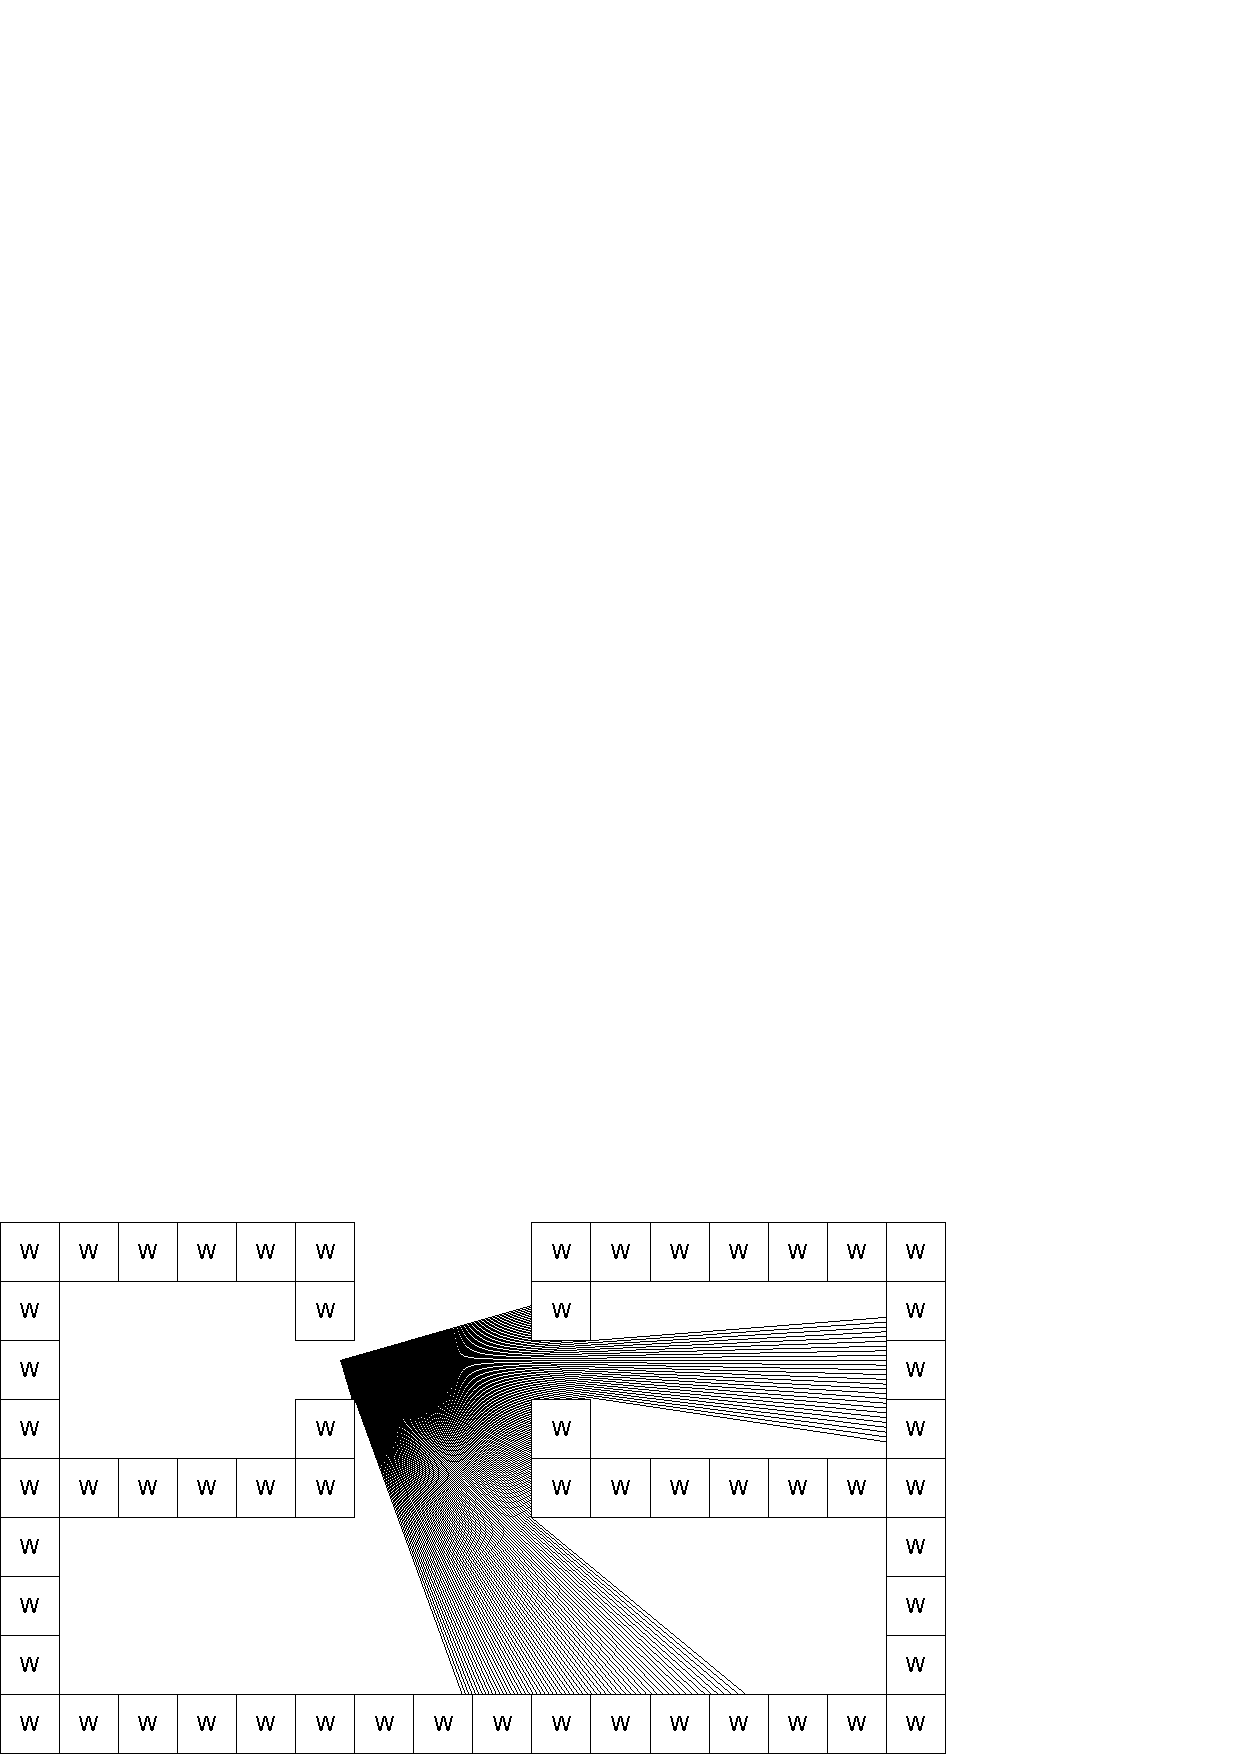
\includegraphics[width=\textwidth]{imgs/drawings/ray_caster_explained/out_room.pdf}
 \caption{Casting 320 rays (one for each column) for a screen of resolution 320x200} \label{fig:Raycasting2}
\end{figure}

\begin{figure}[H]
  \centering
 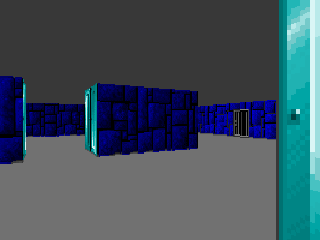
\includegraphics[width=\textwidth]{imgs/drawings/ray_caster_explained/out_door.png}
 \caption{Rendition of the 320 column of pixels (with texturing).} 
\end{figure} 















\subsection{Life of a Frame}
As we saw when we unrolled the loop, the action scene is made of frames in a loop, which in pseudo code looks as follows:\\
\par
\begin{minipage}{\textwidth}
 \lstinputlisting[language=C]{code/flawded_game_loop.c}
 \end{minipage}
\par
This is a pretty standard design for an engine from the early 90s. However, it has a major flaw: each slice of the game has a different duration depending on how long it takes to render and update. This variability makes the game nondeterministic between two machines, or even between two runs on the same machine. In the next drawing, all three timeslices representing three frames have different durations.\\
\begin{figure}[H]
\centering
 \includegraphics[width=\textwidth]{imgs/drawings/timer/wrong.pdf}
 
 \end{figure}
  At the beginning of each frame, the engine retrieves user inputs and combines them with the duration of the previous frame to update the world. Even if inputs are recorded for each frame, the same game could not be replayed as upon replaying a recorded game the engine would invariably reach a point where no inputs are available because a frame took more or less time to render. A simple disk access taking longer could have altered the duration of a frame, resulting in a different world outcome.\\
 \begin{figure}[H]
\centering
 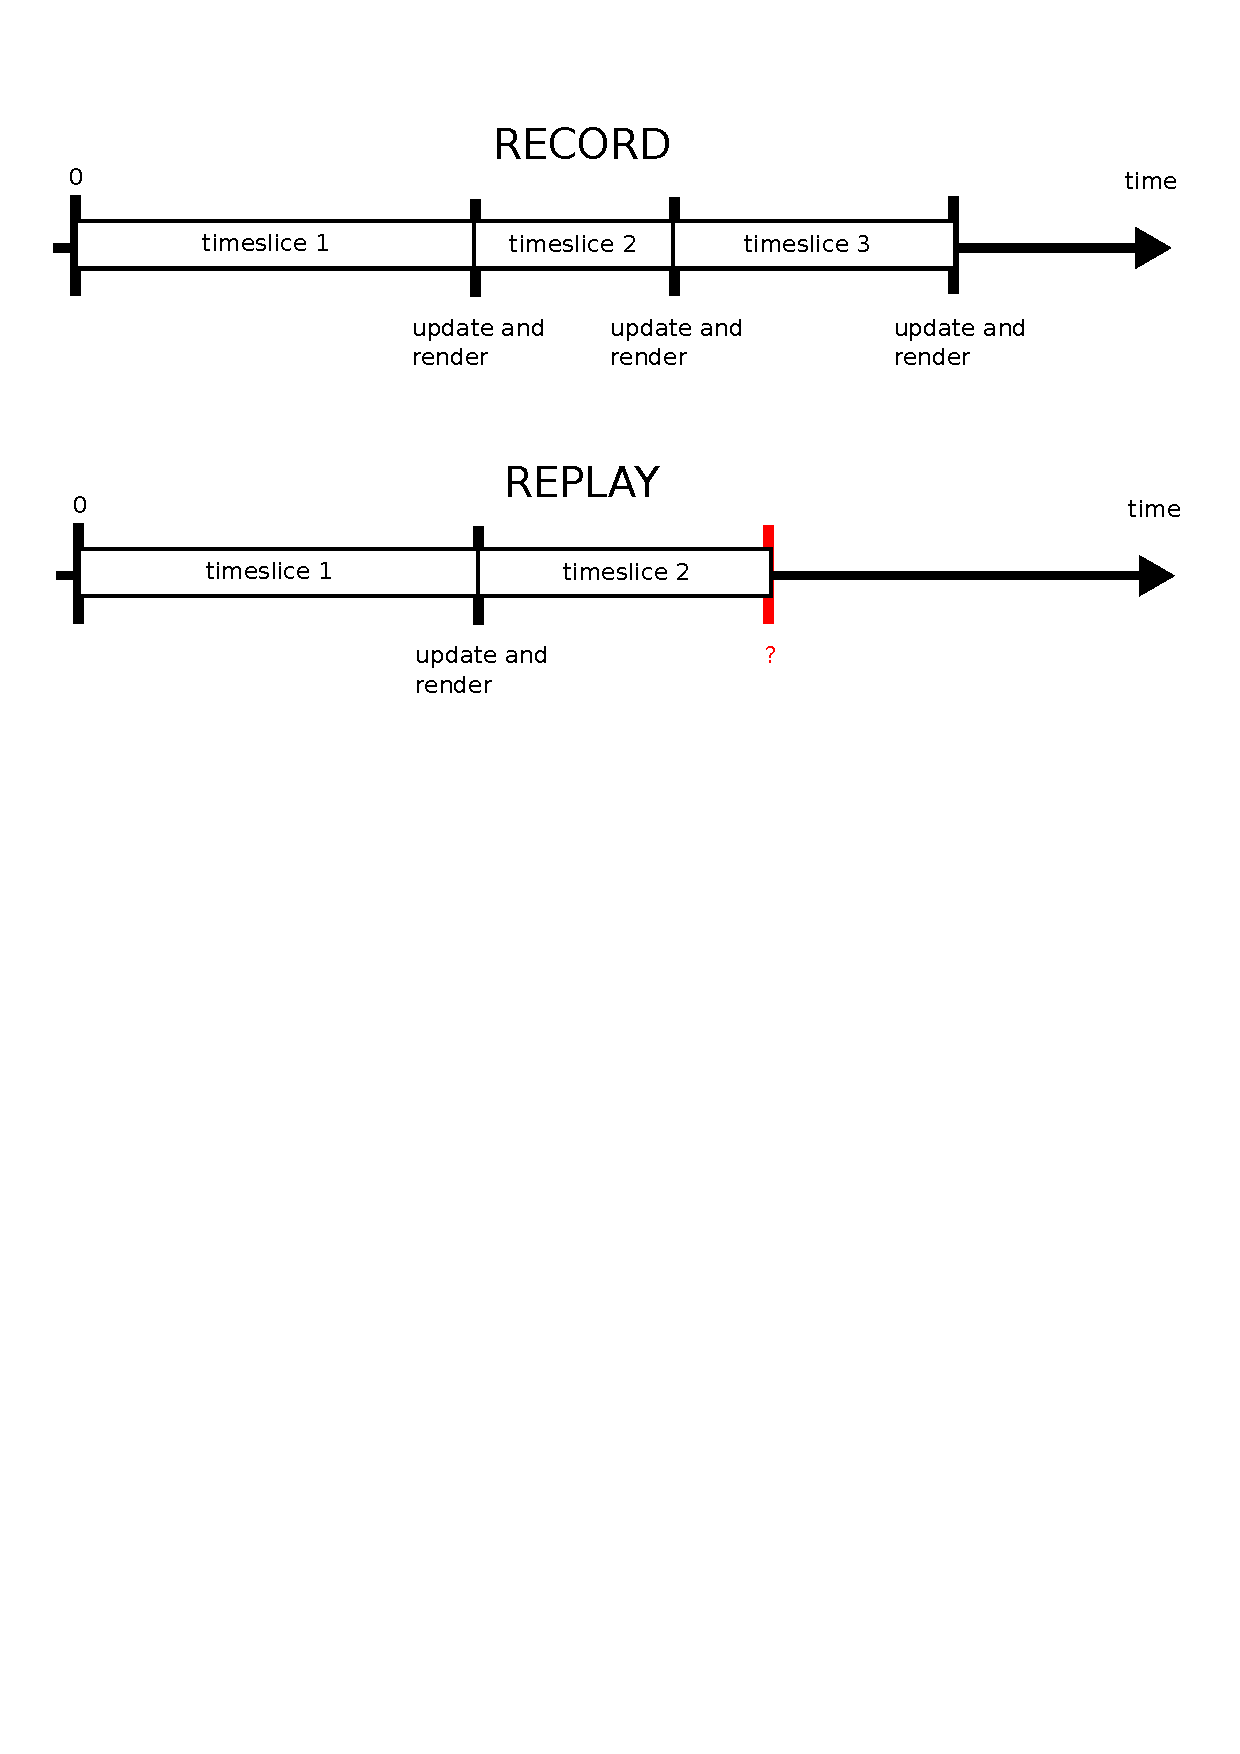
\includegraphics[width=\textwidth]{imgs/drawings/timer/replay.pdf}
 \caption{The second frame took longer to be rendered during the replay. No inputs are available for the player. Replay is now out of sync.}
 \end{figure}
\par
To solve this problem during the demo playback (shipped with the game), the engine disregards the heartbeats and simulates events at fixed interval (\cw{DEMOTICK} = 4)\footnote{70/4 = 17.5, the machine used to record the demo ran at 17 fps. Probably a high end 386.}. This hack resulted in a slower playback on 286 CPUs and faster playback on 486 CPUs (because it was recorded on a 386DX).\\
\par
In 1993, the Doom engine would solve this issue by simulating the world at fixed intervals\footnote{Doom run at a fixed rate of 35 fps.}.\\
\par
\begin{minipage}{\textwidth}
 \lstinputlisting[language=C]{code/fixed_game_loop.c}
 \end{minipage}
\par
This design decouples the renderer from the world updates. Timeslices are always the same duration. User inputs can be recorded and replayed without getting out of sync.
\par
 \begin{figure}[H]
\centering
 \includegraphics[width=\textwidth]{imgs/drawings/timer/fixed.pdf}
 \end{figure}

\begin{fancyquotes}
 Fixed versus variable game tic rates is still a debate today!  Doom using a locked tic rate made demos easy, but it also limited it to 35 fps, which later Pentium computers could get restricted by.\\
\par
\textbf{John Carmack - Programmer}
 \end{fancyquotes}










\subsection{Life of a 3D Frame}
Five stages are involved in drawing a 3D scene:\\
\begin{enumerate}
 \item Clear the framebuffer by drawing the floor and the ceiling (both solid colors).
 \item For each column of pixels on screen, cast a ray from the player to the nearest wall. Draw a textured column of pixels with height inversely proportional to the distance.
 \item Draw the sprites (enemies, lamps, barrels).
 \item Draw the weapon\footnote{A modern 3D engine would render the weapon first and leverage the depth buffer to save fillrate. In that era, however, memory access was so slow it was faster to accept a bit of overdraw.}.	
 \item Flip buffers: instruct CRT Controller to use the framebuffer just composed on next vsync.
\end{enumerate}
In the next six screenshots, the engine has been modified to slow down in order to see the content of the framebuffer at the end of each stage.\\
\begin{figure}[H]
\centering
 \fullimage{wolf3d_1_background.png}
 \caption{Stage 1: Clear screen}
 \end{figure}




\begin{figure}[H]
 \centering
  \fullimage{wolf3d_4_partial_wall_32rays.png}
  \caption{Stage 2: Drawing Walls: 15 rays} 
\end{figure}
\begin{minipage}{.4\textwidth}
Notice how the length of each ray corresponds to the height of a column in order to achieve perspective.\\
\par
The longer the distance the ray traveled, the shorter the column is drawn on screen.
 \end{minipage}
\begin{minipage}{.6\textwidth}
\begin{figure}[H]
  \centering
 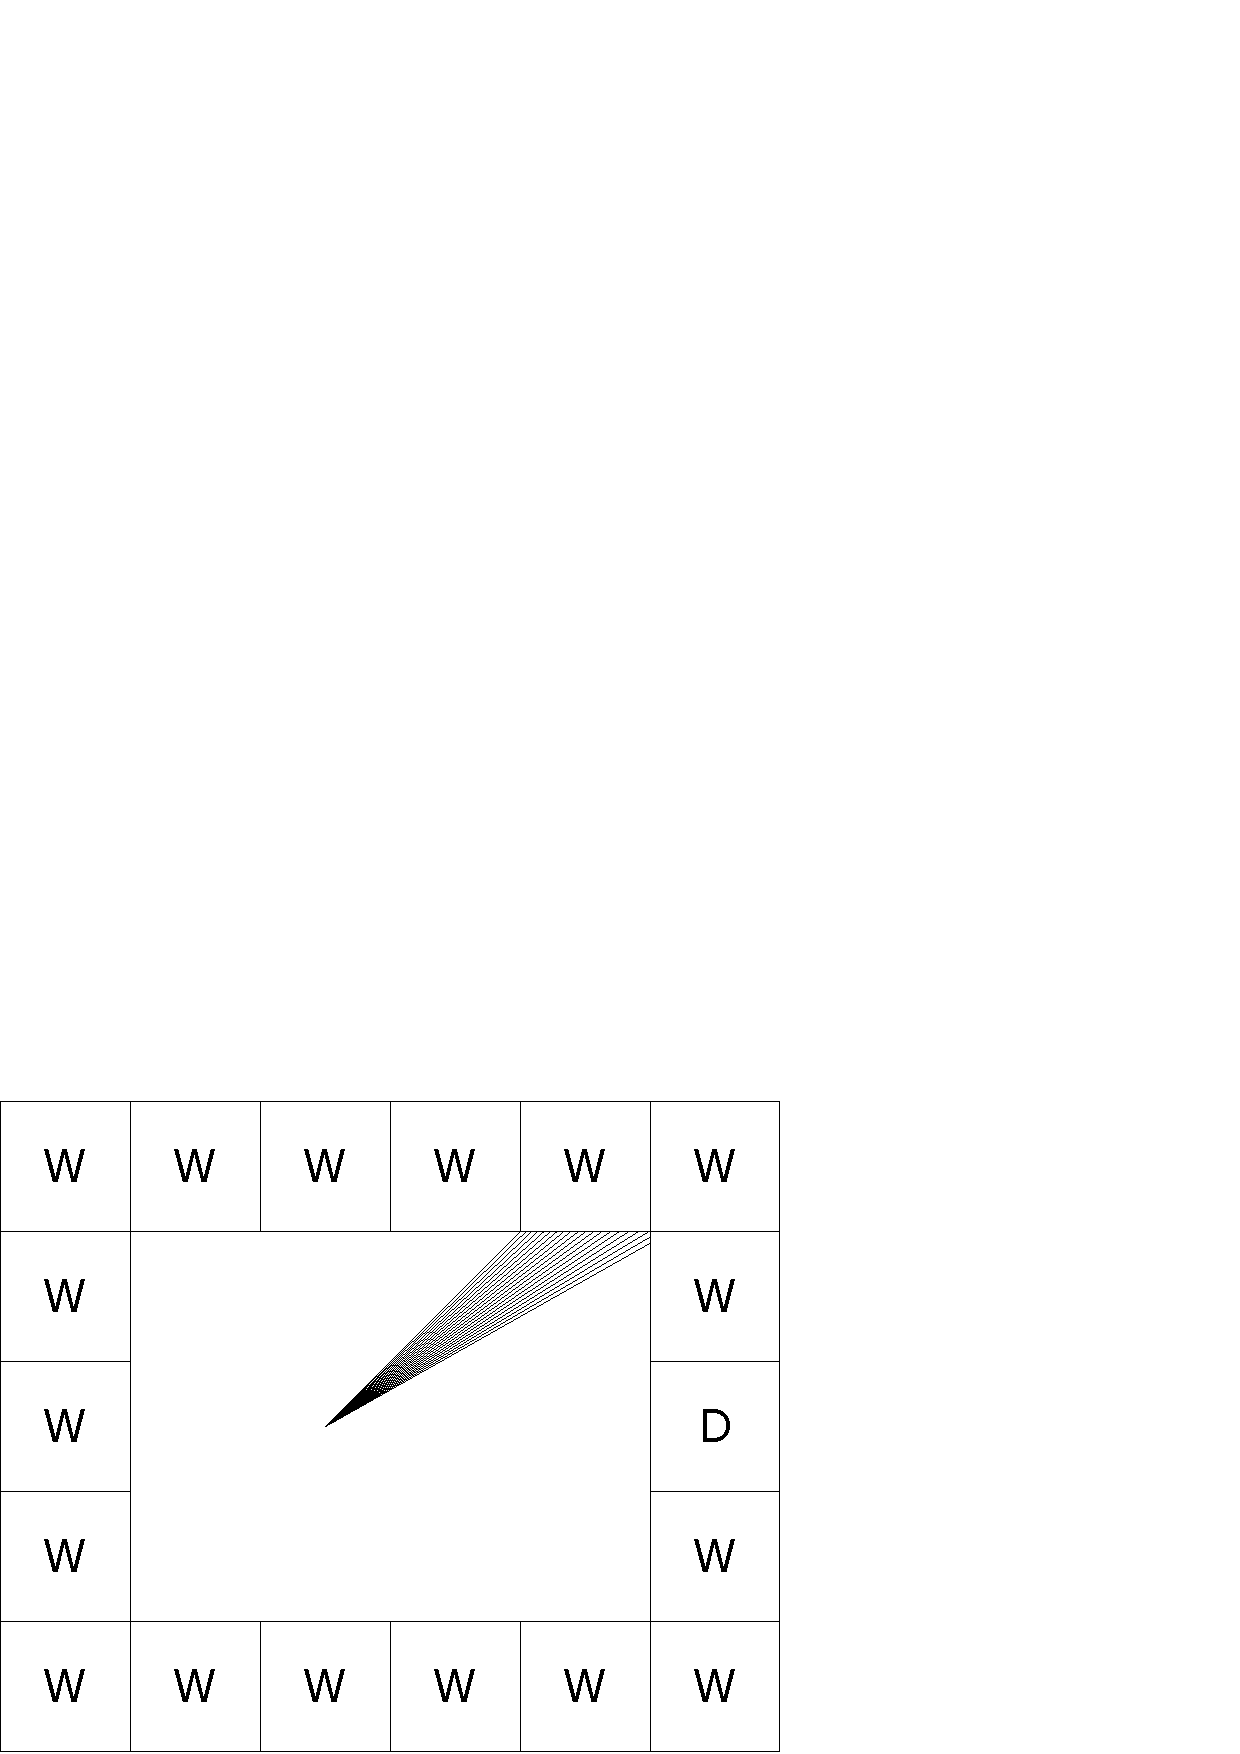
\includegraphics[width=.9\textwidth]{imgs/drawings/ray_caster_explained/beginning10.pdf}
   
\end{figure}
\end{minipage}




 
\begin{figure}[H]
 \centering
  \fullimage{wolf3d_5_partialwalls_160rays.png}
 \caption{Stage 2: Drawing Walls: 160 rays}  
\end{figure}
 \begin{minipage}{.4\textwidth}
 Doors are not sprites, they are part of the solid world. Notice how on the map a door is block aligned with the wall yet is rendered farther for perspective.\\
 \par
 The raycaster recognizes door tiles and injects a delta to the distance a ray traveled. If the door is partially open, the raycaster is also able to detect if the ray should stop or be allowed to traverse the tile.
 \end{minipage}
\begin{minipage}{.6\textwidth}
\begin{figure}[H]
  \centering
 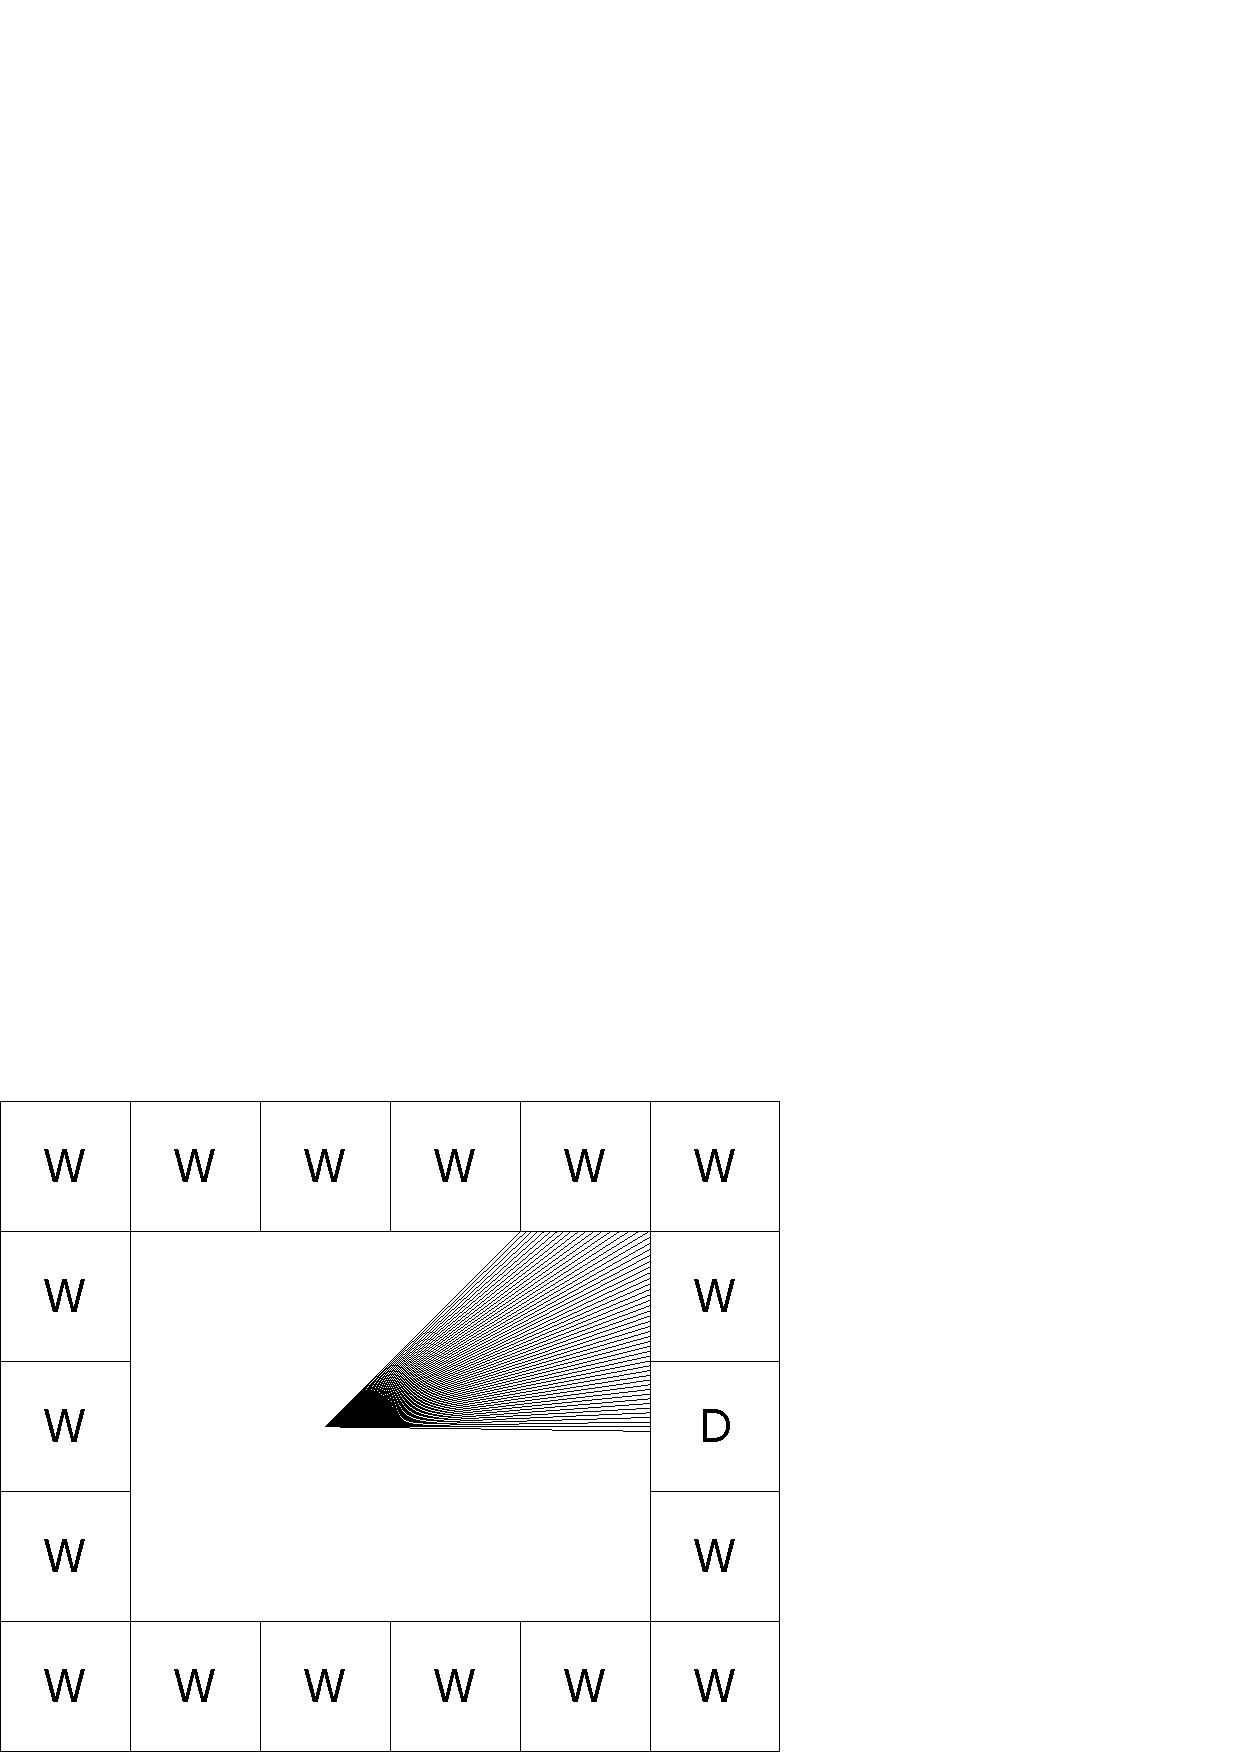
\includegraphics[width=.9\textwidth]{imgs/drawings/ray_caster_explained/beginning50.pdf}
   
\end{figure}
\end{minipage}



 
 \begin{figure}[H]
\centering
 \fullimage{wolf3d_2_walls.png}
 \caption{Stage 2: Drawing Walls has completed.} 
 \end{figure}
\begin{minipage}{\textwidth}
\begin{figure}[H]
  \centering
 
\includegraphics[width=.5\textwidth]{imgs/drawings/ray_caster_explained/beginning.pdf}
   
\end{figure}
\end{minipage}




 
 
 \begin{figure}[H]
\centering
 \fullimage{wolf3d_6_scaled}
 \caption{Stage 3: Drawing Things (a.k.a: Scaled, a.k.a: Sprites)} 
 \end{figure}
 After the raycaster is done, "things" are rendered. During this step, clipping is performed against the wall and doors.




 \begin{figure}[H]
\centering
 \fullimage{wolf3d_7_fullframe.png}
 \caption{Stage 4: Drawing Weapon} 
 \end{figure}
 













\subsection{3D Setup}
Before starting to draw frames, the 3D renderer sets up the VRAM with static elements forming the HUD\footnote{Heads-Up Display.}: the green background, the blue status bar, and all labels ("LEVEL", "SCORE", "LIVES", "HEALTH", and "AMMO").\\
\par
 \begin{fancyquotes}
   Wolfenstein was the last Id game that still had the concept of score and lives.  We were still in a quarter-eating-arcade-game design mode. With Doom, you finally got to just keep playing as long as you wanted, which was a bit radical at the time!
 \bigskip \\
\textbf{John Carmack - Programmer}
 \end{fancyquotes}
\begin{figure}[H]
  \centering
 \fullimage{hud_empty.png}
\end{figure}
This HUD is drawn only once at the beginning of the 3D phase. It has to be drawn in all three pages. For each new frame, the engine draws the 3D view in the reserved white canvas in the center. Small portions at the bottom of the HUD are updated: Level, Score, Lives, Status, Health, Ammo, and Current Weapon receive special treatment via another VGA trick in order to speed up rendition.\\
\par

The hardware chapter described Mode \cw{12h}, which despite being unfit for games still has an interesting characteristic. Mode \cw{12h} is a 16 color mode where each pixel color index is contained in a nibble. The four bits are spread across the four VGA banks. Since all write operations are one byte wide, it is not hard to imagine the difficulty in plotting a single pixel without changing the others stored in the same byte. One would have to do four read, four xor, and four writes. Since the designers of the VGA were not complete sadists, they added some circuitry to simplify this operation. For each bank, they created a latch placed in front of a configurable ALU.\\
\par
 \begin{figure}[H]
\centering
 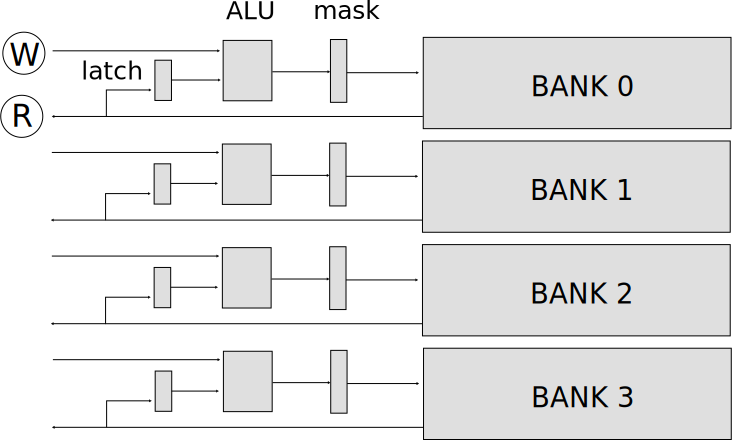
\includegraphics[width=\textwidth]{imgs/drawings/latches.pdf}
 \caption{Latches memorize read operation from each bank. The memorized value can be used for later writes.}
 \end{figure}
With this architecture, each time the VRAM is read \circled{R}, the latch from the corresponding bank is loaded with the read value. Each time a value is written to the VRAM \circled{W}, it can be composited by the ALU using the latched value and the written value. This design allowed mode \cw{12h} programmers to plot a pixel easily with one read, one ALU setup, and one write instead of four reads, 4 xors, and 4 writes.\\
\par
Mode Y does not need latches to operate since values are stored in bytes, and banks can be updated individually thanks to the mask. However, tinkerers\footnote{Michael Abrash Graphic Programming Black Book: Chapter 48 -- Mode X Marks the Latch.} found that these latches are still active in  Mode-Y. By getting a little creative, the circuitry can be re-purposed. The ALU in front of each bank can be setup to use only the latch for writing. With such a setup, upon doing one read, four latches are populated at once and four bytes in the bank are written with only one write to the RAM. This system allows transfer from VRAM to VRAM 4 bytes at a time.\\
\par
To take full advantage of this optimization, the 3D renderer uploads images to the VRAM above the third page. In total, the 43 sprites used to update the HUD are loaded in the asset page when the engine starts up.\\




\begin{minipage}{.3\textwidth}
     \fullimage{latched/109.png}
  \end{minipage}
\begin{minipage}{.3\textwidth}
     \fullimage{latched/110.png}
  \end{minipage}
\begin{minipage}{.3\textwidth}
     \fullimage{latched/111.png}
  \end{minipage}
\par



\begin{minipage}{.3\textwidth}
     \fullimage{latched/112.png}
  \end{minipage}
\begin{minipage}{.3\textwidth}
     \fullimage{latched/113.png}
  \end{minipage}
\begin{minipage}{.3\textwidth}
     \fullimage{latched/114.png}
  \end{minipage}
\par



  \begin{minipage}{.3\textwidth}
     \fullimage{latched/115.png}
  \end{minipage}
\begin{minipage}{.3\textwidth}
     \fullimage{latched/116.png}
  \end{minipage}
\begin{minipage}{.3\textwidth}
     \fullimage{latched/117.png}
  \end{minipage}
\par





  \begin{minipage}{.3\textwidth}
     \fullimage{latched/118.png}
  \end{minipage}
\begin{minipage}{.3\textwidth}
     \fullimage{latched/119.png}
  \end{minipage}
\begin{minipage}{.3\textwidth}
     \fullimage{latched/120.png}
  \end{minipage}
\par



  \begin{minipage}{.3\textwidth}
     \fullimage{latched/121.png}
  \end{minipage}
\begin{minipage}{.3\textwidth}
     \fullimage{latched/122.png}
  \end{minipage}
\begin{minipage}{.3\textwidth}
     \fullimage{latched/123.png}
  \end{minipage}
\par

    \begin{minipage}{.3\textwidth}
     \fullimage{latched/124.png}
  \end{minipage}
\begin{minipage}{.3\textwidth}
     \fullimage{latched/125.png}
  \end{minipage}
\begin{minipage}{.3\textwidth}
     \fullimage{latched/126.png}
  \end{minipage}
\par


\begin{minipage}{.328\textwidth}
     \fullimage{latched/127.png}
  \end{minipage}
\begin{minipage}{.328\textwidth}
     \fullimage{latched/128.png}
  \end{minipage}
\begin{minipage}{.328\textwidth}
     \fullimage{latched/129.png}
  \end{minipage}
\par

\begin{minipage}{.328\textwidth}
     \fullimage{latched/130.png}
  \end{minipage}
\begin{minipage}{.328\textwidth}
     \fullimage{latched/131.png}
  \end{minipage}
\begin{minipage}{.328\textwidth}
     \fullimage{latched/132.png}
  \end{minipage}
\par

\begin{minipage}{.245\textwidth}
     \fullimage{latched/91.png}
  \end{minipage}
\begin{minipage}{.245\textwidth}
     \fullimage{latched/92.png}
  \end{minipage}
\begin{minipage}{.245\textwidth}
     \fullimage{latched/93.png}
  \end{minipage}
\begin{minipage}{.245\textwidth}
     \fullimage{latched/94.png}
  \end{minipage}
\par


\begin{minipage}{.095\textwidth}
     \fullimage{latched/99.png}
  \end{minipage}
\begin{minipage}{.095\textwidth}
     \fullimage{latched/100.png}
  \end{minipage}
\begin{minipage}{.095\textwidth}
     \fullimage{latched/101.png}
  \end{minipage}
\begin{minipage}{.095\textwidth}
     \fullimage{latched/102.png}
  \end{minipage}
\begin{minipage}{.095\textwidth}
     \fullimage{latched/103.png}
  \end{minipage}
\begin{minipage}{.095\textwidth}
     \fullimage{latched/104.png}
  \end{minipage}
\begin{minipage}{.095\textwidth}
     \fullimage{latched/105.png}
  \end{minipage}
\begin{minipage}{.095\textwidth}
     \fullimage{latched/106.png}
  \end{minipage}
\begin{minipage}{.095\textwidth}
     \fullimage{latched/107.png}
  \end{minipage}
\begin{minipage}{.095\textwidth}
     \fullimage{latched/108.png}
  \end{minipage}
\par


\begin{minipage}{.1\textwidth}
     \fullimage{latched/95.png}
  \end{minipage}
\begin{minipage}{.1\textwidth}
     \fullimage{latched/96.png}
  \end{minipage}
\begin{minipage}{.1\textwidth}
     \fullimage{latched/97.png}
  \end{minipage}
\begin{minipage}{.1\textwidth}
     \fullimage{latched/98.png}
  \end{minipage}
  \begin{minipage}{.3\textwidth}
     \fullimage{latched/133.png}
  \end{minipage}
\begin{minipage}{.3\textwidth}
     \fullimage{latched/134.png}
  \end{minipage}\

\bu{Trick :} Images are stored woven. All bytes for bank 0, then all bytes for bank 1, and so on. This clever way to store data allows a bank to be loaded very fast with one \cw{memcpy} per bank (four \cw{memcpy} per image).\\
\par
All these assets account for 48*24*4 (weapons sprites) + 14*8*16 (numeral and key sprites) + 24*24*32 (face sprites) + 224 * 48 (paused + psyched) = 34,816 bytes. There are therefore 35,324 unused bytes in the fourth VGA page.\\
\par
For this trick to work, image sources and destinations have to be aligned on four bytes horizontally in screen space. If you take a look at the location of each element on screen you can see that elements are aligned on four pixels horizontally but there is no such constraint vertically.
\begin{figure}[H]
  \centering
 \includegraphics[width=\textwidth]{imgs/drawings/hud.pdf}
\end{figure}

While it is faster to copy four pixels in one read and one write, this trick does not provide a full 400\% speed increase as all writes have to be done in all three screen pages. This is obvious when looking at the routine for updating the status (hero's face).\\
\par
\begin{minipage}{\textwidth}
\lstinputlisting[language=C]{code/StatusDrawPic.c}
\end{minipage}
\par
This optimization still results in a 30\% overall speed increase.\\
\par











\subsection{Clearing the Screen}
At the beginning of a frame, the engine switches to the next page and clears the 3D area with ceiling and floor colors. To create this effect, it uses the same trick seen in the 2D renderer and sets the VGA bank mask to 15 to write to all banks simultaneously. Since values are written 16 bits at a time, it can write 8 pixels at a time.\\ 
\par
\scaledimage{1}{clear_screen_pixels}


\begin{minipage}{\textwidth}
 \lstinputlisting[language=C,morekeywords=asm]{code/VGAClearScreen.c}
 \end{minipage}
\par
Clearing the 3D canvas made of 304*152 = 46,208 pixels requires only 27 instructions thanks to \cw{REP STOSW}.\\
\par
Colors for the floor and the ceiling do not come from map data files. The ground is always the same color (\cw{0x19}) and ceiling colors are hardcoded in the engine on a per level basis.\\
\par
\begin{minipage}{\textwidth}
 \lstinputlisting[language=C,morekeywords=byte]{code/vgaCeiling.c}
 \end{minipage}
\par


Following are ceiling colors \cw{0x1D}, \cw{0xBF}, \cw{0x4E} and \cw{0x8D}.\\ 
\par
\scaledimage{.24}{palette_1d.png}
\scaledimage{.24}{palette_bf.png}
\scaledimage{.24}{palette_8d.png}
\scaledimage{.24}{palette_4e.png}












\subsection{Solving the CPU Problem}

In the Chapter \ref{chapter_hardware} \nameref{chapter_hardware} p\pageref{chapter_hardware} describing CPU capabilities, the reader was left with a problem: the machine cannot perform floating point operations quickly enough. This is a pretty big issue for a 3D engine given all the trigonometry involved. It turns out the solution is to trick the ALU via a technique called "fixed point arithmetic".







\subsubsection{Fixed Point}
The normal layout of an \cw{int} is as follows.
\begin{figure}[H]
\centering
 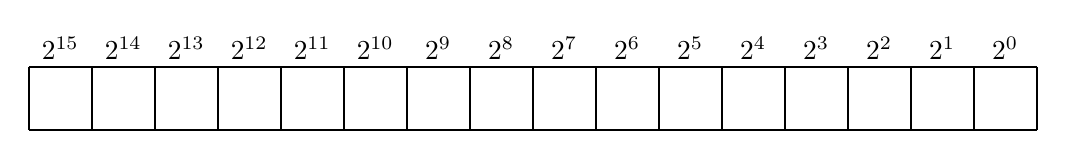
\begin{tikzpicture}[scale=0.8, every node/.style={scale=0.99}]
\draw[thick] (0,0) -- (16,0);
\draw[thick] (0,1) -- (16,1);
\foreach \i in {0,...,16}
{
     \draw[thick] (\i,1) -- (\i,0);
}

\foreach \i in {0,...,15}
{
     \node[] at (15-\i+0.5,1.3){$2^{\i}$}  ;
       
       
     
}
\end{tikzpicture}

 \caption{Integer layout.} \label{fig:int_layout}
 \end{figure}
The value of the sequence of bits \emph{0010010010010010}:
\begin{figure}[H]
\centering
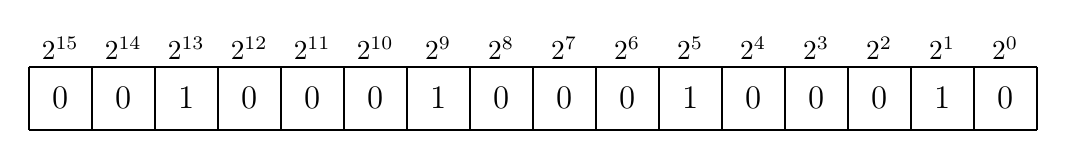
\begin{tikzpicture}[scale=0.8, every node/.style={scale=0.99}]
\draw[thick] (0,0) -- (16,0);
\draw[thick] (0,1) -- (16,1);
\foreach \i in {0,...,16}
{
     \draw[thick] (\i,1) -- (\i,0);
}

\foreach \i in {0,...,15}
{
     \node[] at (15-\i+0.5,1.3){$2^{\i}$}  ;
}

\tikzstyle{fontbf} = [font=\large]
\node[fontbf] at (0.5,0.5){0} ;
\node[fontbf] at (1.5,0.5){0};  
\node[fontbf] at (2.5,0.5){1} ; 
\node[fontbf] at (3.5,0.5){0} ;

\node[fontbf] at (4.5,0.5){0} ;
\node[fontbf] at (5.5,0.5){0};  
\node[fontbf] at (6.5,0.5){1} ; 
\node[fontbf] at (7.5,0.5){0} ;

\node[fontbf] at (8.5,0.5){0} ;
\node[fontbf] at (9.5,0.5){0};  
\node[fontbf] at (10.5,0.5){1} ; 
\node[fontbf] at (11.5,0.5){0} ;

\node[fontbf] at (12.5,0.5){0} ;
\node[fontbf] at (13.5,0.5){0};  
\node[fontbf] at (14.5,0.5){1} ; 
\node[fontbf] at (15.5,0.5){0} ;


\end{tikzpicture}

 \end{figure}

Represents $ 2^{13} + 2^9 + 2^5 + 2^1 =  8738 $.\\
 \par

Fixed Point allows for keeping track of fractions while still using the integer operations of the CPU. The machine manipulates what are supposed to be integer numbers, but the programmer sees them as a value containing an integer part and a fractional part:\\
\par
\begin{figure}[H]
 \centering
  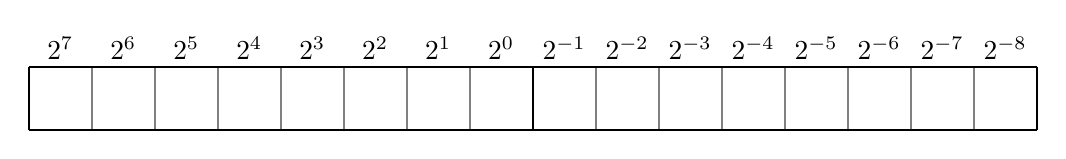
\begin{tikzpicture}[scale=0.8, every node/.style={scale=0.99}]


\colorlet{LighterMark}{black!50}

\foreach \i in {1,...,15}
{
     \draw[thick,LighterMark] (\i,1) -- (\i,0);
}

     \draw[thick,black] (0,1) -- (0,0);
      \draw[thick,black] (8,1) -- (8,0);
      \draw[thick,black] (16,1) -- (16,0);
      
\draw[thick,black] (0,0) -- (16,0);
\draw[thick,black] (0,1) -- (16,1);
 

%\foreach \i[evaluate={\pow=int(7-\i)}] in {0,...,7}
\foreach \i[evaluate={\pow=int(7-\i)}] in {0,...,7}
{
   \node[] at (\i+0.5,1.3){$2^{\pow}$  }  ;
      
         
     
}

%\foreach \i[evaluate={\pow=int((\i-7)*2)}]  in {8,...,15}
\foreach \i[evaluate={\pow=int(\i-7)}]  in {8,...,15}
{
     \node[] at (\i+0.5,1.3){$2^{-\pow}$}  ;
}




\end{tikzpicture}

 \caption{Fixed point layout 8:8 (8 bits for the integer part and 8 bits for the fractional part).} \label{fig:mips}
\end{figure}

The same sequence of bits \emph{0010010010010010} with different powers of two...
\begin{figure}[H]
 \centering
   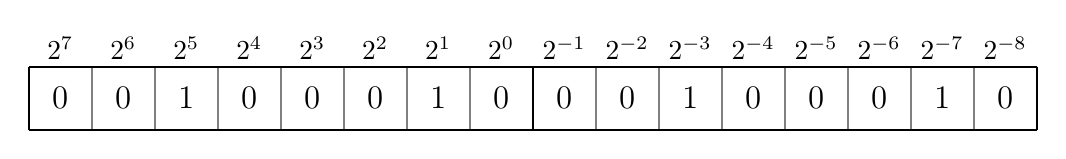
\begin{tikzpicture}[scale=0.8, every node/.style={scale=0.99}]


\colorlet{LighterMark}{black!50}

\foreach \i in {1,...,15}
{
     \draw[thick,LighterMark] (\i,1) -- (\i,0);
}

     \draw[thick,black] (0,1) -- (0,0);
      \draw[thick,black] (8,1) -- (8,0);
      \draw[thick,black] (16,1) -- (16,0);
      
\draw[thick,black] (0,0) -- (16,0);
\draw[thick,black] (0,1) -- (16,1);
 

%\foreach \i[evaluate={\pow=int(7-\i)}] in {0,...,7}
\foreach \i[evaluate={\pow=int(7-\i)}] in {0,...,7}
{
   \node[] at (\i+0.5,1.3){$2^{\pow}$  }  ;
      
         
     
}

%\foreach \i[evaluate={\pow=int((\i-7)*2)}]  in {8,...,15}
\foreach \i[evaluate={\pow=int(\i-7)}]  in {8,...,15}
{
     \node[] at (\i+0.5,1.3){$2^{-\pow}$}  ;
}

\tikzstyle{fontbf} = [font=\large]
\node[fontbf] at (0.5,0.5){0} ;
\node[fontbf] at (1.5,0.5){0};  
\node[fontbf] at (2.5,0.5){1} ; 
\node[fontbf] at (3.5,0.5){0} ;

\node[fontbf] at (4.5,0.5){0} ;
\node[fontbf] at (5.5,0.5){0};  
\node[fontbf] at (6.5,0.5){1} ; 
\node[fontbf] at (7.5,0.5){0} ;

\node[fontbf] at (8.5,0.5){0} ;
\node[fontbf] at (9.5,0.5){0};  
\node[fontbf] at (10.5,0.5){1} ; 
\node[fontbf] at (11.5,0.5){0} ;

\node[fontbf] at (12.5,0.5){0} ;
\node[fontbf] at (13.5,0.5){0};  
\node[fontbf] at (14.5,0.5){1} ; 
\node[fontbf] at (15.5,0.5){0} ;


\end{tikzpicture}

\end{figure} 

Now represents:\\

$ 2^5 + 2^1 = 34 $ for the integer part.\\
$ 2^{-3}+2^{-7} = 0.1328125 $ for the fractional part.\\
$ = 34.1328125$\\

\bigskip

The beauty of fixed point is that addition and subtraction work exactly like integers from the CPU instruction side.\\




\par
\begin{figure}[H]
 \centering
   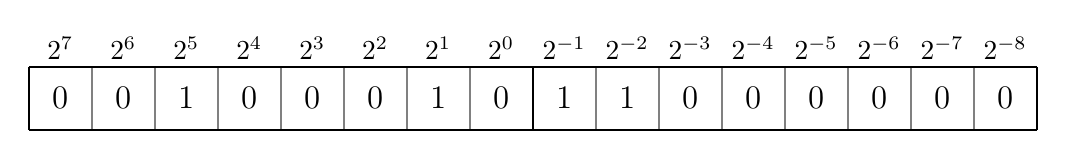
\begin{tikzpicture}[scale=0.8, every node/.style={scale=0.99}]


\colorlet{LighterMark}{black!50}

\foreach \i in {1,...,15}
{
     \draw[thick,LighterMark] (\i,1) -- (\i,0);
}

     \draw[thick,black] (0,1) -- (0,0);
      \draw[thick,black] (8,1) -- (8,0);
      \draw[thick,black] (16,1) -- (16,0);
      
\draw[thick,black] (0,0) -- (16,0);
\draw[thick,black] (0,1) -- (16,1);
 

%\foreach \i[evaluate={\pow=int(7-\i)}] in {0,...,7}
\foreach \i[evaluate={\pow=int(7-\i)}] in {0,...,7}
{
   \node[] at (\i+0.5,1.3){$2^{\pow}$  }  ;
      
         
     
}

%\foreach \i[evaluate={\pow=int((\i-7)*2)}]  in {8,...,15}
\foreach \i[evaluate={\pow=int(\i-7)}]  in {8,...,15}
{
     \node[] at (\i+0.5,1.3){$2^{-\pow}$}  ;
}

\tikzstyle{fontbf} = [font=\large]
\node[fontbf] at (0.5,0.5){0} ;
\node[fontbf] at (1.5,0.5){0};  
\node[fontbf] at (2.5,0.5){1} ; 
\node[fontbf] at (3.5,0.5){0} ;

\node[fontbf] at (4.5,0.5){0} ;
\node[fontbf] at (5.5,0.5){0};  
\node[fontbf] at (6.5,0.5){1} ; 
\node[fontbf] at (7.5,0.5){0} ;

\node[fontbf] at (8.5,0.5){1} ;
\node[fontbf] at (9.5,0.5){1};  
\node[fontbf] at (10.5,0.5){0} ; 
\node[fontbf] at (11.5,0.5){0} ;

\node[fontbf] at (12.5,0.5){0} ;
\node[fontbf] at (13.5,0.5){0};  
\node[fontbf] at (14.5,0.5){0} ; 
\node[fontbf] at (15.5,0.5){0} ;


\end{tikzpicture}


   \caption{34.75} 
\end{figure} 

\begin{figure}[H]
 \centering
   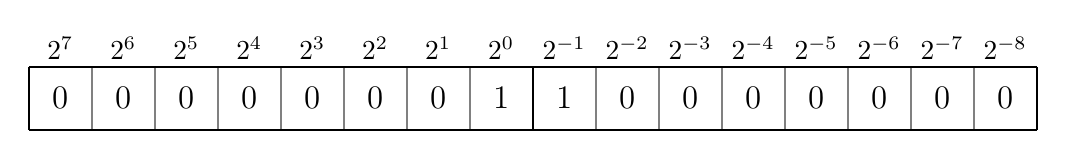
\begin{tikzpicture}[scale=0.8, every node/.style={scale=0.99}]


\colorlet{LighterMark}{black!50}

\foreach \i in {1,...,15}
{
     \draw[thick,LighterMark] (\i,1) -- (\i,0);
}

     \draw[thick,black] (0,1) -- (0,0);
      \draw[thick,black] (8,1) -- (8,0);
      \draw[thick,black] (16,1) -- (16,0);
      
\draw[thick,black] (0,0) -- (16,0);
\draw[thick,black] (0,1) -- (16,1);
 

%\foreach \i[evaluate={\pow=int(7-\i)}] in {0,...,7}
\foreach \i[evaluate={\pow=int(7-\i)}] in {0,...,7}
{
   \node[] at (\i+0.5,1.3){$2^{\pow}$  }  ;
      
         
     
}

%\foreach \i[evaluate={\pow=int((\i-7)*2)}]  in {8,...,15}
\foreach \i[evaluate={\pow=int(\i-7)}]  in {8,...,15}
{
     \node[] at (\i+0.5,1.3){$2^{-\pow}$}  ;
}

\tikzstyle{fontbf} = [font=\large]
\node[fontbf] at (0.5,0.5){0} ;
\node[fontbf] at (1.5,0.5){0};  
\node[fontbf] at (2.5,0.5){0} ; 
\node[fontbf] at (3.5,0.5){0} ;

\node[fontbf] at (4.5,0.5){0} ;
\node[fontbf] at (5.5,0.5){0};  
\node[fontbf] at (6.5,0.5){0} ; 
\node[fontbf] at (7.5,0.5){1} ;

\node[fontbf] at (8.5,0.5){1} ;
\node[fontbf] at (9.5,0.5){0};  
\node[fontbf] at (10.5,0.5){0} ; 
\node[fontbf] at (11.5,0.5){0} ;

\node[fontbf] at (12.5,0.5){0} ;
\node[fontbf] at (13.5,0.5){0};  
\node[fontbf] at (14.5,0.5){0} ; 
\node[fontbf] at (15.5,0.5){0} ;


\end{tikzpicture}

  \caption{1.5} 
\end{figure} 

\begin{figure}[H]
 \centering
   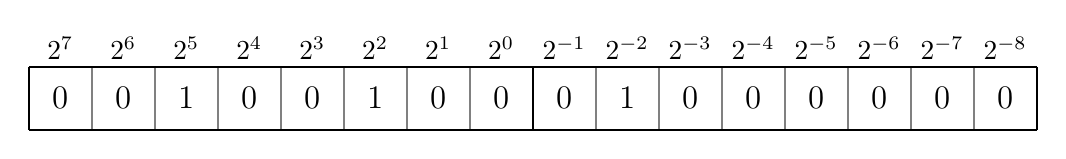
\begin{tikzpicture}[scale=0.8, every node/.style={scale=0.99}]


\colorlet{LighterMark}{black!50}

\foreach \i in {1,...,15}
{
     \draw[thick,LighterMark] (\i,1) -- (\i,0);
}

     \draw[thick,black] (0,1) -- (0,0);
      \draw[thick,black] (8,1) -- (8,0);
      \draw[thick,black] (16,1) -- (16,0);
      
\draw[thick,black] (0,0) -- (16,0);
\draw[thick,black] (0,1) -- (16,1);
 

%\foreach \i[evaluate={\pow=int(7-\i)}] in {0,...,7}
\foreach \i[evaluate={\pow=int(7-\i)}] in {0,...,7}
{
   \node[] at (\i+0.5,1.3){$2^{\pow}$  }  ;
      
         
     
}

%\foreach \i[evaluate={\pow=int((\i-7)*2)}]  in {8,...,15}
\foreach \i[evaluate={\pow=int(\i-7)}]  in {8,...,15}
{
     \node[] at (\i+0.5,1.3){$2^{-\pow}$}  ;
}

\tikzstyle{fontbf} = [font=\large]
\node[fontbf] at (0.5,0.5){0} ;
\node[fontbf] at (1.5,0.5){0};  
\node[fontbf] at (2.5,0.5){1} ; 
\node[fontbf] at (3.5,0.5){0} ;

\node[fontbf] at (4.5,0.5){0} ;
\node[fontbf] at (5.5,0.5){1};  
\node[fontbf] at (6.5,0.5){0} ; 
\node[fontbf] at (7.5,0.5){0} ;

\node[fontbf] at (8.5,0.5){0} ;
\node[fontbf] at (9.5,0.5){1};  
\node[fontbf] at (10.5,0.5){0} ; 
\node[fontbf] at (11.5,0.5){0} ;

\node[fontbf] at (12.5,0.5){0} ;
\node[fontbf] at (13.5,0.5){0};  
\node[fontbf] at (14.5,0.5){0} ; 
\node[fontbf] at (15.5,0.5){0} ;


\end{tikzpicture}

  {\caption{34.75 + 1.5= 36.25}}
\end{figure} 
\par
 Even right shift trick (divide by power of two) and left shift trick (multiply by power of two) work...\\
 
 \par
\begin{figure}[H]
 \centering
   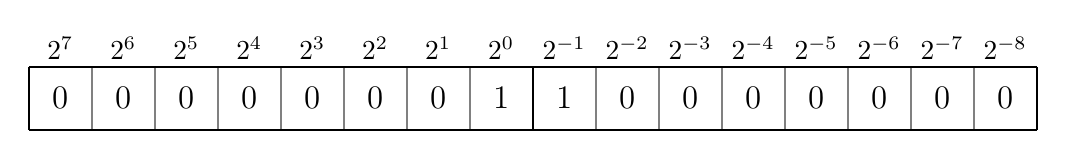
\begin{tikzpicture}[scale=0.8, every node/.style={scale=0.99}]


\colorlet{LighterMark}{black!50}

\foreach \i in {1,...,15}
{
     \draw[thick,LighterMark] (\i,1) -- (\i,0);
}

     \draw[thick,black] (0,1) -- (0,0);
      \draw[thick,black] (8,1) -- (8,0);
      \draw[thick,black] (16,1) -- (16,0);
      
\draw[thick,black] (0,0) -- (16,0);
\draw[thick,black] (0,1) -- (16,1);
 

%\foreach \i[evaluate={\pow=int(7-\i)}] in {0,...,7}
\foreach \i[evaluate={\pow=int(7-\i)}] in {0,...,7}
{
   \node[] at (\i+0.5,1.3){$2^{\pow}$  }  ;
      
         
     
}

%\foreach \i[evaluate={\pow=int((\i-7)*2)}]  in {8,...,15}
\foreach \i[evaluate={\pow=int(\i-7)}]  in {8,...,15}
{
     \node[] at (\i+0.5,1.3){$2^{-\pow}$}  ;
}

\tikzstyle{fontbf} = [font=\large]
\node[fontbf] at (0.5,0.5){0} ;
\node[fontbf] at (1.5,0.5){0};  
\node[fontbf] at (2.5,0.5){0} ; 
\node[fontbf] at (3.5,0.5){0} ;

\node[fontbf] at (4.5,0.5){0} ;
\node[fontbf] at (5.5,0.5){0};  
\node[fontbf] at (6.5,0.5){0} ; 
\node[fontbf] at (7.5,0.5){1} ;

\node[fontbf] at (8.5,0.5){1} ;
\node[fontbf] at (9.5,0.5){0};  
\node[fontbf] at (10.5,0.5){0} ; 
\node[fontbf] at (11.5,0.5){0} ;

\node[fontbf] at (12.5,0.5){0} ;
\node[fontbf] at (13.5,0.5){0};  
\node[fontbf] at (14.5,0.5){0} ; 
\node[fontbf] at (15.5,0.5){0} ;


\end{tikzpicture}

   \caption{1.5} 
\end{figure} 

\par
\begin{figure}[H]
 \centering
   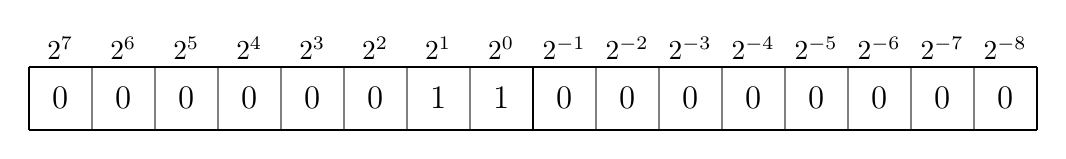
\begin{tikzpicture}[scale=0.8, every node/.style={scale=0.99}]


\colorlet{LighterMark}{black!50}

\foreach \i in {1,...,15}
{
     \draw[thick,LighterMark] (\i,1) -- (\i,0);
}

     \draw[thick,black] (0,1) -- (0,0);
      \draw[thick,black] (8,1) -- (8,0);
      \draw[thick,black] (16,1) -- (16,0);
      
\draw[thick,black] (0,0) -- (16,0);
\draw[thick,black] (0,1) -- (16,1);
 

%\foreach \i[evaluate={\pow=int(7-\i)}] in {0,...,7}
\foreach \i[evaluate={\pow=int(7-\i)}] in {0,...,7}
{
   \node[] at (\i+0.5,1.3){$2^{\pow}$  }  ;
      
         
     
}

%\foreach \i[evaluate={\pow=int((\i-7)*2)}]  in {8,...,15}
\foreach \i[evaluate={\pow=int(\i-7)}]  in {8,...,15}
{
     \node[] at (\i+0.5,1.3){$2^{-\pow}$}  ;
}

\tikzstyle{fontbf} = [font=\large]
\node[fontbf] at (0.5,0.5){0} ;
\node[fontbf] at (1.5,0.5){0};  
\node[fontbf] at (2.5,0.5){0} ; 
\node[fontbf] at (3.5,0.5){0} ;

\node[fontbf] at (4.5,0.5){0} ;
\node[fontbf] at (5.5,0.5){0};  
\node[fontbf] at (6.5,0.5){1} ; 
\node[fontbf] at (7.5,0.5){1} ;

\node[fontbf] at (8.5,0.5){0} ;
\node[fontbf] at (9.5,0.5){0};  
\node[fontbf] at (10.5,0.5){0} ; 
\node[fontbf] at (11.5,0.5){0} ;

\node[fontbf] at (12.5,0.5){0} ;
\node[fontbf] at (13.5,0.5){0};  
\node[fontbf] at (14.5,0.5){0} ; 
\node[fontbf] at (15.5,0.5){0} ;


\end{tikzpicture}

   \caption{1.5 << 1  = 3} 
\end{figure}

\par
\begin{figure}[H]
 \centering
   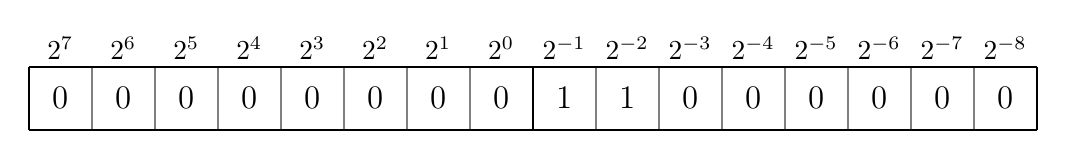
\begin{tikzpicture}[scale=0.8, every node/.style={scale=0.99}]


\colorlet{LighterMark}{black!50}

\foreach \i in {1,...,15}
{
     \draw[thick,LighterMark] (\i,1) -- (\i,0);
}

     \draw[thick,black] (0,1) -- (0,0);
      \draw[thick,black] (8,1) -- (8,0);
      \draw[thick,black] (16,1) -- (16,0);
      
\draw[thick,black] (0,0) -- (16,0);
\draw[thick,black] (0,1) -- (16,1);
 

%\foreach \i[evaluate={\pow=int(7-\i)}] in {0,...,7}
\foreach \i[evaluate={\pow=int(7-\i)}] in {0,...,7}
{
   \node[] at (\i+0.5,1.3){$2^{\pow}$  }  ;
      
         
     
}

%\foreach \i[evaluate={\pow=int((\i-7)*2)}]  in {8,...,15}
\foreach \i[evaluate={\pow=int(\i-7)}]  in {8,...,15}
{
     \node[] at (\i+0.5,1.3){$2^{-\pow}$}  ;
}

\tikzstyle{fontbf} = [font=\large]
\node[fontbf] at (0.5,0.5){0} ;
\node[fontbf] at (1.5,0.5){0};  
\node[fontbf] at (2.5,0.5){0} ; 
\node[fontbf] at (3.5,0.5){0} ;

\node[fontbf] at (4.5,0.5){0} ;
\node[fontbf] at (5.5,0.5){0};  
\node[fontbf] at (6.5,0.5){0} ; 
\node[fontbf] at (7.5,0.5){0} ;

\node[fontbf] at (8.5,0.5){1} ;
\node[fontbf] at (9.5,0.5){1};  
\node[fontbf] at (10.5,0.5){0} ; 
\node[fontbf] at (11.5,0.5){0} ;

\node[fontbf] at (12.5,0.5){0} ;
\node[fontbf] at (13.5,0.5){0};  
\node[fontbf] at (14.5,0.5){0} ; 
\node[fontbf] at (15.5,0.5){0} ;


\end{tikzpicture}

   \caption{1.5 >> 1 = 0.75} 
\end{figure}

The notation for fixed point is \cw{BITS\_FOR\_INTEGER\_PART:BITS\_FOR\_FRACTIONAL\_PART}. In the game, the player's position is \cw{16:16}. The grid location is one shift operation away \cw{player->x $\gg$ 16}.\\
\par
Performing multiplication and division are special cases. There are two ways to do this: either multiply two 32 bit values into 64 bits (and drop the upper and lower 16 bits) or drop the precision of both fixed point values and then multiply them into 32 bits. Both methods involve accepting a loss of data via overflow or underflow. Let's take the example of $98.7539 * 1.5$.


\par
\begin{figure}[H]
 \centering
   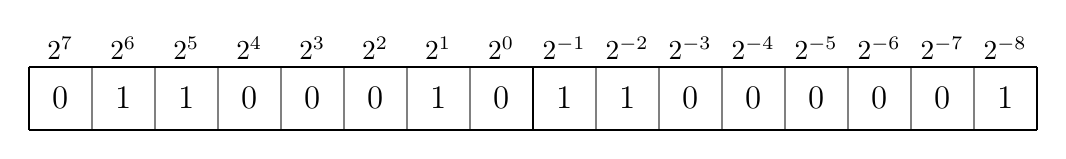
\begin{tikzpicture}[scale=0.8, every node/.style={scale=0.99}]


\colorlet{LighterMark}{black!50}

\foreach \i in {1,...,15}
{
     \draw[thick,LighterMark] (\i,1) -- (\i,0);
}

     \draw[thick,black] (0,1) -- (0,0);
      \draw[thick,black] (8,1) -- (8,0);
      \draw[thick,black] (16,1) -- (16,0);
      
\draw[thick,black] (0,0) -- (16,0);
\draw[thick,black] (0,1) -- (16,1);
 

%\foreach \i[evaluate={\pow=int(7-\i)}] in {0,...,7}
\foreach \i[evaluate={\pow=int(7-\i)}] in {0,...,7}
{
   \node[] at (\i+0.5,1.3){$2^{\pow}$  }  ;
      
         
     
}

%\foreach \i[evaluate={\pow=int((\i-7)*2)}]  in {8,...,15}
\foreach \i[evaluate={\pow=int(\i-7)}]  in {8,...,15}
{
     \node[] at (\i+0.5,1.3){$2^{-\pow}$}  ;
}

\tikzstyle{fontbf} = [font=\large]
\node[fontbf] at (0.5,0.5){0} ;
\node[fontbf] at (1.5,0.5){1};  
\node[fontbf] at (2.5,0.5){1} ; 
\node[fontbf] at (3.5,0.5){0} ;

\node[fontbf] at (4.5,0.5){0} ;
\node[fontbf] at (5.5,0.5){0};  
\node[fontbf] at (6.5,0.5){1} ; 
\node[fontbf] at (7.5,0.5){0} ;

\node[fontbf] at (8.5,0.5){1} ;
\node[fontbf] at (9.5,0.5){1};  
\node[fontbf] at (10.5,0.5){0} ; 
\node[fontbf] at (11.5,0.5){0} ;

\node[fontbf] at (12.5,0.5){0} ;
\node[fontbf] at (13.5,0.5){0};  
\node[fontbf] at (14.5,0.5){0} ; 
\node[fontbf] at (15.5,0.5){1} ;


\end{tikzpicture}

   \caption{98.7539} 
\end{figure} 
\par
\begin{figure}[H]
 \centering
   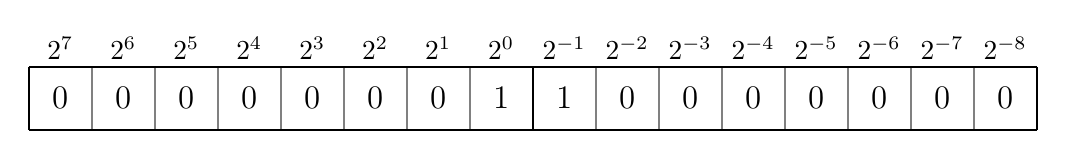
\begin{tikzpicture}[scale=0.8, every node/.style={scale=0.99}]


\colorlet{LighterMark}{black!50}

\foreach \i in {1,...,15}
{
     \draw[thick,LighterMark] (\i,1) -- (\i,0);
}

     \draw[thick,black] (0,1) -- (0,0);
      \draw[thick,black] (8,1) -- (8,0);
      \draw[thick,black] (16,1) -- (16,0);
      
\draw[thick,black] (0,0) -- (16,0);
\draw[thick,black] (0,1) -- (16,1);
 

%\foreach \i[evaluate={\pow=int(7-\i)}] in {0,...,7}
\foreach \i[evaluate={\pow=int(7-\i)}] in {0,...,7}
{
   \node[] at (\i+0.5,1.3){$2^{\pow}$  }  ;
      
         
     
}

%\foreach \i[evaluate={\pow=int((\i-7)*2)}]  in {8,...,15}
\foreach \i[evaluate={\pow=int(\i-7)}]  in {8,...,15}
{
     \node[] at (\i+0.5,1.3){$2^{-\pow}$}  ;
}

\tikzstyle{fontbf} = [font=\large]
\node[fontbf] at (0.5,0.5){0} ;
\node[fontbf] at (1.5,0.5){0};  
\node[fontbf] at (2.5,0.5){0} ; 
\node[fontbf] at (3.5,0.5){0} ;

\node[fontbf] at (4.5,0.5){0} ;
\node[fontbf] at (5.5,0.5){0};  
\node[fontbf] at (6.5,0.5){0} ; 
\node[fontbf] at (7.5,0.5){1} ;

\node[fontbf] at (8.5,0.5){1} ;
\node[fontbf] at (9.5,0.5){0};  
\node[fontbf] at (10.5,0.5){0} ; 
\node[fontbf] at (11.5,0.5){0} ;

\node[fontbf] at (12.5,0.5){0} ;
\node[fontbf] at (13.5,0.5){0};  
\node[fontbf] at (14.5,0.5){0} ; 
\node[fontbf] at (15.5,0.5){0} ;


\end{tikzpicture}

   \caption{1.5} 
\end{figure} 
\par
First shift both operators by 4 bits to the right:\\
\par
\begin{figure}[H]
 \centering
   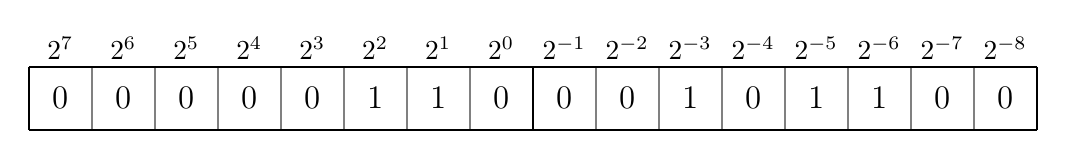
\begin{tikzpicture}[scale=0.8, every node/.style={scale=0.99}]


\colorlet{LighterMark}{black!50}

\foreach \i in {1,...,15}
{
     \draw[thick,LighterMark] (\i,1) -- (\i,0);
}

     \draw[thick,black] (0,1) -- (0,0);
      \draw[thick,black] (8,1) -- (8,0);
      \draw[thick,black] (16,1) -- (16,0);
      
\draw[thick,black] (0,0) -- (16,0);
\draw[thick,black] (0,1) -- (16,1);
 

%\foreach \i[evaluate={\pow=int(7-\i)}] in {0,...,7}
\foreach \i[evaluate={\pow=int(7-\i)}] in {0,...,7}
{
   \node[] at (\i+0.5,1.3){$2^{\pow}$  }  ;
      
         
     
}

%\foreach \i[evaluate={\pow=int((\i-7)*2)}]  in {8,...,15}
\foreach \i[evaluate={\pow=int(\i-7)}]  in {8,...,15}
{
     \node[] at (\i+0.5,1.3){$2^{-\pow}$}  ;
}

\tikzstyle{fontbf} = [font=\large]
\node[fontbf] at (0.5,0.5){0} ;
\node[fontbf] at (1.5,0.5){0};  
\node[fontbf] at (2.5,0.5){0} ; 
\node[fontbf] at (3.5,0.5){0} ;

\node[fontbf] at (4.5,0.5){0} ;
\node[fontbf] at (5.5,0.5){1};  
\node[fontbf] at (6.5,0.5){1} ; 
\node[fontbf] at (7.5,0.5){0} ;

\node[fontbf] at (8.5,0.5){0} ;
\node[fontbf] at (9.5,0.5){0};  
\node[fontbf] at (10.5,0.5){1} ; 
\node[fontbf] at (11.5,0.5){0} ;

\node[fontbf] at (12.5,0.5){1} ;
\node[fontbf] at (13.5,0.5){1};  
\node[fontbf] at (14.5,0.5){0} ; 
\node[fontbf] at (15.5,0.5){0} ;


\end{tikzpicture}

\end{figure} 
\par
\begin{figure}[H]
 \centering
   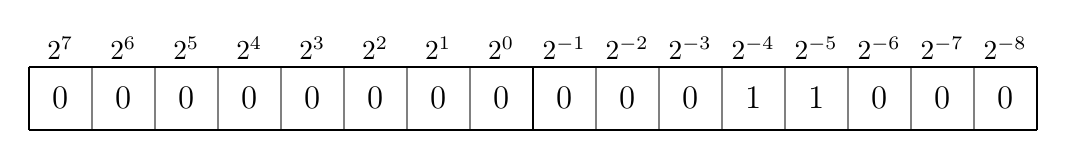
\begin{tikzpicture}[scale=0.8, every node/.style={scale=0.99}]


\colorlet{LighterMark}{black!50}

\foreach \i in {1,...,15}
{
     \draw[thick,LighterMark] (\i,1) -- (\i,0);
}

     \draw[thick,black] (0,1) -- (0,0);
      \draw[thick,black] (8,1) -- (8,0);
      \draw[thick,black] (16,1) -- (16,0);
      
\draw[thick,black] (0,0) -- (16,0);
\draw[thick,black] (0,1) -- (16,1);
 

%\foreach \i[evaluate={\pow=int(7-\i)}] in {0,...,7}
\foreach \i[evaluate={\pow=int(7-\i)}] in {0,...,7}
{
   \node[] at (\i+0.5,1.3){$2^{\pow}$  }  ;
      
         
     
}

%\foreach \i[evaluate={\pow=int((\i-7)*2)}]  in {8,...,15}
\foreach \i[evaluate={\pow=int(\i-7)}]  in {8,...,15}
{
     \node[] at (\i+0.5,1.3){$2^{-\pow}$}  ;
}

\tikzstyle{fontbf} = [font=\large]
\node[fontbf] at (0.5,0.5){0} ;
\node[fontbf] at (1.5,0.5){0};  
\node[fontbf] at (2.5,0.5){0} ; 
\node[fontbf] at (3.5,0.5){0} ;

\node[fontbf] at (4.5,0.5){0} ;
\node[fontbf] at (5.5,0.5){0};  
\node[fontbf] at (6.5,0.5){0} ; 
\node[fontbf] at (7.5,0.5){0} ;

\node[fontbf] at (8.5,0.5){0} ;
\node[fontbf] at (9.5,0.5){0};  
\node[fontbf] at (10.5,0.5){0} ; 
\node[fontbf] at (11.5,0.5){1} ;

\node[fontbf] at (12.5,0.5){1} ;
\node[fontbf] at (13.5,0.5){0};  
\node[fontbf] at (14.5,0.5){0} ; 
\node[fontbf] at (15.5,0.5){0} ;


\end{tikzpicture}

\end{figure} 
\par

Finally multiply them together:

\begin{figure}[H]
 \centering
   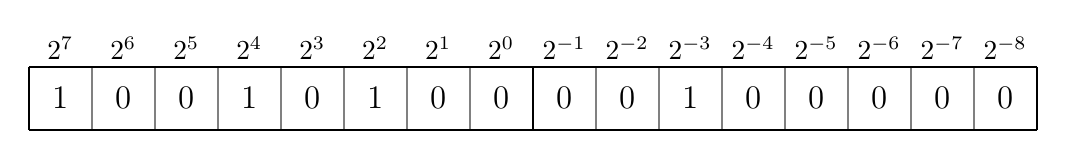
\begin{tikzpicture}[scale=0.8, every node/.style={scale=0.99}]


\colorlet{LighterMark}{black!50}

\foreach \i in {1,...,15}
{
     \draw[thick,LighterMark] (\i,1) -- (\i,0);
}

     \draw[thick,black] (0,1) -- (0,0);
      \draw[thick,black] (8,1) -- (8,0);
      \draw[thick,black] (16,1) -- (16,0);
      
\draw[thick,black] (0,0) -- (16,0);
\draw[thick,black] (0,1) -- (16,1);
 

%\foreach \i[evaluate={\pow=int(7-\i)}] in {0,...,7}
\foreach \i[evaluate={\pow=int(7-\i)}] in {0,...,7}
{
   \node[] at (\i+0.5,1.3){$2^{\pow}$  }  ;
      
         
     
}

%\foreach \i[evaluate={\pow=int((\i-7)*2)}]  in {8,...,15}
\foreach \i[evaluate={\pow=int(\i-7)}]  in {8,...,15}
{
     \node[] at (\i+0.5,1.3){$2^{-\pow}$}  ;
}

\tikzstyle{fontbf} = [font=\large]
\node[fontbf] at (0.5,0.5){1} ;
\node[fontbf] at (1.5,0.5){0};  
\node[fontbf] at (2.5,0.5){0} ; 
\node[fontbf] at (3.5,0.5){1} ;

\node[fontbf] at (4.5,0.5){0} ;
\node[fontbf] at (5.5,0.5){1};  
\node[fontbf] at (6.5,0.5){0} ; 
\node[fontbf] at (7.5,0.5){0} ;

\node[fontbf] at (8.5,0.5){0} ;
\node[fontbf] at (9.5,0.5){0};  
\node[fontbf] at (10.5,0.5){1} ; 
\node[fontbf] at (11.5,0.5){0} ;

\node[fontbf] at (12.5,0.5){0} ;
\node[fontbf] at (13.5,0.5){0};  
\node[fontbf] at (14.5,0.5){0} ; 
\node[fontbf] at (15.5,0.5){0} ;


\end{tikzpicture}

   \caption{98.7539 * 1.5 = 148.125} 
\end{figure} 
$128 + 16 + 4 + 0.125 = 148.125 $\\
\par
Notice that you have to be careful. In the previous example some precision was lost ($ 2^{-8}$ bits disappeared during the $\gg 4$ operation) and an overflow could have occurred (multiplying by 3 instead of 1.5 would have gone past the precision of 8:8).\\
\par
In the source code, all fixed point variables are 32 bits wide and use a special \cw{typedef}.\\
\par
\begin{minipage}{\textwidth}
 \lstinputlisting[language=C]{code/fixed.c}
 \end{minipage}
\par
Not all \cw{fixed} are the same. Some are \cw{16:16}, some are \cw{24:8} and operations such as multiplication can be implemented differently. It can be fairly complicated for tweaked \cw{fixed} where the leftmost bit stores the sign:\\
\par
\begin{minipage}{\textwidth}
 \lstinputlisting[language=C,morekeywords={asm,fixed}]{code/FixedByFrac.c}
 \end{minipage}
\par
And much easier when the engine knows two \cw{fixed} are the same sign:\\

\par
\begin{minipage}{\textwidth}
 \lstinputlisting[language=C]{code/fixed_mul.c}
 \end{minipage}
\par

 \textbf{\underline{Trivia :}}  Fixed Point Arithmetic usage was not limited to PC gaming. Many game consoles manufactured in the 90s and later did not feature floating point units in order to reduce production cost and maximize CPU pipeline throughout. Sony's original PlayStation (1994) and Sega's Saturn (1994) are examples.
 

 
 


\subsubsection{Coordinate System}
With the CPU \cw{float}/\cw{int} problem out of the way, it is time to study how a ray is cast. The coordinate system finds its origin in the upper left. A map is a grid of 64 by 64 blocks. 
\begin{figure}[H]
  \centering
 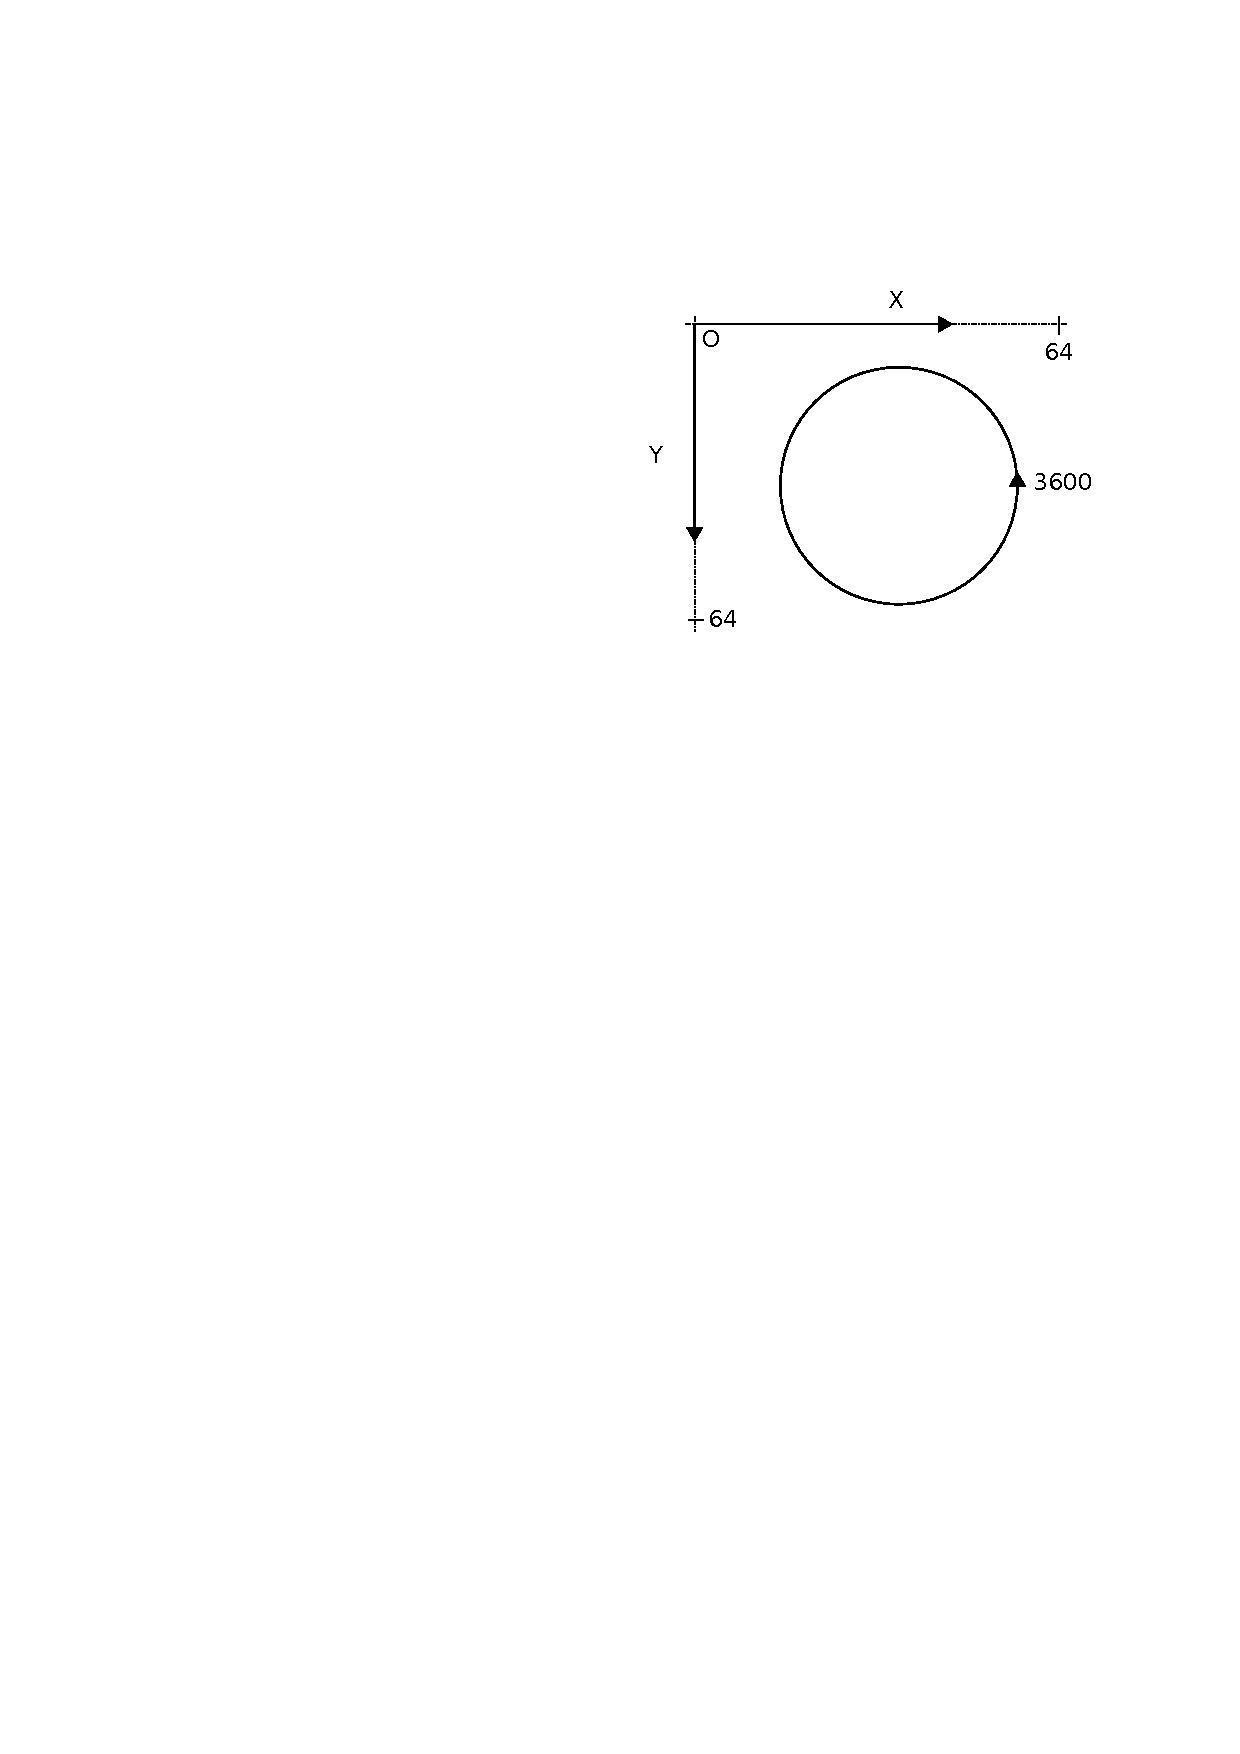
\includegraphics[width=.8\textwidth]{imgs/drawings/coo_sys.pdf}
\end{figure}
\par
Since one block is 8 feet, maps can be 512 feet wide and tall. Fixed point variables are used all over the place. Column heights are 29:3. Player position is 16:16. Angles however are \cw{int}s representing tenths of degrees with a range [0, 3600].

















\subsubsection{Square World and Ray Casting}
Drawing the walls is all about determining what is visible, what is not, and what is in front of what. Michael Abrash's view on the topic tells it all:\\
\par
\begin{fancyquotes}
I want to talk about what is, in my book, the toughest 3-D problem of all, visible surface determination (drawing the proper surface at each pixel), and its close relative, culling (discarding non-visible polygons as quickly as possible, a way of accelerating visible surface determination). In the interests of brevity, I'll use the abbreviation VSD to mean both visible surface determination and culling from now on.
 \bigskip \\
Why do I think VSD is the toughest 3-D challenge? Although rasterization issues such as texture mapping are fascinating and important, they are tasks of relatively finite scope, and are being moved into hardware as 3-D accelerators appear; also, they only scale with increases in screen resolution, which are relatively modest.
 \bigskip \\
In contrast, VSD is an open-ended problem, and there are dozens of approaches currently in use. Even more significantly, the performance of VSD, done in an unsophisticated fashion, scales directly with scene complexity, which tends to increase as a square or cube function, so this very rapidly becomes the limiting factor in doing realistic worlds. I expect VSD increasingly to be the dominant issue in realtime PC 3-D over the next few years, as 3-D worlds become increasingly detailed.
 \bigskip \\
\textbf{Michael Abrash - Graphics Programming Black Book}
 \end{fancyquotes}\\
\par
\begin{wrapfigure}[17]{r}{0.45\textwidth} 
\vspace{-10pt}
\scaledimage{0.45}{gpbb.png} 
\end{wrapfigure} 
\bu{Trivia: } In the early 90s, Michael Abrash writings were one of the rare source of high quality information when it came to Computer Graphics and Assembly programming.\\
\par
He published two highly regarded books ("Zen of Assembly Language" in 1990 and "Zen of Code Optimization" in 1994) but it is though his column "Ramblings in Realtime" published monthly in Dr. Dobb's Journal that he achieved notoriety.
 \\
\par
 In 1997 most of Michael Abrash work plus new articles about Quake engine were compiled into the "Graphics Programming Black Book". The title and dimension of this book are an homage to Mr Abrash's masterpiece.





\begin{figure}[H]
\centering
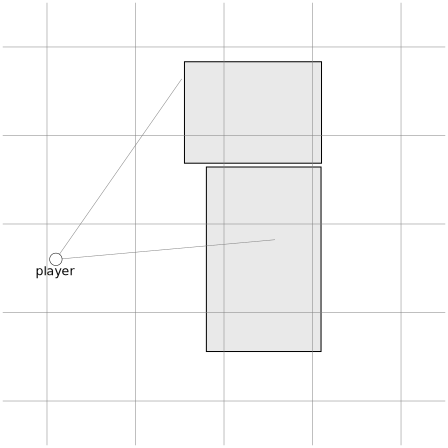
\includegraphics[width=\textwidth]{imgs/drawings/casting_a_ray/situation.pdf} 
\end{figure}
VSD is not only complicated to do right, it is also hard to do fast. It is easy to understand with a small example where objects are free form with no alignment, as follows. In a world with no constraints, it is difficult to find the intersection of a ray with an object.\\
\par
In the example above, a valid approach would be to iterate over all objects in the world and perform ray marching, which consists of checking if a ray intersects objects at a regular interval. However, this is very CPU intensive and would not be fast enough with fixed point. Not to mention some objects could slip between the regular intervals, making VSD inaccurate.
\begin{figure}[H]
\centering
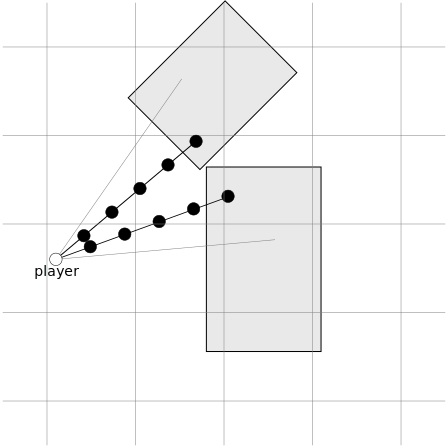
\includegraphics[width=\textwidth]{imgs/drawings/casting_a_ray/unaligned.pdf}
 \caption{Ray marching in action.}
\end{figure}


In a world with some constraints the problem becomes much simpler. If a map is made of aligned square blocks evenly distributed across a grid, a solution yielding 100\% accuracy and low runtime overhead is to check for 'hits` only when a ray crosses the grid.\\
\par
 This was the choice made for Wolfenstein 3D, and explains why the game can only draw perpendicular walls of 8 feet by 8 feet by 8 feet.\\
\par
\begin{figure}[H]
\centering
\includegraphics[width=\textwidth]{imgs/drawings/casting_a_ray/fixed.pdf}
 \caption{Raycasting with a grid.}
\end{figure}
\par
These constraints enable a variant of the DDA algorithm\footnote{Digital differential analyzer.}, which is a fast and accurate way to detect where a ray hits a wall on the map.
\par
\begin{fancyquotes}
\par
Much was made about the "ray casting" used in Wolfenstein, but the real reason for it was that I had a lot of trouble with wall-span rendering in Catacomb 3D.  C3D (and Hovertank 3D before that) shipped with various graphics glitches that you could get in some combinations of map block configurations, position, and viewing angle.  Some were due to fixed point precision issues not being handled optimally, and some were due to clipping and culling issues that I didn't really get a handle on until a couple years later.  In any case, they bothered me a lot.  Spurious graphics glitches do a lot of harm to the sense of immersion in a game, and I very much wanted Id games to feel "rock solid".
 \bigskip \\
There was a clear performance cost to it - doing 320 traces through a tile map and treating each column independently is much slower than looping through a few long wall segments.  However, the resulting code was small and very regular compared to the hairball of my wall span renderers, and it did deliver the rock-solid feel I wanted.
 \bigskip \\
If you made extremely jagged block maps that would turn into many dozen independent wall segments, the ray casting could start to look like a good performance choice, but few scenes were even close to that.  This is exactly the same ray tracing versus rasterization performance tradeoff that is still being made today, but now it is "how many tens of millions of triangles per frame to ray tracing break-even" instead of "how many dozen wall segments".
 \bigskip \\
\textbf{John Carmack - Programmer}
 \end{fancyquotes}\\
\par


\begin{wrapfigure}[14]{r}{0.45\textwidth} 
\vspace{-10pt}
\scaledimage{0.45}{e1m1.png} 
\end{wrapfigure} 
\bu{Trivia :} The cost of raycasting would end up being too much for the tiny 5A22 CPU when porting Wolfenstein 3D to Super Nintendo.\\
\par
 The first version of the port reached an unacceptably low framerate which threatened the port.\\
 \par
 id was faced with the choice of overcoming the problems with "wall-span rendering" or cancel the SNES version altogether. He ended up using Binary Space Partitioning for the first time, a technique he later used for Doom.

 




\begin{figure}[H]
  \centering
 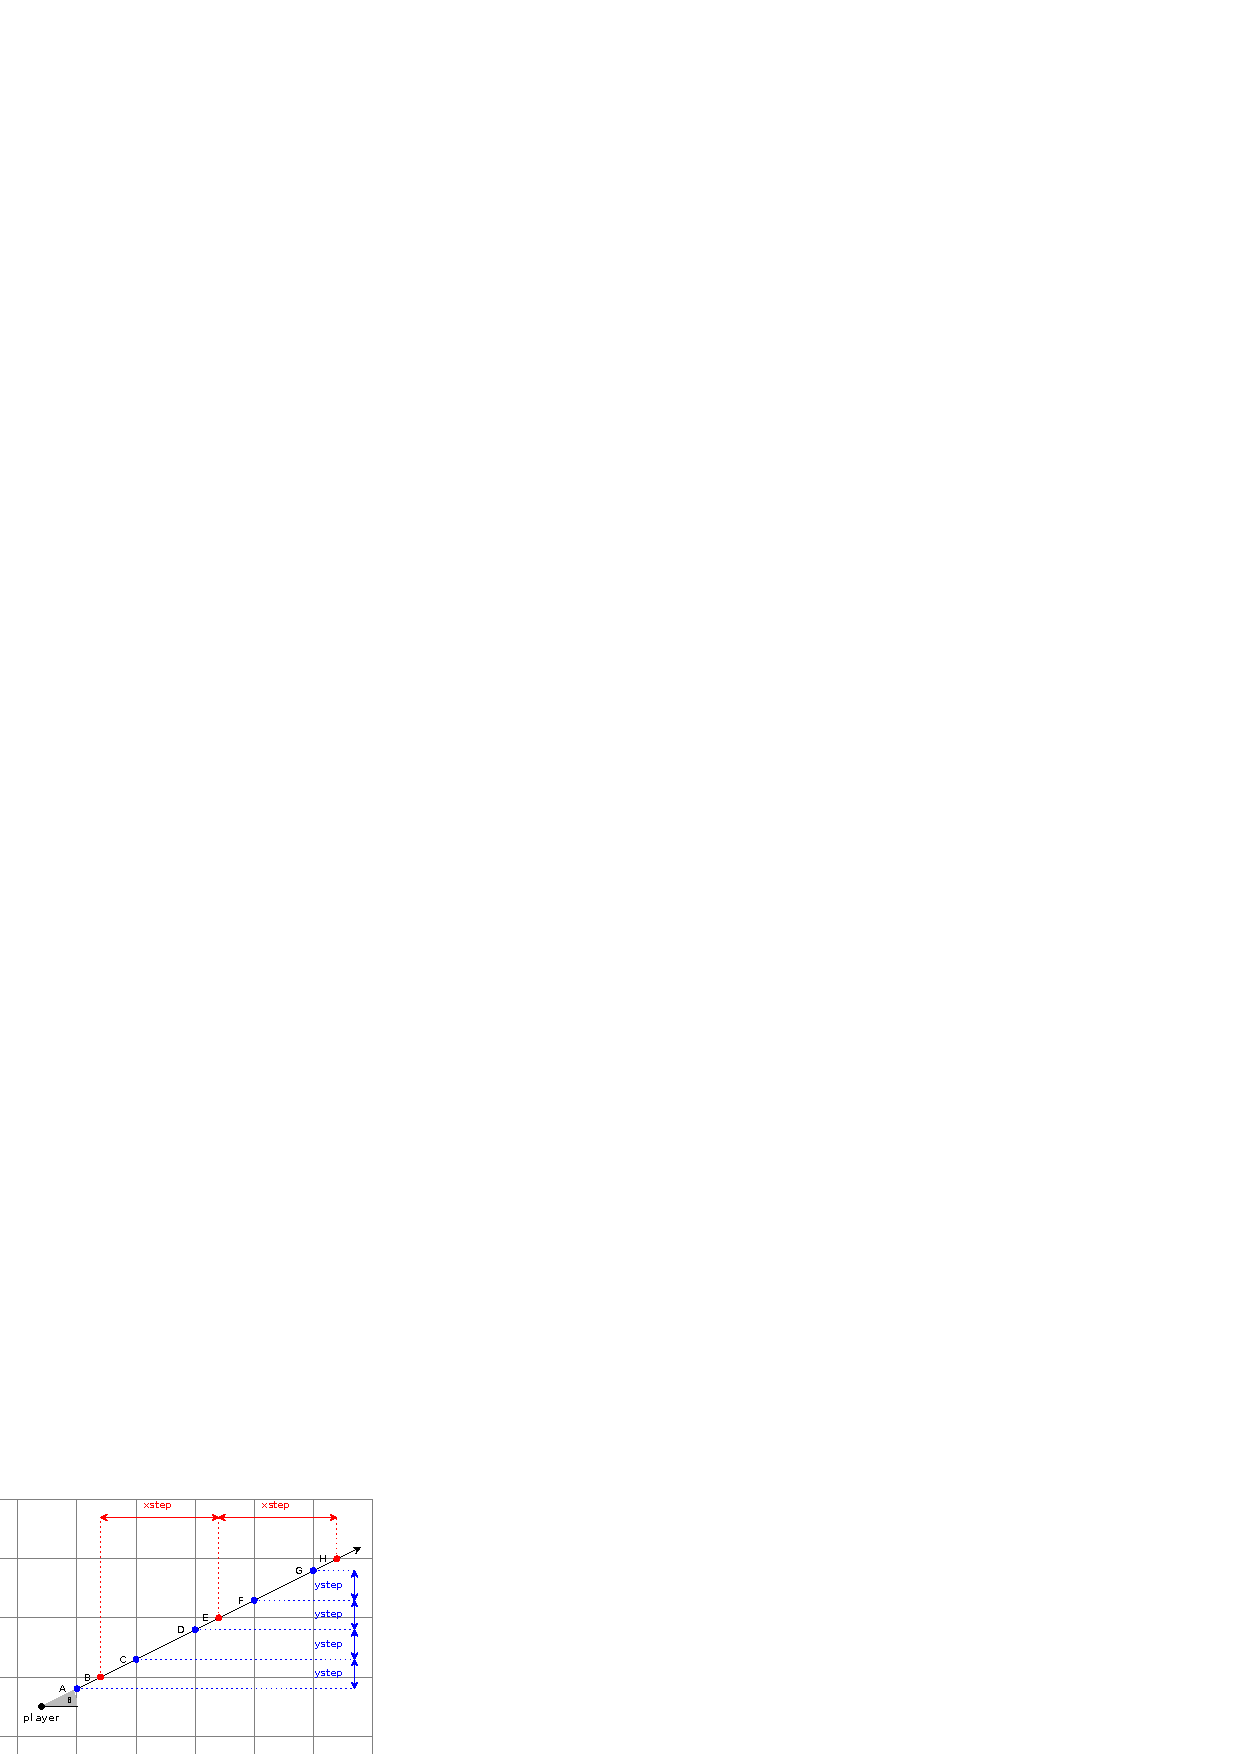
\includegraphics[width=\textwidth]{imgs/drawings/dda.pdf}
\end{figure}
\par


DDA is so fast because once the first intersection of a ray with an axis is known (A for Y axis and B for X axis), all subsequent intersections' coordinates are two additions away.
\par


\begin{equation*}
    \scalebox{1.3}{
$C = (X_{A} +1, Y_{A} + ystep)$\\
}
\end{equation*}
\begin{equation*}
    \scalebox{1.3}{
$D = (X_{C} +1, Y_{C} + ystep)$\\
}
\end{equation*}
\begin{equation*}
    \scalebox{1.3}{
$F = (X_{D} +1, Y_{D} + ystep)$\\
}
\end{equation*}
\begin{equation*}
    \scalebox{1.3}{
$G = (X_{F} +1, Y_{F} + ystep)$\\
}
\end{equation*}


\par
Similarly, for the vertical intersections:\\
  \begin{equation*}
    \scalebox{1.3}{

$E = (X_{B} + xstep, Y_{B} + 1)$\\
}
\end{equation*}
  \begin{equation*}
    \scalebox{1.3}{
$D = (X_{E} + xstep, Y_{E} + 1)$\\
}
\end{equation*}\\
\par
Note that $ystep$ and $xstep$ are simple lookups into the \cw{tan} array since $xstep=tan(\theta)$ and $ystep=tan(90-\theta)$ where $\theta$ is the angle of the ray in map coordinates\footnote{A visual reminder of how the unit circle works can be found on page \pageref{unit_circle}.}.\\
\par
\begin{figure}[H]
  \centering
 \fullimage{e1m1.png}
 \label{mape1m1}
 \caption{The legendary E1M1. Player is the green arrow at the bottom.}
\end{figure}


\subsubsection{Call Apogee}
With maps being quick and easy to draw, a contest was planned. Players who found a special item in a particularly difficult to access place in the game were instructed to call the publisher (Apogee).\\
\par The maze is located in E2M8. Behind a forest of push walls (white squares) and angry bosses (blue circles), the player finally encounters an strange sign (the red triangle).


\begin{figure}[H]
  \centering
 \fullimage{e2m8.png}
 \caption{E2M8 maze.}
\end{figure}
\par
\begin{wrapfigure}[8]{r}{0.4\textwidth}
\vspace{-10pt}
\scaledimage{0.4}{call_apogee.png} 
\end{wrapfigure}
However, as players reverse engineered the map format and cheat sites emerged, the contest was called off. The sign was replaced with a skeleton in all games shipped in 1992.\\
\par
In the previous map, notice there are no push walls leading to the red triangle; the room is sealed.\\
\begin{fancyquotes}
"Call Apogee and say Aardwolf."  It's a sign that to this day is something
that I get asked about a lot.  This is a sign that appears on a wall in a
particularly nasty maze in Episode 2 Level 8 of Wolfenstein 3D.  The sign
was to be the goal in a contest Apogee was going to have, but almost
immediately after the game's release, a large amount of cheat and mapping
programs were released.  With these programs running around, we felt that
it would have been unfair to have the contest and award a prize.  The sign
was still left in the game, but in hindsight, probably should have been
taken out.  To this day, Apogee gets letters and phone calls and asking
what Aardwolf is, frequently with the question, "Has anyone seen this yet?"\\
\\
Also, in a somewhat related issue, letters were shown after the highest score
in the score table in some revisions of the game.  These letters were to be
part of another contest that got scrapped before it got started, where we were
going to have people call in with their scores and tell us the code; we'd then
be able to verify their score.  However, with the cheat programs out there,
this got scrapped too.\\
\\
Basically, "Aardwolf" and the letters mean nothing now.\\
\\
\textbf{Joe Siegler - Past Pioneers of the Shareware Revolution}
\end{fancyquotes}
\par
\bigskip
\bu{Trivia :} What is Aardwolf? A maned striped mammal (Proteles cristatus) of southern and eastern Africa that resembles a hyena and feeds chiefly on carrion and insects. It was the mascot of id, appearing on Tom's Gotta Lists and the Commander Keen 6 Hint Sheet.\\
\par

 \begin{fancyquotes}
The reason for "aardwolf" was that it was the first image file in the NeXT dictionary on all of our NeXTStations.
\bigskip \\
\textbf{John Carmack - Programmer}
 \end{fancyquotes}













 
 
 
 
 
 
 
 
\subsubsection{Raycasting: DDA Algorithm}
The DDA intersection algorithm is implemented in a fully-handcrafted 740 lines of assembly routine: \cw{AsmRefresh}. It is represented here in pseudo-C for readability. It consists of two while loops (one each for vertical and horizontal intersections) ping-ponging with each other via goto. It is highly unorthodox and super efficient.\\
\par



\begin{minipage}{\textwidth}
\lstinputlisting[language=C]{code/flipflop.c}
\end{minipage}
This implementation results in many \cw{jmp} instructions. These would kill the icache and empty the pipeline on a modern CPU. But on an architecture with a small pipeline and no i-cache such as the 386 it is not a frame killer.\\
\par
This part of the code relies heavily on unit circle principles. As we need to know how much to go vertically when advancing on the X axis and how much to go horizontally when advancing on the Y axis, the \cw{tan} function is especially useful. This is easier to understand with the unit circle drawn (circle radius $r$ is equal to 1).
\label{unit_circle}
\scaleddrawing{0.5}{unit_circle}{Unit circle}
\par
When advancing 1 on the X axis, the ray moves up $tan(\theta)$ on the Y axis. The reciprocal is calculated as follows: move 1 on Y axis, move $tan(90-\theta)$ on X axis. To accelerate \cw{cos}, \cw{sin} and \cw{tan} calculations, the engine uses lookup table. See \ref{cossintable} "\nameref{cossintable}" on page \pageref{cossintable}.




















\subsubsection{High School Math}
Before proceeding to the next section (describing what is done with the distance from the player to the wall), here is a short refresher on a piece of high school math which forms the foundation of most calculations in the engine: SOH-CAH-TOA.\\



\par
\scaleddrawing{0.6}{soh-cah-toa}{Unit circle}
\par
 \begin{fancyquotes}
  I'm no super mathematician-- I learned high school math well enough to solve real world problems with it.\\
 \par
\textbf{John Carmack - Programmer}
 \end{fancyquotes}
\par



This drawing is all the math you need to understand the fish eye correction and coordinate projections used to place objects (player, enemies, items) and calculate sound locations.\\






















\subsubsection{Calculating Column Heights}
Once the intersection between a ray and a wall is found from coordinate (\cw{viewx}, \cw{viewy}) to (\cw{xintercept}, \cw{yintercept}), it is time to calculate how tall the column of pixels for this ray should be. This happens in the function \cw{CalcHeight}.\\

\begin{minipage}{\textwidth}
\lstinputlisting[language=C]{code/CalcHeight.c}
\end{minipage}

The code is not what one would expect. The raycasting algorithm is supposed to cast a ray for each pixel column and use the distance \codeword{d} to infer the column's height on screen. So it would have made sense to see a formula like:
\begin{figure}[H]
  \centering
  \begin{equation*}
    \scalebox{1.3}{
$ d = \sqrt{dx^2 + dy^2}$ 
 }
  \end{equation*}
\end{figure}
Instead the code looks like it is doing: 
\begin{figure}[H]
  \centering
  \begin{equation*}
    \scalebox{1.3}{
$d = dx * \cos(\alpha) - dy * \sin(\alpha) $
 }
  \end{equation*}
\end{figure}
Something is fishy here. Let's explain with an example.\\
\par
\begin{figure}[H]
\centering
 %\documentclass[tikz,border=2pt,png]{standalone}
%\usepackage{tkz-euclide}
%\usetkzobj{all}
%\begin{document}
\begin{tikzpicture}[scale=2.0]

\coordinate(origin) at (0,0)[label=below:view] {};
\coordinate(yaxis) at (0,6.5){};
\coordinate(xaxis) at (6,0) {};
\coordinate(angle) at (30:3);
\coordinate(intercept) at (3,5) {};

\node[below left] (orign) {viewpoint};
\node[below right] (_XX) at (intercept) {intercept};

% AXIS
%\draw[->,draw=black,>=stealth] (origin)  -- (xaxis) ;
%\draw[->,draw=black,>=stealth] (origin)  -- (yaxis) ;
%\draw[draw=black] (origin)  -- (0,-0.5) ;
%\draw[draw=black] (origin)  -- (-0.5,0) ;

% WALL
\fill[black!20!white, draw=black] (2,5) rectangle (4,7);
%\fill[black!20!white, draw=black] (4,5) rectangle (6,7);
%\fill[black!20!white, draw=black] (4,3) rectangle (6,5);


\fill (intercept) circle (2pt);


\draw[->,draw=gray,>=stealth] (origin)  -- (angle) ;

\coordinate (dx) at ($(origin)!(intercept)!(xaxis)$);
\draw[draw=gray,>=stealth,dashed] (origin) -- node[below] {dx} (dx);
\draw[draw=gray,>=stealth,dashed] (intercept) -- node[right] {dy}(dx);

\tkzMarkAngle[fill= gray,size=0.8cm,opacity=.2](xaxis,origin,angle)
\tkzLabelAngle[pos = 0.6](xaxis,origin,angle){$\alpha$}

\fill[fill=black] (origin) circle (2pt);

\draw[] (origin) -- node[below] {d} ++(intercept) ;

%\draw[] 


\end{tikzpicture}
%\end{document}
 \caption{Raycasting using distance d} \label{fig:Raycasting2}
\end{figure}

In this drawing the player is located at \cw{viewpoint} with a view angle \begin{math}\alpha\end{math}. A ray has been cast from \cw{viewpoint} and it hit a wall at \cw{intercept}. The distance \codeword{d} is a straight line between the player's point of view and the location where the ray hit the wall. $d$ can be obtained with $d = \sqrt{dx^2 + dy^2}$. Repeated for all rays, such an algorithm would result in a "fisheye effect".









\begin{minipage}{\textwidth}

    \begin{figure}[H]
    \centering
    \vspace{-10pt}
      \fullimage{fish_eye/bad_mild.png}
     \caption{Fish eye effect: Mild}. \label{fig:mips}
     \end{figure} 


    \begin{minipage}{.4\textwidth}
    This visual artifact happens because the straight distance from the player to the wall is not constant. Walls are further away on the side of the screen and therefore represented smaller.\\
    \par
    To demonstrate the fish eye distortion, here are three screenshots from a modified version of the engine. It was altered to use direct distance \cw{d} instead of "something else" to calculate column heights. At first from a distance of 32 feet, the distortion is barely noticeable.\\
     \end{minipage}
    \begin{minipage}{.6\textwidth}
    \begin{figure}[H]
      \begin{flushright}
     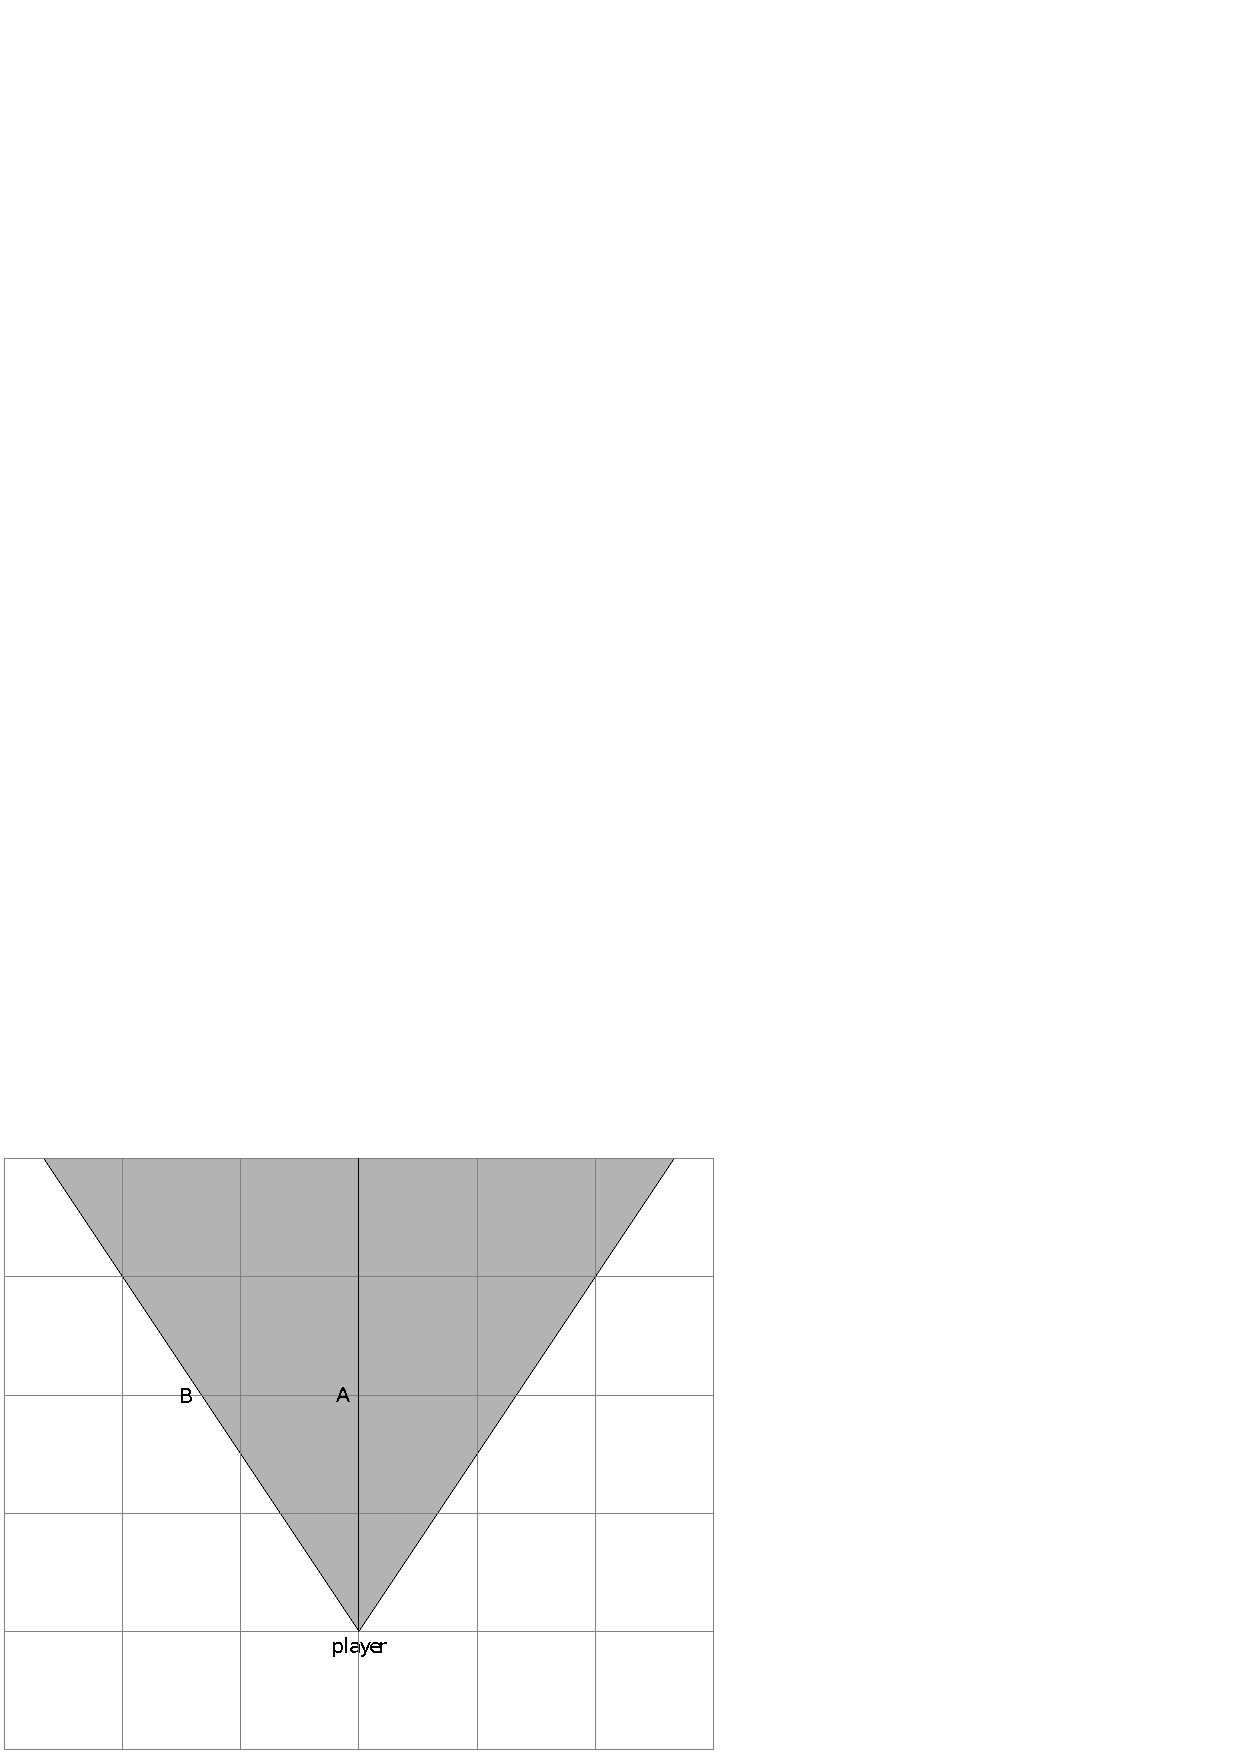
\includegraphics[width=.9\textwidth]{imgs/drawings/fish_eye/top_view_far.pdf}
       \end{flushright}
    \end{figure}
    \end{minipage}
\end{minipage}
\par



\begin{minipage}{\textwidth}
\begin{figure}[H]
\centering
  \fullimage{fish_eye/bad_ok.png}
 \caption{Fish eye effect: Bad} \label{fig:mips}
 \end{figure}
\begin{minipage}{.4\textwidth}
From a distance of 24 feet, the distortion cannot be ignored and the problem is clear.\\
\par
Note that even though the player is getting closer to the wall, the ratio of A to B remains the same. Only the absolute difference in pixel height when the column is rendered on screen is increasing.
 \end{minipage}
\begin{minipage}{.6\textwidth}
\begin{figure}[H]
  \begin{flushright}
 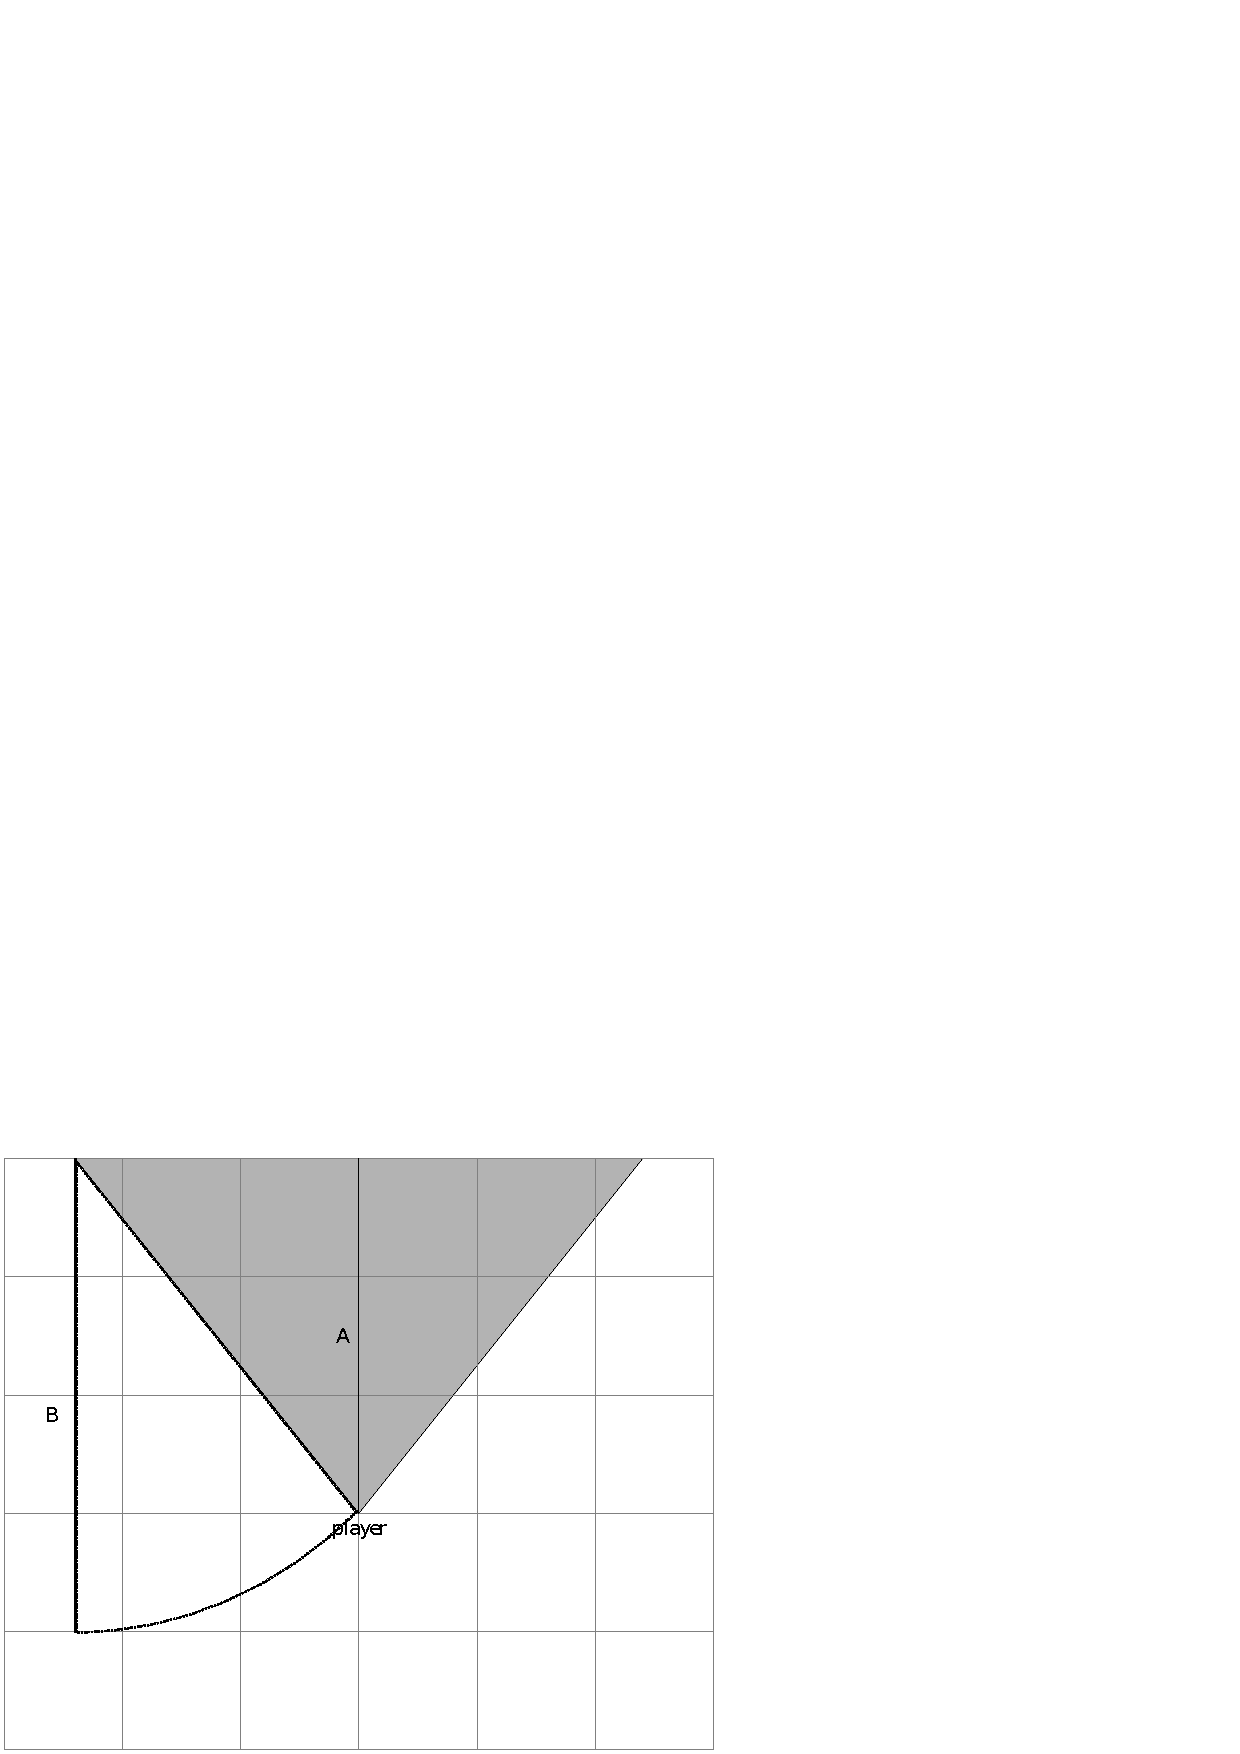
\includegraphics[width=.9\textwidth]{imgs/drawings/fish_eye/top_view_middle.pdf}
 \end{flushright}
\end{figure}
\end{minipage}
\end{minipage}




\begin{minipage}{\textwidth}
 \begin{figure}[H]
\centering
  \fullimage{fish_eye/bad_bad.png}
 \caption{Fish eye effect: AAAAARGH} \label{fig:mips}
 \end{figure}
 

\begin{minipage}{.4\textwidth}
At 12 feet, the distortion is straight up unpleasant with a claustrophobic touch.\\
\par
To avoid this distortion and produce a more pleasant rendition, what must be used is not the direct distance \cw{d} but distance projected on the camera plane (perpendicular to the view direction (\cw{z})).
 \end{minipage}
\begin{minipage}{.6\textwidth}
 \begin{figure}[H]
  \begin{flushright}
  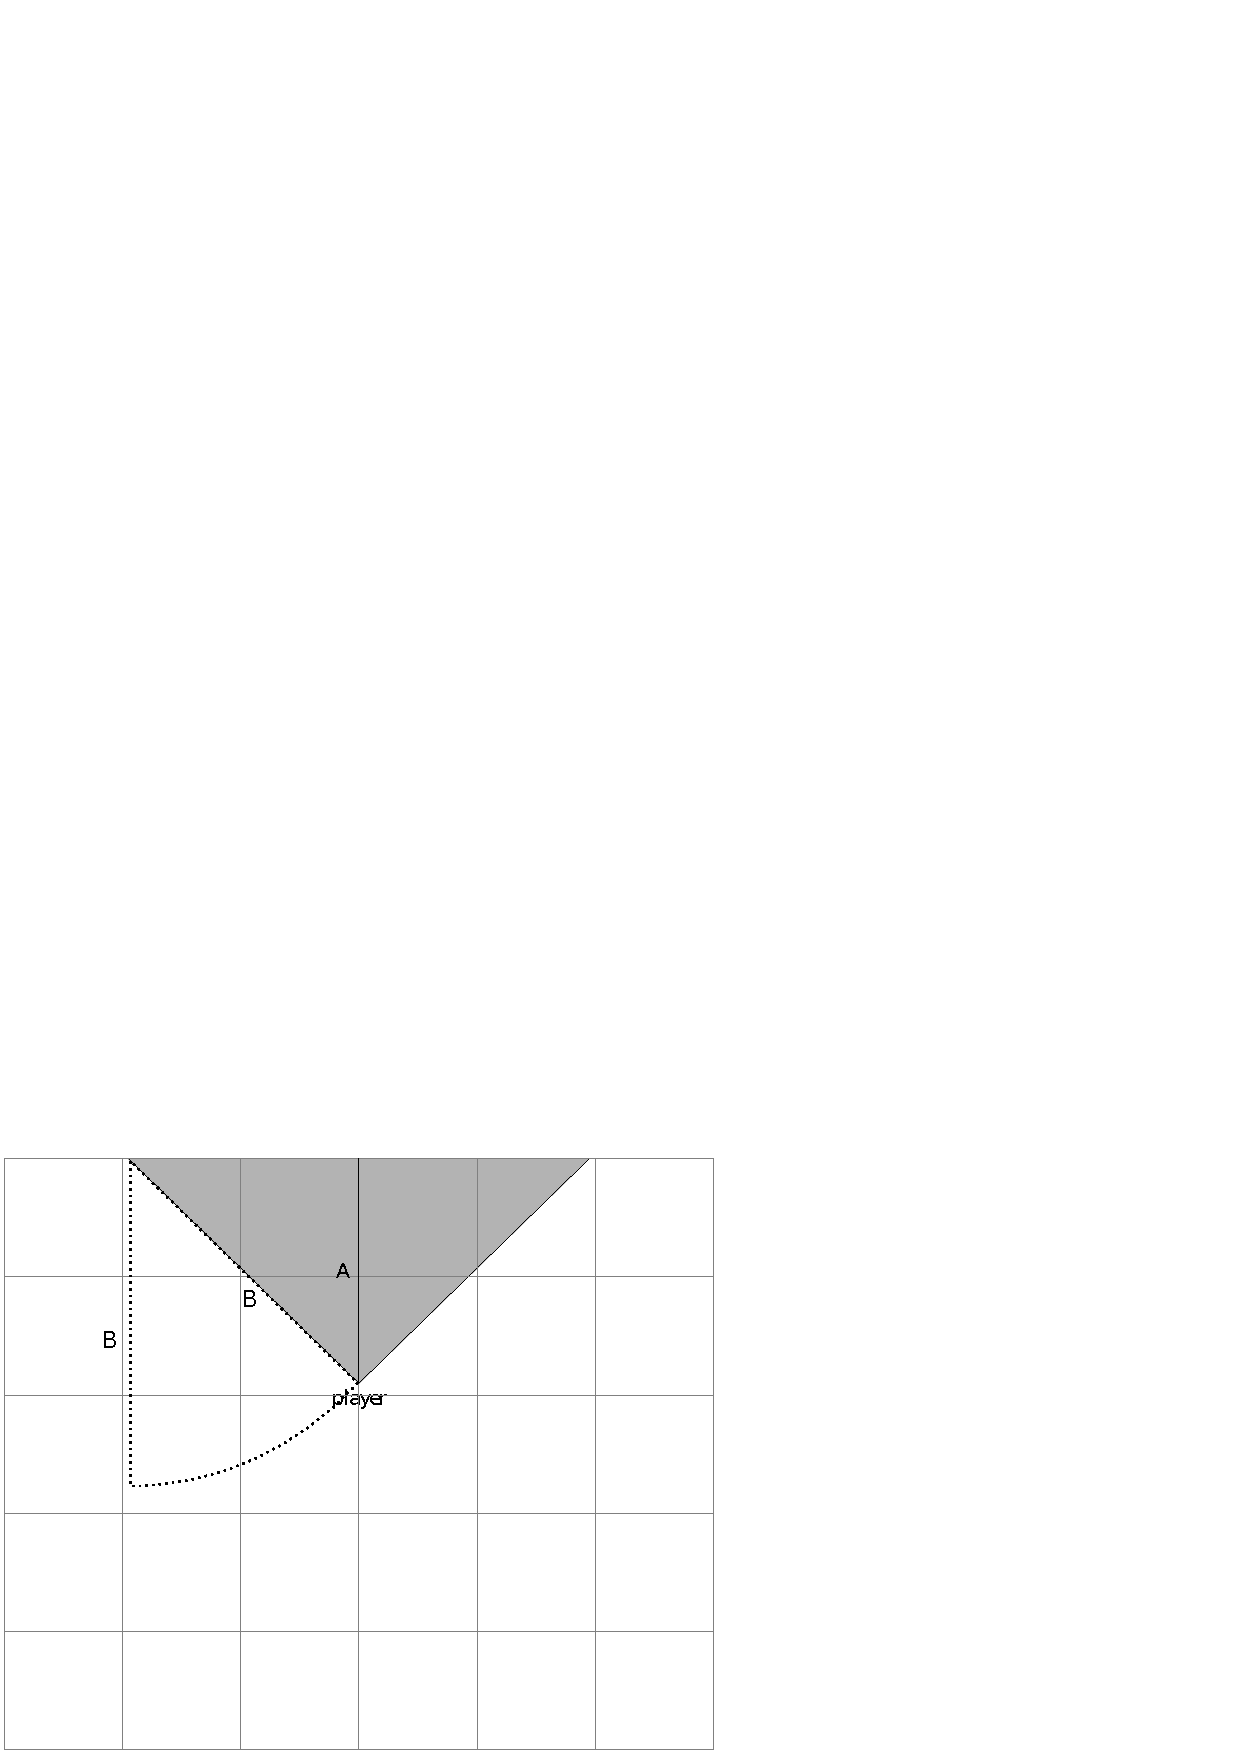
\includegraphics[width=.9\textwidth]{imgs/drawings/fish_eye/top_view_close.pdf}
 \end{flushright}
\end{figure}
 \end{minipage}
\end{minipage}
\par



\begin{figure}[H]

 %\documentclass[tikz,border=2pt,png]{standalone}
%\usepackage{tkz-euclide}
%\usetkzobj{all}
%\begin{document}
\begin{tikzpicture}[scale=2.0]

\coordinate(origin) at (0,0)[label=below:view] {};
\coordinate(yaxis) at (0,6.5){};
\coordinate(xaxis) at (6,0) {};
\coordinate(angle) at (30:3);
\coordinate(intercept) at (3,5) {};

\node[below left] (orign) {viewpoint};
\node[below right] (_XX) at (intercept) {intercept};

% plan
\coordinate(planA) at (120:5);
\coordinate(planB) at (-60:1);
\draw[draw=gray,dashed] (planA) -- (planB);
% AXIS
%\draw[->,draw=black,>=stealth] (origin)  -- (xaxis) ;
%\draw[->,draw=black,>=stealth] (origin)  -- (yaxis) ;
%\draw[draw=black] (origin)  -- (0,-0.5) ;
%\draw[draw=black] (origin)  -- (-0.5,0) ;

% WALL
\fill[black!20!white, draw=black] (2,5) rectangle (4,7);
%\fill[black!20!white, draw=black] (4,5) rectangle (6,7);
%\fill[black!20!white, draw=black] (4,3) rectangle (6,5);

% projected intercept
\coordinate (proj_intercept) at ($(planA)!(intercept)!(planB)$);
\draw[draw=black] (proj_intercept) -- node[above] {z} (intercept);

\tkzMarkRightAngle(intercept,proj_intercept,origin);
\tkzMarkRightAngle(angle,origin,proj_intercept);

\fill (intercept) circle (2pt);

% Angle
\draw[->,draw=gray,>=stealth] (origin)  -- (angle) ;

\coordinate (dx) at ($(origin)!(intercept)!(xaxis)$);
% DX and DY
\draw[draw=gray,>=stealth,dashed] (origin) -- node[below] {dx} (dx);
\draw[draw=gray,>=stealth,dashed] (intercept) -- node[right] {dy}(dx);

\tkzMarkAngle[fill= gray,size=0.8cm,opacity=.2](xaxis,origin,angle)
\tkzLabelAngle[pos = 0.6](xaxis,origin,angle){$\alpha$}

\fill[fill=black] (origin) circle (2pt);

% D libe
\draw[] (origin) -- node[below] {d} ++(intercept) ;

%\draw[] 


\end{tikzpicture}
%\end{document}
\label{fig:Raycasting2}
 \caption{Direct distance \cw{d} and projected distance \cw{z}.}
\end{figure}

This projection (z) is mathematically hard to calculate in one go (especially with fixed point). The trick is to break it down into two components and use the mnemonic SOH-CAH-TOA.\\


\begin{figure}[H]
\centering
 %\documentclass[tikz,border=2pt,png]{standalone}
%\usepackage{tkz-euclide}
%\usetkzobj{all}
%\begin{document}
\begin{tikzpicture}[scale=2.0]

\coordinate(origin) at (0,0)[label=below:view] {};
\coordinate(yaxis) at (0,6.5){};
\coordinate(xaxis) at (6,0) {};
\coordinate(angle) at (30:3);
\coordinate(intercept) at (3,5) {};

\node[below left] (orign) {viewpoint};
\node[below right] (_XX) at (intercept) {intercept};

% plan
\coordinate(planA) at (120:5);
\coordinate(planB) at (-60:1);
\draw[draw=gray,dashed] (planA) -- (planB);
% AXIS
%\draw[->,draw=black,>=stealth] (origin)  -- (xaxis) ;
%\draw[->,draw=black,>=stealth] (origin)  -- (yaxis) ;
%\draw[draw=black] (origin)  -- (0,-0.5) ;
%\draw[draw=black] (origin)  -- (-0.5,0) ;

% WALL
\fill[black!20!white, draw=black] (2,5) rectangle (4,7);
%\fill[black!20!white, draw=black] (4,5) rectangle (6,7);
%\fill[black!20!white, draw=black] (4,3) rectangle (6,5);

% projected intercept
\coordinate (proj_intercept) at ($(planA)!(intercept)!(planB)$);
\draw[draw=gray,dashed] (proj_intercept) -- node[above] {} (intercept);

\tkzMarkRightAngle[draw=gray](intercept,proj_intercept,origin);
\tkzMarkRightAngle[draw=gray](angle,origin,proj_intercept);

\fill (intercept) circle (2pt);

% Angle
%\draw[->,draw=gray,>=stealth] (origin)  -- (angle) ;

\coordinate (dx) at ($(origin)!(intercept)!(xaxis)$);
% DX and DY
\draw[draw=gray,>=stealth,dashed] (origin) -- node[below] {dx} (dx);
\draw[draw=gray,>=stealth,dashed] (intercept) -- node[right] {dy}(dx);

\tkzMarkAngle[fill= gray,size=0.8cm,opacity=.2](xaxis,origin,angle)
\tkzLabelAngle[pos = 0.6](xaxis,origin,angle){$\alpha$}

\fill[fill=black] (origin) circle (2pt);

\coordinate (A) at ($(origin)!(dx)!(angle)$);
\draw[] (origin)  -- node[below] {A} (A) ;

\coordinate (B) at ($(proj_intercept)!(dx)!(intercept)$);
\draw[] (intercept)  -- node[above] {B} (B) ;

\draw[draw=gray,dashed] (dx) -- (B) ;

\fill (A) circle (2pt);
\fill (B) circle (2pt);

\tkzMarkAngle[fill= gray,size=0.8cm,opacity=.2](intercept,dx,A)
\tkzLabelAngle[pos = 0.6](intercept,dx,A){$\alpha$}

\end{tikzpicture}
%\end{document}
 \caption{Projected distance \cw{z} it calculated via two sub-components.}
\end{figure}
Using CAH gives $A = dx * \cos(\alpha)$ and SOH gives $B = dy * \sin(\alpha) $.\\
\pagebreak

Adding them together becomes:
\par
\begin{figure}[H]
  \centering
  \begin{equation*}
    \scalebox{1.3}{
$z = A + B = dx * \cos(\alpha) + dy * \sin(\alpha) $. 
 }
  \end{equation*}
\end{figure}
Since dx and dy are not distances but vectors (with a sign) the equation becomes: 


\begin{figure}[H]
  \centering
  \begin{equation*}
    \scalebox{1.3}{
$z = A + B = dx * \cos(-\alpha) + dy * \sin(-\alpha) $ 
 }
  \end{equation*}
\end{figure}
which simplified becomes: 

\begin{figure}[H]
  \centering
  \begin{equation*}
    \scalebox{1.3}{
$z = A + B = dx * \cos(\alpha) - dy * \sin(\alpha) $
 }
  \end{equation*}
\end{figure}
\par
For people who like equations, the overall operation can be seen as the multiplication of a rotation matrix with the vector intercept (dx,dy). It would rotate coordinates from map space to player space (where axis orientation is dictated by the player view angle) as show in figure \ref{spaces2}. \label{rotatematrix}
\begin{figure}[H]
  \centering
  \begin{equation*}
    \scalebox{1.3}{
    $
      \begin{bmatrix} 
        \cos(\alpha) & -\sin(\alpha) \\ 
        \sin(\alpha) & \cos(\alpha) 
      \end{bmatrix} 
       *
      \begin{bmatrix} 
        dx \\ 
        dy 
      \end{bmatrix}
       =
      \begin{bmatrix} 
        dx*\cos(\alpha) - dy*\sin(\alpha) \\ 
        dx*\sin(\alpha) + dy*\cos(\alpha) 
      \end{bmatrix} 
      $
    }
  \end{equation*}
\end{figure}
\par
I personally find the graphic explanation with SOH-CAH-TOA clearer.\\
\par
\subsection{Fisheye Effect Corrected}
This correction is enough to give pleasant straight lines for the walls. To demonstrate the difference, pages \pageref{fish_eye_corrected} and page \pageref{wolf3d_7_fullframe} show two versions of the same scene next to each other. First uncorrected (with fisheye) and then with projected distance \cw{z} instead of direct distance \cw{d}.\\
\par
\pagebreak

\par
\drawing{spaces2}{Translating from map space to player space.}
\par
The map space coordinates of point A and B are transformed in player space coordinate where the player is located at coordinate \cw{0,0}.\\





 \begin{minipage}{\textwidth}
 
\centering
  \scaledimage{0.9}{fish_eye/fish_eye.png}
\vspace*{0.5cm}\\
\centering
  \scaledimage{0.9}{fish_eye/fish_eye_corrected.png}
\label{fish_eye_corrected}

 \end{minipage}


 \par
 
 \begin{minipage}{\textwidth}
\centering
  \scaledimage{0.9}{fish_eye/fish_eyed_start_screen2.png}
\vspace*{0.5cm}\\
\centering
 \scaledimage{0.9}{wolf3d_7_fullframe.png}
 \label{wolf3d_7_fullframe}
\end{minipage}











\subsection{Drawing Walls}
With column height calculated, all that remains is to draw a column of textured pixels.\\
\par
That may sound easy but is in fact difficult on a CPU with as little power as a 386. Scaling a column of 64 texels is expensive. It turns out you need a few optimizations to do it fast enough. This is where Wolfenstein 3D leaves other 3D engines of the era in the dust. The secret to its speed lies in two tricks called:
\begin{itemize}
\item Compiled scalers
\item Deferred column rendering
\end{itemize}
\par








\subsubsection{Compiled Scalers}
All columns of pixels representing the walls are centered vertically and either magnified or minified. The goal is to scale a column of 64 texels to any height ranging from 2 pixels to the max 3D canvas height (152 pixels); as quickly as possible.\\
\par
 \begin{figure}[H]
\centering
 \fullimage{scaler_valign.png}
 \end{figure}
\par
As the photoshopped pink line shows, each column of pixels for a wall is centered vertically with no offset added. In order to do this, a naive approach would be to use a generic routine looking something like this.\\


\par
\begin{minipage}{\textwidth}
\lstinputlisting[language=C]{code/generic_draw.c}
\end{minipage}

\par
This would involve a loop resulting in at least one \cw{jmp}\footnote{\cw{jmp} always cause a pipeline flush.}, a fixed point accumulator, and intermediate variables. That would be a lot of instructions due mostly to the genericity of the function. Indeed this flexible function allows \cw{scaleTextureToHeight} to accept any height from \cw{0} to \cw{INT\_MAX}.\\
\par
 There is a faster way to do this which involves the usual RAM vs CPU tradeoff. In this case we can invest a little bit of RAM to gain a lot of CPU time. The idea is to make the scaler less generic and instead generate hard-coded functions.\\
 \par 

\par
\begin{minipage}{\textwidth}
\lstinputlisting[language=C]{code/hardcoded_draw.c}
\end{minipage}

 The engine generates machine code at runtime when it starts; this happens in \cw{BuildCompScale}.\\
 
\par
\begin{minipage}{\textwidth}
\lstinputlisting[language=C]{code/compscale.c}
\end{minipage}
\par
Given a height, \cw{BuildCompScale} generates x86 instructions in the out variable \cw{code}. As a result, instead of having one generic function accepting any height,  Wolfenstein has 256 functions with hard-coded heights. Hard-coding the height allows for unrolling the loop and reducing overhead.\\
\par
With this optimization, minifying a column of 64 texels to a 2 pixel tall column takes 15 instructions. Minifying to 4 pixels take 25 instructions. Magnifying to 128 pixels takes 705 (64*11+1) instructions. A precompiled scaler function has a fixed cost of 7 instructions per pixel when minifying and $3+4*scalingFactor$ instructions per pixel when magnifying. It doesn't get any faster than that.\\
\par
What is the RAM cost incurred by precompiling and caching these scalers? When rendering to its maximum dimension in the 3D canvas, the engine generates all scalers of even height from 2 to 512\footnote{512 is taller than the height of the 3D canvas (which is 152). However, the engine needs to render sprites magnified to the point where sprites are clipped vertically.}. That's 255 scalers totaling 178,479 bytes of generated instructions. This cost was deemed too high.\\
\par 
To save RAM, past size 76 only every other even size is generated (2,4,6,..,72,74,76) and (78,82,86,...,504,508,512). This trick generates only 136 scalers for a total instruction size of 83,160 bytes.\\
\par
Skipping compiled scaler generation involves using the wrong scaler when one is not available and introduces small visual artifacts, but they are barely noticeable.\\
\par
Notice that scalers are generated at startup but if the 3D canvas' dimensions are changed they have to be re-generated. This is what happens after a resize while the "thinking" screen is showing.
\begin{figure}[H]
 \centering
 \fullimage{thinking.png}
\end{figure}







\subsubsection{Deferred Column Drawing}
The second level of optimization is based on deferred rendering. When a column of pixels meets certain conditions, it is buffered and rendered later in a batch, leveraging the VGA mask to save write operations.\\
\par 
A simple raycaster with compiled scalers would have looked like this.\\

\begin{minipage}{\textwidth}
\lstinputlisting[language=C]{code/naive_raycaster_pseudocode.c}
\end{minipage}\\
\par
Instead, the engine buffers what to draw as follows.\\
\par
\begin{minipage}{\textwidth}
\lstinputlisting[language=C]{code/wolf3d_raycaster_pseudocode.c}
\end{minipage}\\

\par
This buffering is done because the renderer allows itself to cheat a little when two rays are deemed similar enough. If consecutive rays share characteristics, they are grouped together and drawn at the same height, regardless of their exact distance from the player's point of view. This process introduces a little distortion but unlocks a formidable speed increase: the engine can write multiple columns on the screen, up to eight pixels in 3 writes.\\
\par
Rays are similar if they hit the same wall and result in the same \cw{v} horizontal texture coordinate. In short, this optimization leverages wall magnification.\\
\par
The best case for this trick is shown in the next screenshot where the player is as close as possible to a wall. In this example, the wall completely covers the left part of the screen. The magnification is obvious given how texels spread across multiple pixels horizontally. In this case, multiple consecutive rays hit a texture at the same horizontal coordinate.\\
\par
 \fullimage{post_optimization_1_show.png}
\par

This trick is only possible because each columns on screen are fully stored in a single VGA bank. For a screen alternating columns of plain colors green blue, red, and pink, all green colors are in bank 0. All blue columns are in bank 1 and so on.\\
\par
\fullimage{lines.png}
 \par
  On page \pageref{vga_layout} you can see a 3D view with its associated bank storage underneath. Each bank looks like a compressed version of the screen because it stores every fourth column. Bank 0 stores column 0, column 4, column 8, and so on. Bank 1 stores column 1, column 5, column 9 and so on. Column 0 and Column 1 are at the same address in bank 0 and bank 1.\\
\par

  \begin{minipage}{\textwidth}
 

\centering
  \scaledimage{0.86}{vga_layout/wolf3d_7.png}
\vspace*{0.3cm}
\label{vga_layout}
\centering
  \scaledimage{0.86}{vga_layout/wolf3d_7_bank.png}


 \end{minipage}

\par
\bigskip
To achieve this trick, the engine must be careful in factoring in the four bank bytes alignment and the position of the columns on screen. The details of this are in the method \codeword{ScalePost} in \codeword{WL\_DRAW.C}.\\
\par 
\begin{minipage}{\textwidth}
\lstinputlisting[language=C]{code/ScalePost.c}
\end{minipage}
The engine will group up to 8 columns together. Because of the VGA alignment it can take up to three passes to write them all. Since there can be multiple combinations of VGA bank alignment and number of pixels to draw, the VGA mask is precalculated and looked up at runtime. Each pass has its own settings. A pass runs only if the VGA mask is not zero.\\

 \par
 \begin{minipage}{\textwidth}
\lstinputlisting[language=C]{code/hardcoded_masks.c}
\end{minipage}
\par
Each \cw{mapmasks} array is used during each pass \cw{X} as:\\
\par
 VGA\_MASK = \cw{mapmasksX[first\_column\_x\_coordinate\%4][numcolumn - 1]}\\
 \par
 The engine does an early return when VGA\_mask is equal to 0 (which is equivalent to "no more pixels are to be drawn"). This is easier to demonstrate with drawings. First a recap of how the VGA byte mask works.
\begin{itemize}
\item Bank 0 is selected when bit 1<<1 (1) is set to 1.
\item Bank 1 is selected when bit 1<<2 (2) is set to 1.
\item Bank 2 is selected when bit 1<<3 (4) is set to 1.
\item Bank 3 is selected when bit 1<<4 (8) is set to 1.
\end{itemize}
\par


\begin{figure}[H]
\centering
 \includegraphics[width=\textwidth]{imgs/drawings/mask_banks.pdf}
 \end{figure}


With these in mind, here are a few examples using the following layout where the engine wants to draw a column of pixels.
\begin{figure}[H]
\centering
 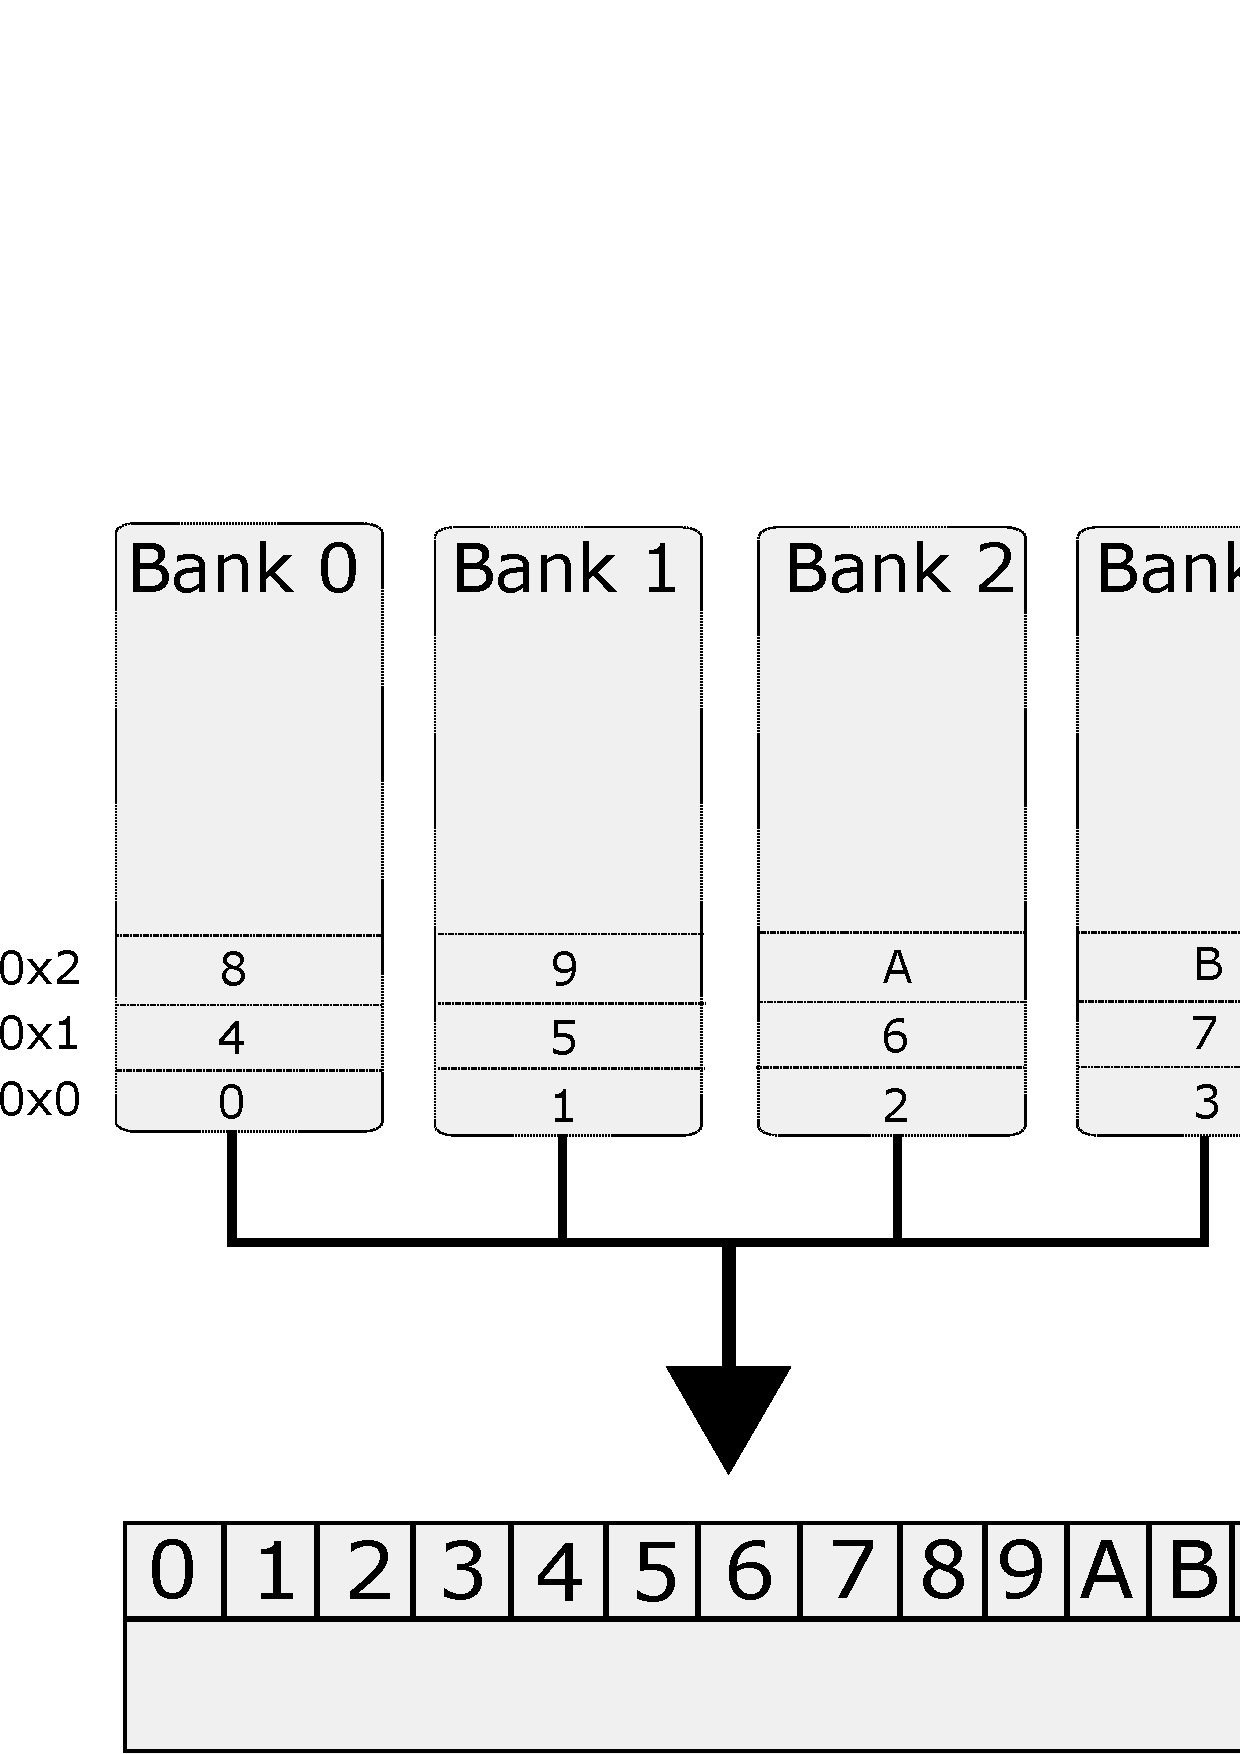
\includegraphics[width=.7\textwidth]{imgs/drawings/scalePost_explanation1.pdf}
 \caption{All following examples are based on this VRAM/Screen layout.}
 \end{figure}


 Drawing two columns (under pixel 0 and 1) can be done with only one pass using a VGA mask set to 3 to write in banks 0 and 1.\\
 \par
 \begin{minipage}{\textwidth}
\lstinputlisting[language=C]{code/pass_0_1.c}
\end{minipage}
\par

 \begin{figure}[H]
 \centering
 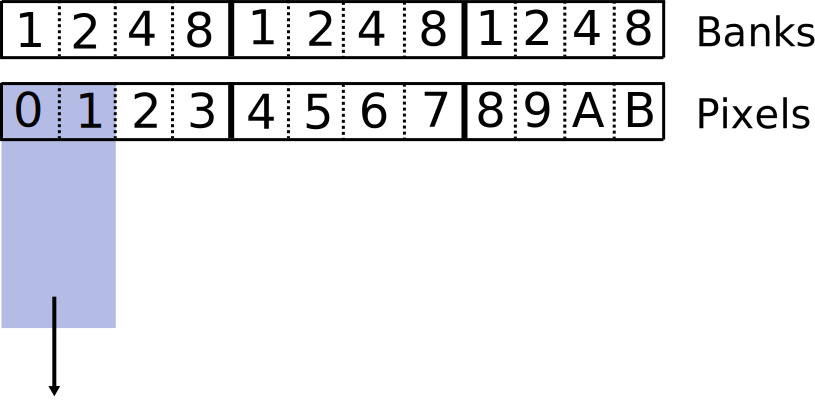
\includegraphics[width=.7\textwidth]{imgs/drawings/scalePost_explanation2.pdf}
 \end{figure}




\label{simd_vga}
If the two columns are not properly aligned (like columns under pixels 3 and 4), the mask is of no help. Two passes with mask set to 8 and then 1 will be needed.\\
 \par
 \begin{minipage}{\textwidth}
\lstinputlisting[language=C]{code/pass_3_4.c}
\end{minipage}
\par
  \begin{figure}[H]
 \centering
 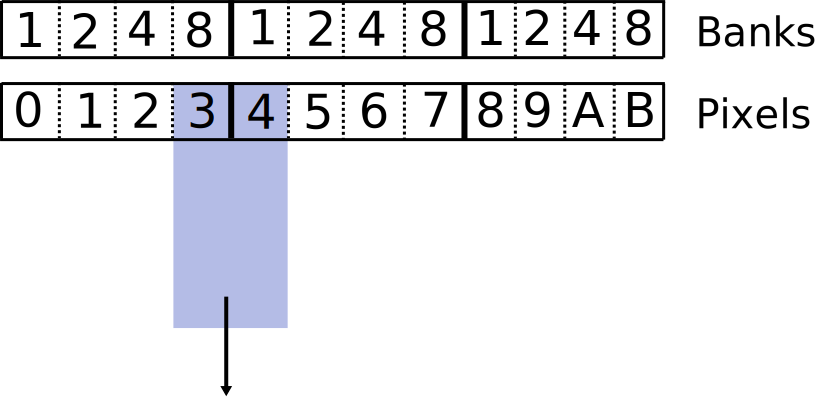
\includegraphics[width=.7\textwidth]{imgs/drawings/scalePost_explanation3.pdf}
 \end{figure}


In the worst case scenario, the engine needs to draw eight columns of pixels, under pixels 3,4,5,6,7,8,9 and A. Because of the poor alignment, three passes are needed with mask set to 8, 15 and, 7.\\
 \par
 \begin{minipage}{\textwidth}
\lstinputlisting[language=C]{code/pass_3_A.c}
\end{minipage}
\par
  \begin{figure}[H]
 \centering
 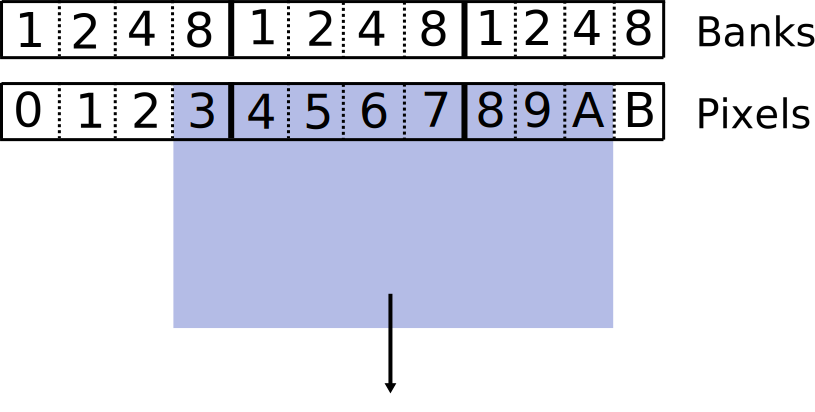
\includegraphics[width=.7\textwidth]{imgs/drawings/scalePost_explanation4.pdf}
 \end{figure}


% A better case where two passes with mask set to 15 then 3 allows drawing 6 columns of pixels :\\
%  \par
%  \begin{minipage}{\textwidth}
% \lstinputlisting[language=C]{code/pass_0_5.c}
% \end{minipage}
% \par
%    \begin{figure}[H]
%  \centering
%  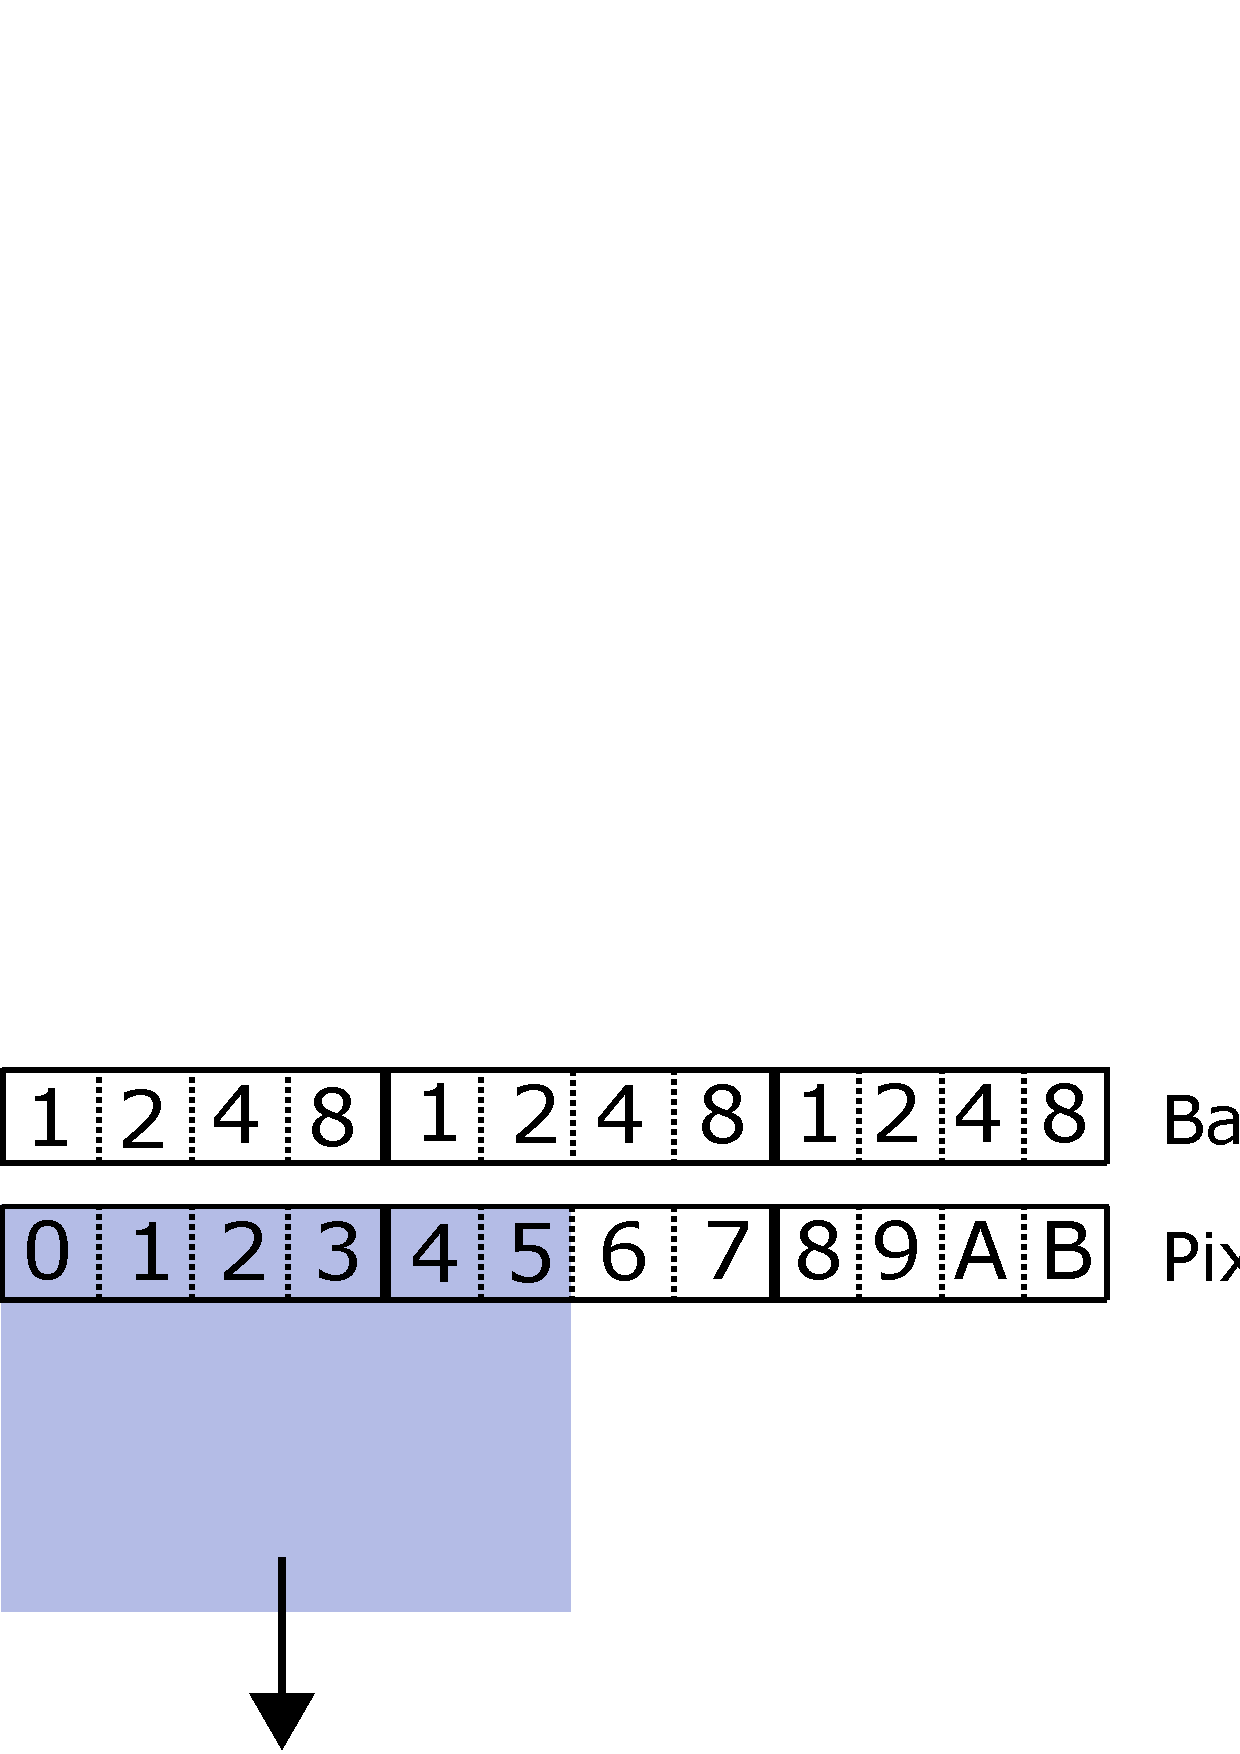
\includegraphics[width=.7\textwidth]{imgs/drawings/scalePost_explanation5.pdf}
  
%  \end{figure}






To visualize the performance gain in real cases, the engine has been modified to draw columns of pixels which were written "for free" thanks to the VGA mask manipulation in pink (page \pageref{wolf3d_in_pink} and \pageref{wolf3d_in_pink2}). We can see the performance improvement is significant, with 50\% of write operations avoided.

\trivia{Even though its was originally distributed exclusively as a shareware, sales called for a more "traditional" distribution. GT Interactive picked it up in 1993 and sold it in a nice box, along with the "Official Hint Manual". In 1995, the game was re-released on CD-ROM}.\\
\par
\fullimage{cover.png}


\begin{minipage}{\textwidth}
 \centering
 \scaledimage{0.9}{post_optimization_1_show.png} \label{wolf3d_in_pink}
\vspace*{0.5cm}\\
 \scaledimage{0.9}{post_optimization_1_pink_show.png}

\end{minipage}


\par

\begin{minipage}{\textwidth}
 \centering
 \scaledimage{0.9}{post_optimization_2_show.png} \label{wolf3d_in_pink2}
 \vspace*{0.5cm}\\
 \scaledimage{0.9}{post_optimization_2_pink_show.png}
\end{minipage}
This technique helps solve for scenarios where a large number of pixels have to be written due to the size of the wall. It only really shines when a lot of magnification occurs. For walls far away (minified) this technique doesn't help at all, but this matters less as small walls are cheap because they have fewer pixels
to render.\\
\par
\bu{Trivia :} Generating code at runtime may sound like an outdated technology. However, it was used as recently as 2016 when Android emulator used PixelFlinger to render the entire phone screen.





















\subsubsection{Texturing}
A subtle but extremely efficient trick used to improve the quality of the wall rendering is pre-baked light texturing. Wall texture assets were generated twice by the artists: once lit and once unlit.\\
\par
At runtime, upon finding ray-wall intersection, if the ray hits a vertical wall (looking at the map from above) on the Y axis, the engine uses a lit texture. If the ray hits an horizontal wall (on the X axis), it uses the unlit version of the same texture.\\
\par
 The difference is not obvious at first, but with the same scene rendered side by side with and without this effect, the visual difference is striking, giving the scene more realism because of this directional-light effect.\\
\par
  \begin{figure}[H]
\centering
 \fullimage{baked_lights_wood.png}
 \caption{Light and Dark wood textures.}
 \end{figure}
\par

\begin{minipage}{\textwidth}
\begin{figure}[H]
\centering
 \fullimage{backed_off.png}
 \caption{Above: Baked texture off. Below: Baked texture on.}
 \end{figure}

\begin{figure}[H]
\centering
 \fullimage{backed_on.png}
 
 \end{figure}
 \end{minipage}

 





\subsubsection{Doors}
Doors are rendered directly via the raycaster. Therefore, they have no thickness as that would have been much more complicated to implement.\\
\par
\begin{figure}[H]
 \centering
 \fullimage{door_flat.png}
\end{figure}

\par
Upon hitting a "DOOR" tile, the raycaster consults the \cw{doorposition} array. The raycaster is able to calculate how far along a door is opened and if it should either stop at the door or traverse through.\\

\begin{minipage}{\textwidth}
\lstinputlisting[language=C]{code/door.c}
\end{minipage}

\par 
 \par
\begin{figure}[H]
  \centering
 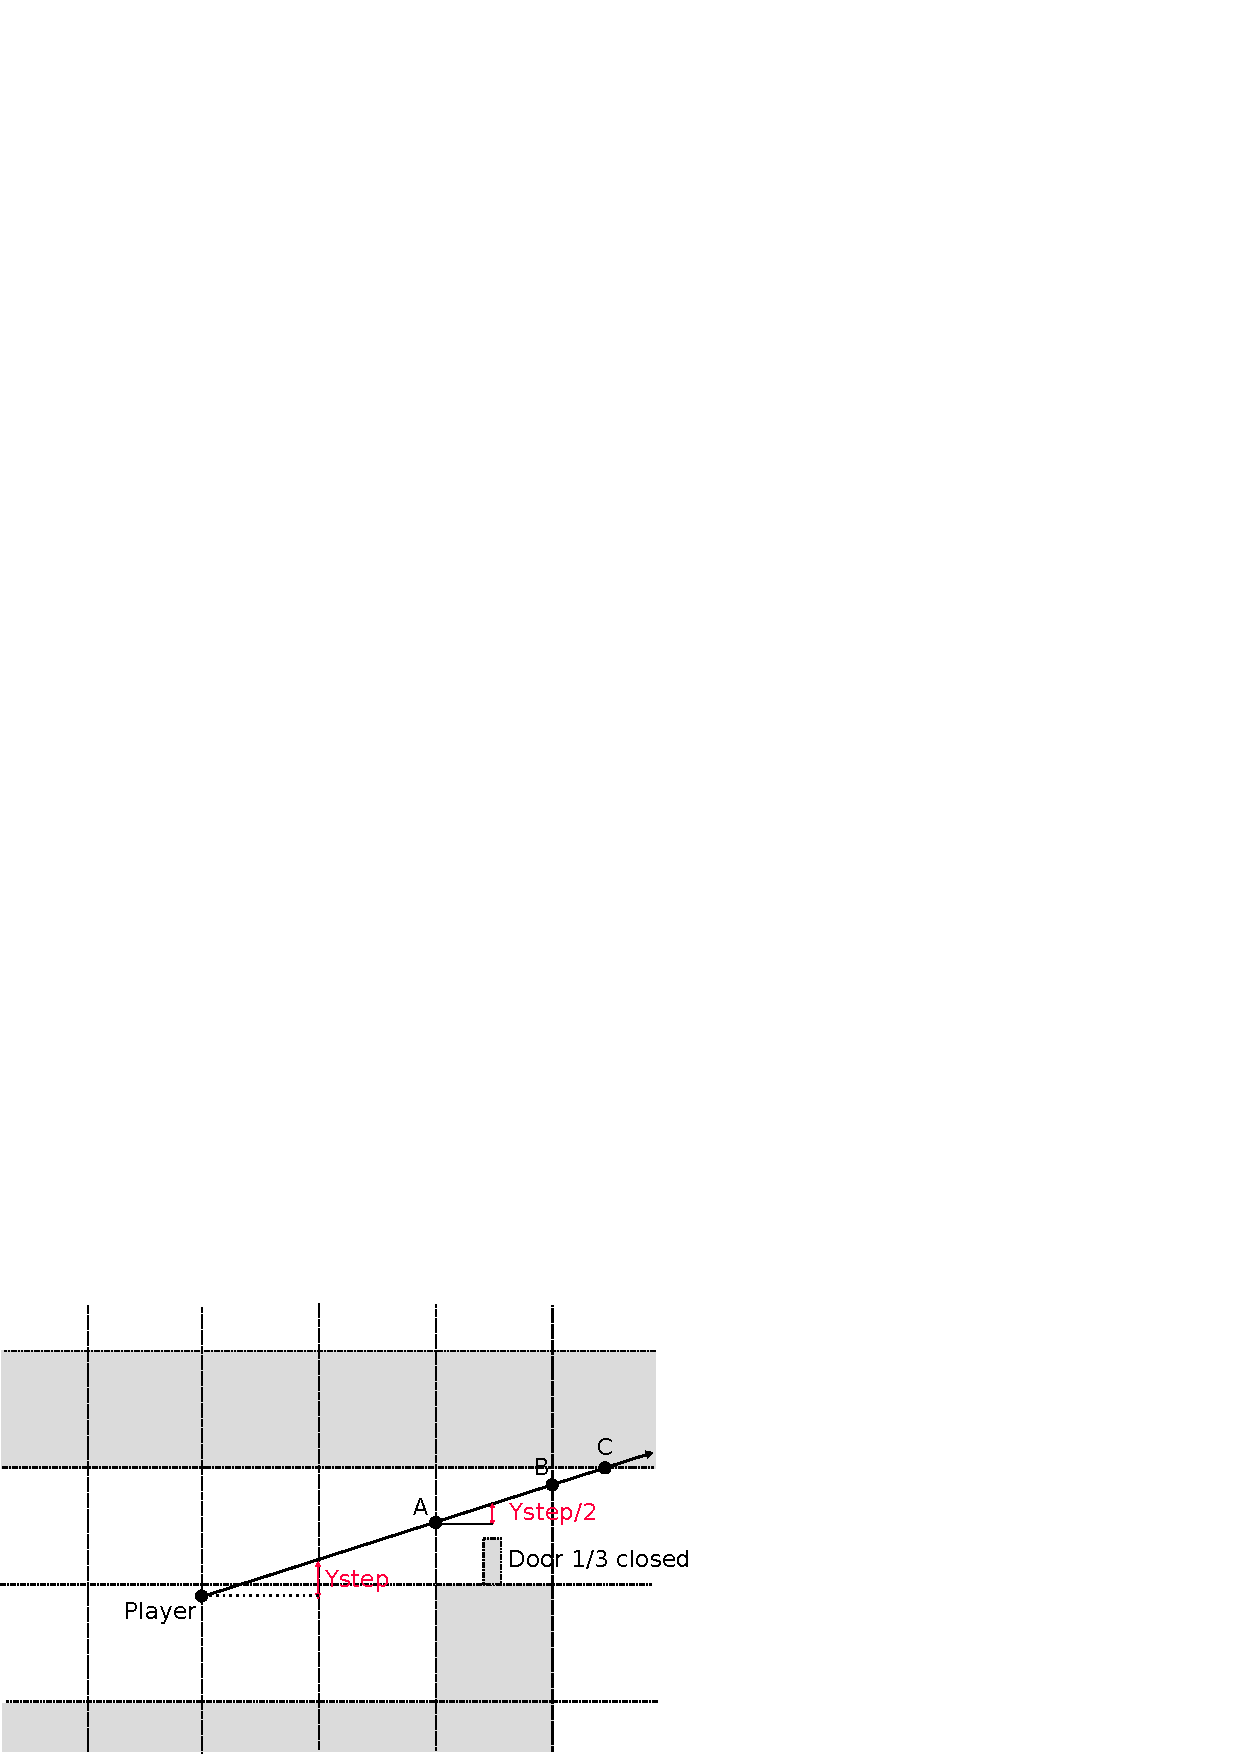
\includegraphics[width=\textwidth]{imgs/drawings/door_test.pdf}
 \caption{A ray traversing a partially opened door.}
\end{figure}
\par
Testing if a ray is stopped by a door or not costs almost nothing:\\
\par

\begin{equation*}
    \scalebox{1.3}{
$A_{X} + \dfrac{ystep}{2} < doorposition[doorIndex]$\\
}
\end{equation*}\\
\par
 In case of success, the ray traverses the wall tile and continues being tested against the grid. If the ray is a hit, the coordinates of the point of interception are calculated as $Intercept_{X} = A_{X} + \dfrac{ystep}{2}$ and $Intercept_{Y} = A_{Y} + \dfrac{TILE\_SIZE}{2}$ and passed to the renderer.












\subsubsection{Push Walls} 
Push walls are also implemented via the raycaster. Like doors, these moving walls are also treated as special cases. If the push wall has been activated, the raycaster adds an offset to the ray intercept coordinates.

















\subsection{Drawing Sprites}
\label{drawingSprites}
Once walls are drawn, it is time to render sprites such as enemies, items (ammo, weapons), and decorations (lamps, table, etc). This is a three step operation.
 \begin{enumerate}
  \item Identify which sprites are visible.
  \item Determine which part of the sprite is visible (not hidden by a wall).
  \item Draw what is visible.
 \end{enumerate}



\subsubsection{Visible Sprite Determination}
Building a list of visible sprites is done indirectly by leveraging information gathered by the raycaster. This relies on the assumption that visible sprites are on visible tiles. The raycaster marks all tiles visited by each ray while it travels the map looking for walls.\\
\begin{figure}[H]
  \centering
  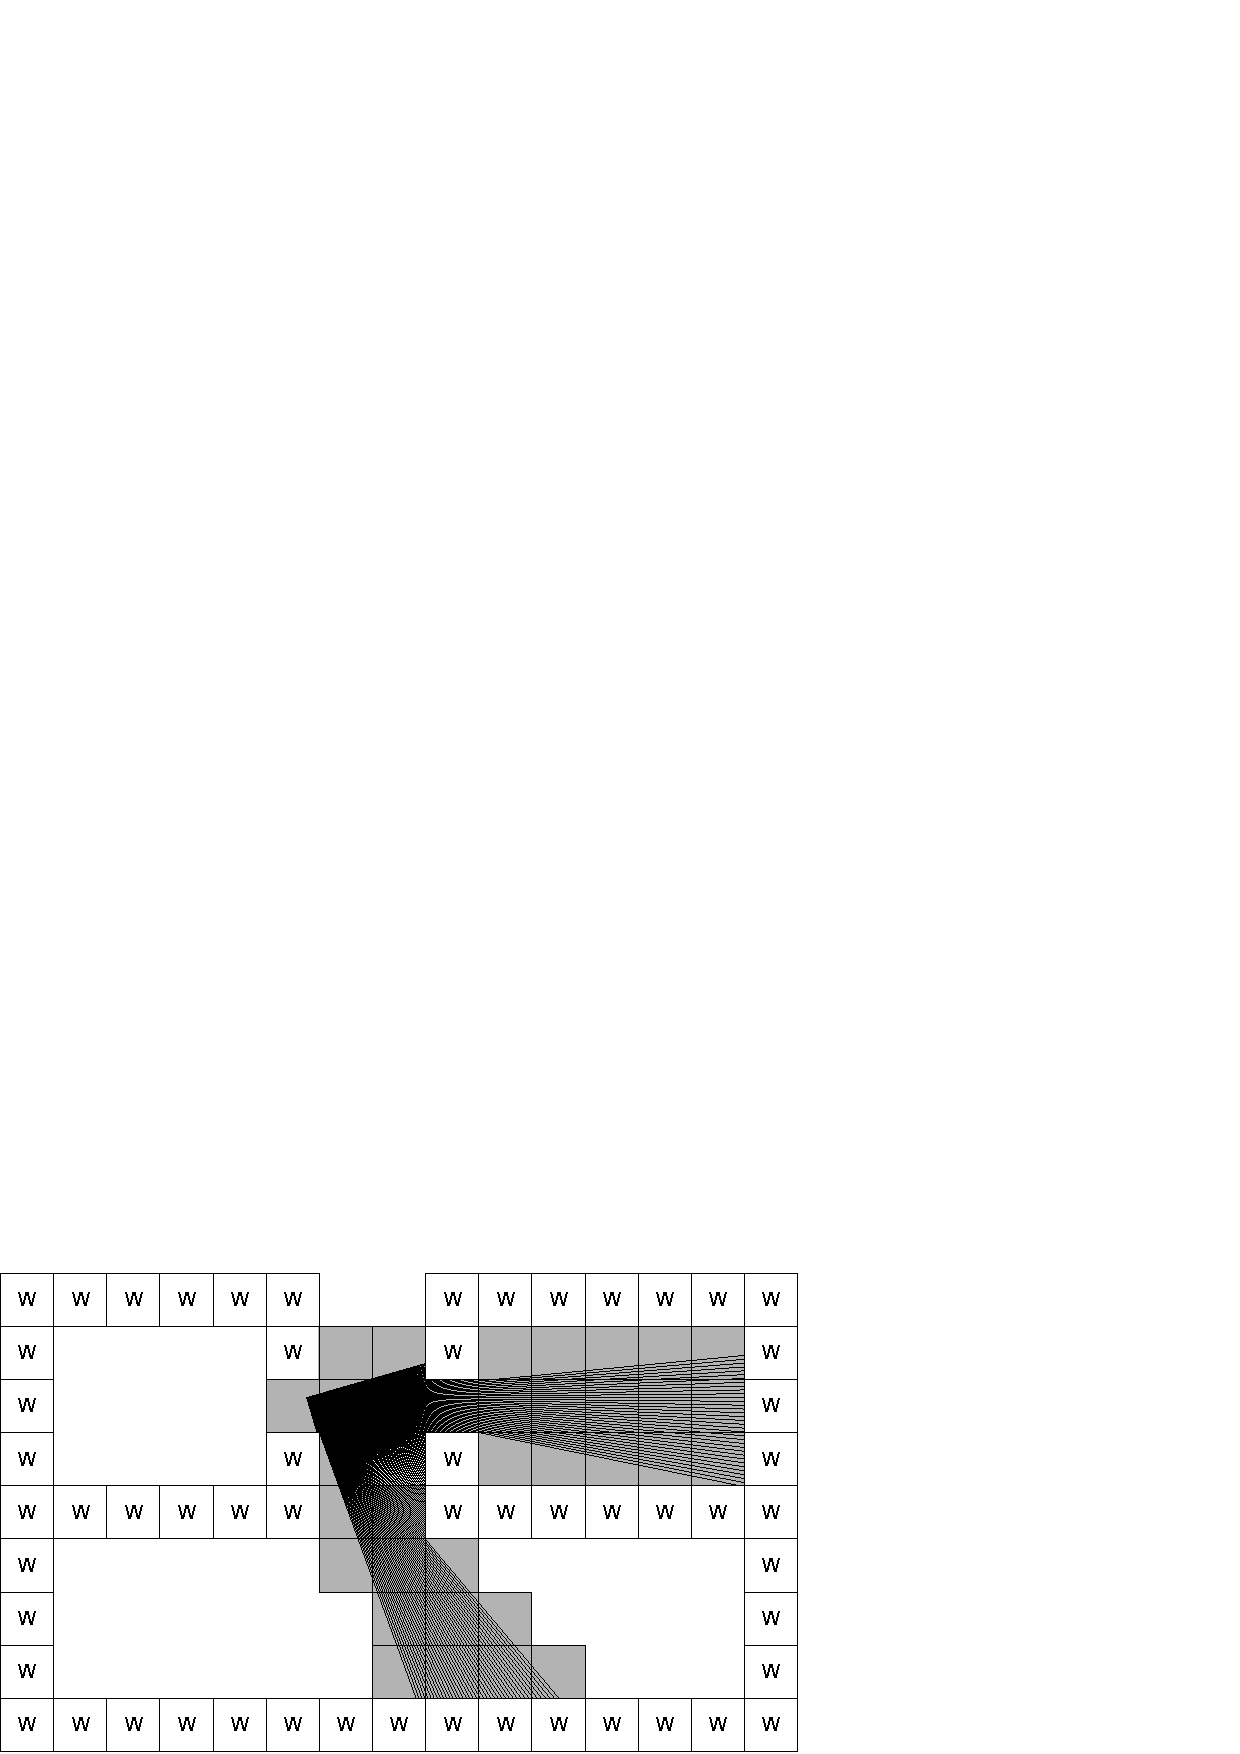
\includegraphics[width=\textwidth]{imgs/drawings/ray_caster_explained/marked_out_room.pdf}
 \caption{Ray casted and tiles marked as visible.} 
\end{figure}
Visible tile tracking is done in the simplest way with a 64x64 boolean array indicating if a tile was visited.\\
\par
\par
\begin{minipage}{\textwidth}
  \lstinputlisting[language=C]{code/spotvis.c}
\end{minipage}
\par

 At the beginning of each frame, the engine clears the array.\\
\par
\begin{minipage}{\textwidth}
 \lstinputlisting[language=C]{code/clear_vis_wold3d.c}
 \end{minipage}
 \par
The ray caster (\codeword{AsmRefresh}) writes \cw{true} in the \cw{spotvis} array as the ray progresses towards a wall. The array is used to select only visible objects:\\
\par
% \begin{minipage}{\textwidth}
%   \lstinputlisting[language={[x86masm]Assembler}]{code/mark_vis_wold3d.asm}
% \end{minipage}
% \par 

\par
\begin{minipage}{\textwidth}
 \lstinputlisting[language=C]{code/build_vis_list.c}
 \end{minipage}
 \par

While the way the visible tile array is used is not the most subtle part of the engine (it runs in $\mathcal{O}(n^2)$ time), it works well due to the low number of sprites. All sprites on the map are tested for visibility with \cw{spotvis}, then their height is calculated. They are all added to an array unsorted. A final double loop draws all sprites from far to near (using sprite height to determine distance on each iteration).\\ 




\subsubsection{Rendition}
Each sprite is rendered individually in the function \cw{ScaleShape (int xcenter, int shapenum, unsigned height)}. The sprite is transformed from map space to player space using the same SOH-CAH-TOA math seen in the "Drawing Walls" section.

\par
\begin{figure}[H]
\centering
 \includegraphics[width=\textwidth]{imgs/drawings/spaces.pdf}
 \end{figure}
\par
The X coordinate is used to place a sprite horizontally on the screen, while the Y coordinate is used for clipping. Like walls, sprites don't need to be placed vertically since they are drawn in the same 64x64 texels space.\\
\par
  \begin{minipage}{.5\textwidth}
     \fullimage{guard_sprite.png}
  \end{minipage}
   \begin{minipage}{.5\textwidth} 
     \fullimage{wall_texturw.png} 
   \end{minipage}

\par



 As shown in the following screenshot, scaling a vertically centered sprite is enough to give the illusion of perspective.\\
\par
\begin{figure}[H]
 \centering
 \fullimage{drawing_things.png}
\end{figure}

Sprites are special, however. Walls fill the full 64x64 space and are fully opaque, while sprites have transparent parts. For example, the "food" sprite is only 9 texels tall. The lamp sprite uses the full height but the middle is transparent.\\


  \begin{minipage}{.5\textwidth} 
     \fullimage{sprite_food.png} 
   \end{minipage}
  \begin{minipage}{.5\textwidth} 
     \fullimage{light_sprite.png}
   \end{minipage}

\par
\vspace{4mm}
\bu{Trivia :} Sprites with a lot of transparency (such as the two shown previously) would later turn out to be a major fillrate issue with the hardware accelerated renderer for the iOS port.\\
\par
\begin{fancyquotes}
Wolfenstein (and Doom) originally drew the characters as sparse stretched columns of solid pixels (vertical instead of horizontal for efficiency in interleaved planar mode-X VGA), but OpenGL versions need to generate a square texture with transparent pixels.  Typically this is then drawn by either alpha blending or alpha testing a big quad that is mostly empty space.  You could play through several early levels of Wolf without this being a problem, but in later levels there are often large fields of dozens of items that stack up to enough overdraw to max out the GPU and drop the framerate to 20 fps.  The solution is to bound the solid pixels in the texture and only draw that restricted area, which solves the problem with most items, but Wolf has a few different heavily used ceiling lamp textures that have a small lamp at the top and a thin but full width shadow at the bottom.  A single bounds doesn't exclude many texels, so I wound up including two bounds, which made them render many times faster. 
\bigskip \\
\textbf{John Carmack - Programmer}
 \end{fancyquotes}

\par












\subsubsection{Clipping}
Like everything in the game, sprites are made of and drawn as columns. Before drawing each column in a sprite, the engine determines for each column if it is occluded by a wall. This is called clipping and is an easy step thanks to walls and sprites being in the same 64x64 coordinate system. Once the sprite's position is transformed in player space, height is generated based on the distance Y. That height is the same as calculated for the walls. Therefore to determine if a sprite column is behind a wall, the engine simply compares its height to the height of the wall.\\
\par
In order to do that, the raycaster keeps tracks of each height calculated for each column in an occlusion array called \cw{wallheight}.\\
\par
\begin{minipage}{\textwidth}
\lstinputlisting[language=C]{code/wallheight_declaration.c}
\end{minipage}
\par
The occlusion array is written to during raycasting.\\
\par
\begin{minipage}{\textwidth}
\lstinputlisting[language=C]{code/wallheight_population.c}
\end{minipage}
While drawing sprites, the occlusion array is read. If the height of a wall is greater than that of a sprite, it means the wall is in front of the sprite and the full sprite rendition is skipped.\\
\par
\begin{minipage}{\textwidth}
\lstinputlisting[language=C]{code/wallheight_usage.c}
\end{minipage}
\par
Since the entire screen is refreshed on the next frame, the occlusion array does not need to be cleared at the beginning of a frame.\\


\begin{fancyquotes}
There was still a little more room for improvement in compiled scaler performance for wall textures:  if the textures were reorganized so that they went "middle-out", you could avoid half the loads by doing a 16 bit read and writing out AL for the top pixels and AH for the bottom pixels.\\
\par 
The combination of the compiled scalers getting more efficient at higher magnifications and the VGA latch writes avoiding entire columns let Wolf maintain almost the same speed with big walls and small walls, which was important.\\
\par
\textbf{John Carmack - Programmer}
 \end{fancyquotes}


\subsubsection{Drawing Things}
Sprite rendering benefits from the same optimization we saw in walls (compiled scalers and deferred rendering). However, since sprites introduce transparency the techniques are slightly adjusted.

\subsubsection{Compiled Scalers}
Visible sprite column rendition is also done with the compiled scalers, but the scalers cannot be used directly. A compiled scaler draws its speed from its absence of parameters. It is an unrolled loop hardcoded with x86 instructions to read from a texture 64 texels tall and write/scale a predetermined number of pixels. For example, compiled scaler \#112 always reads 64 pixels of texture and magnifies it to 134 pixels on the screen. Transparency is not handled at all, used as is the scalers would draw transparent pixels in pink. To solve this problem, sprites are stored in a special way that allows tweaked compiled scalers to skip transparency.\\
\par
A sprite is stored as an array of 64 entries. Each entry is a series of "commands" forming a column. A command features:
\begin{enumerate}
 \item A vertical offset.
 \item A vertical length.
 \item A payload of texels.
 \end{enumerate}
\par
The last command in a column is marked with an offset of \cw{0x00}.\\
\par

\begin{minipage}{.5\textwidth}
\bu{Example :} Column \#25 in the lamp sprite is made of 5 transparent pixels, followed by one sequence of 5 pixels for the lamp:\\
\par
\scaledimage{0.8}{light_sprite_column_head.png}
\par
Followed by 49 transparent pixels, and finally one sequence of 5 pixels for the light halo.\\
\par
\scaledimage{0.8}{light_sprite_column_bottom.png}
\par
Total: 64 texels. This column is encoded with 2 commands of 1 byte offset +  1 byte length + 5 bytes of payload. A payloadless command with length 0x00 marks the end. Total size is 17 bytes.\\
 \end{minipage}
\begin{minipage}{.5\textwidth}
\begin{figure}[H]
  \begin{flushright}
     \scaledimage{0.9}{light_sprite_column.png}
   \end{flushright}
\end{figure}
\end{minipage}



 
\par
The idea is to prevent a scaler from consuming 64 texels by patching the x86 instructions with an early return instruction \cw{ret}. In order to do that, the code generator also generates patch locations. The \cw{t\_compscale} structure containing a compiled scaler not only features the x86 instruction in \cw{code}, it also features patching offset.\\
\par
\begin{minipage}{\textwidth}
\lstinputlisting[language=C]{code/t_compscale.c}
\end{minipage}
\par
There are 64 patch locations per scaler (one for each length of pixels from 0 to 63, stored in \cw{codeofs[]}), which allows for writing a \cw{RETF} instruction causing an early return. For each command in a sprite column, the engine looks up how many texels the command payload contains and where to patch the scaler, then saves the instruction at this location and overwrites it with a \cw{RETF}. After the scaler returns (and the command payload has been rendered), the scaler is unpatched.\\
\par
In the assembly optimized code, note how the engine knows where to patch the code thanks to a \cw{BX} register which points to \cw{codeofs}.\\
\par
\begin{minipage}{\textwidth}
  \lstinputlisting[language={[x86masm]Assembler}]{code/self_modifying.asm}
\end{minipage}
\par
Patching the scaler is not enough. It only allows for consuming less than 64 texels. In order to draw a "hole" properly on screen, the engine also needs to know how many pixels to skip vertically in screenspace before starting the scaler on the next command. This is where the \cw{width[]} array is used. The scaler generator also saves 64 entries to convert sprites' transparent height into screen space height.\\


\subsubsection{Deferred Rendering}
The same deferred drawing technique we saw for walls is also used for sprites, and is especially powerful when a sprite is magnified.\\

\par
\begin{figure}[H]
 \centering
 \fullimage{magnified_enemy_before.png}
\end{figure}
In this scene, the 64x64 guard sprite is magnified 2.2 times. By zooming in, we see that each column is repeated at least twice and sometimes three times. It is a perfect optimization case for VGA mask manipulation.\\
\par
A modified version of the engine (which draws "free" columns in pink) is again used to demonstrate.  In this case most columns were drawn only once. Magnification was a totally free operation despite more than twice the number of texels written to the screen.\\

\par
\begin{figure}[H]
 \centering
 \fullimage{magnified_zoom.png}
\end{figure}
\begin{figure}[H]
 \centering
 \fullimage{maginfized_zoom_modified.png}
\end{figure}






\subsection{Drawing Weapons}
Drawing the weapon at the bottom of the canvas is straight forward. It uses the same type of rendering as sprites but with clipping disabled (in the function \cw{ScaleShape}). The same compiled scaler and deferred rendering tricks are used.














\subsection{A.I}
To simulate enemies, some objects are allowed to "think" and take actions like firing, walking, or emitting sounds. Those thinking objects are called "actors".\\
\par






Actors are programmed via a state machine. They can be aggressive, sneaky, or dumb (rockets for instance). To model their behavior, all enemies have an associated state:
\begin{itemize}
\item Standing
\item Attack
\item Path
\item Pain
\item Shoot
\item Chase
\item Die
\item Special Boss
\end{itemize}

Each state has associated \cw{think} and \cw{action} method pointers. There is also a \cw{next} pointer to indicate which state the actor should transition to when the current state is completed.\\
\par
\begin{minipage}{\textwidth}
\lstinputlisting[language=C]{code/statetype.c}
\end{minipage}
\par


A guard in standing position always stays in the same state (\cw{next} points to itself):\\
\par

\begin{minipage}{\textwidth}
\lstinputlisting[language=C,style=mystyle,basicstyle=\small,morekeywords={statetype, NULL, true, false}]{code/s_grdstand.c}
\end{minipage}
\par
Some state chains are more complex, as with chasing:\\

\par
\begin{minipage}{\textwidth}
\lstinputlisting[language=C,style=mystyle,basicstyle=\small]{code/s_grdchase.c}
\end{minipage}
\par

\begin{fancyquotes}
The enemies in Wolf felt different based on the decision to close distance to the player either largest or smallest axis delta first - Closing smallest first made the brown shirts line up with you a long way away, making them easy to shoot.  Closing largest first made the officers come at you in a ragged diagonal, as if they were dodging your shots.\\
\par
\textbf{John Carmack - Programmer}
 \end{fancyquotes}
\par
All types of enemies (including bosses) have their own state machine. They often share actions (e.g. \cw{T\_Stand} and \cw{T\_Path}) but also occasionally have their own.\\
\par
What makes enemies interesting is how they trigger from standing to aggressive via \cw{T\_Stand}. They have three ways to detect the player:
\begin{itemize}
\item Proximity
\item Sight
\item Noise
\end{itemize}
By far the most important stimuli and, what makes the player feel like the A.I is "smart", is reaction to noise.





\subsubsection{Sound Propagation}
Early on the game teaches the player that enemies react to gunfire and seek out the source. Sound is an essential part of the experience and propagating it realistically in realtime is hard.\\
\par
 A floodfill algorithm could have been used but that would have been slow. To speed things up, maps are preprocessed. Each room delimits an area. At runtime the engine maintains a matrix of portals connecting areas and updates it when a door opens or closes. Determining if an enemy can hear the player's gunfire is then a simple lookup in a table.

\par
\begin{figure}[H]
 \centering
 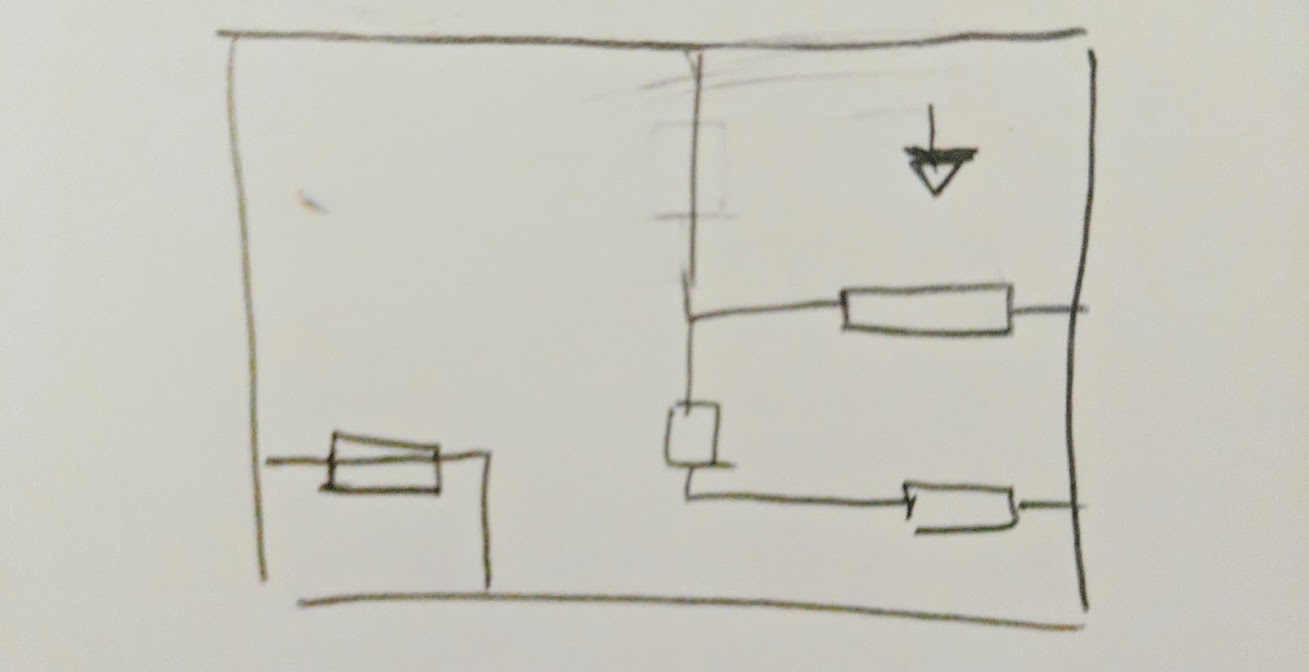
\includegraphics[width=.73\textwidth]{imgs/drawings/sound_area/map.pdf}
 
\end{figure}

\par
\begin{figure}[H]
 \centering
 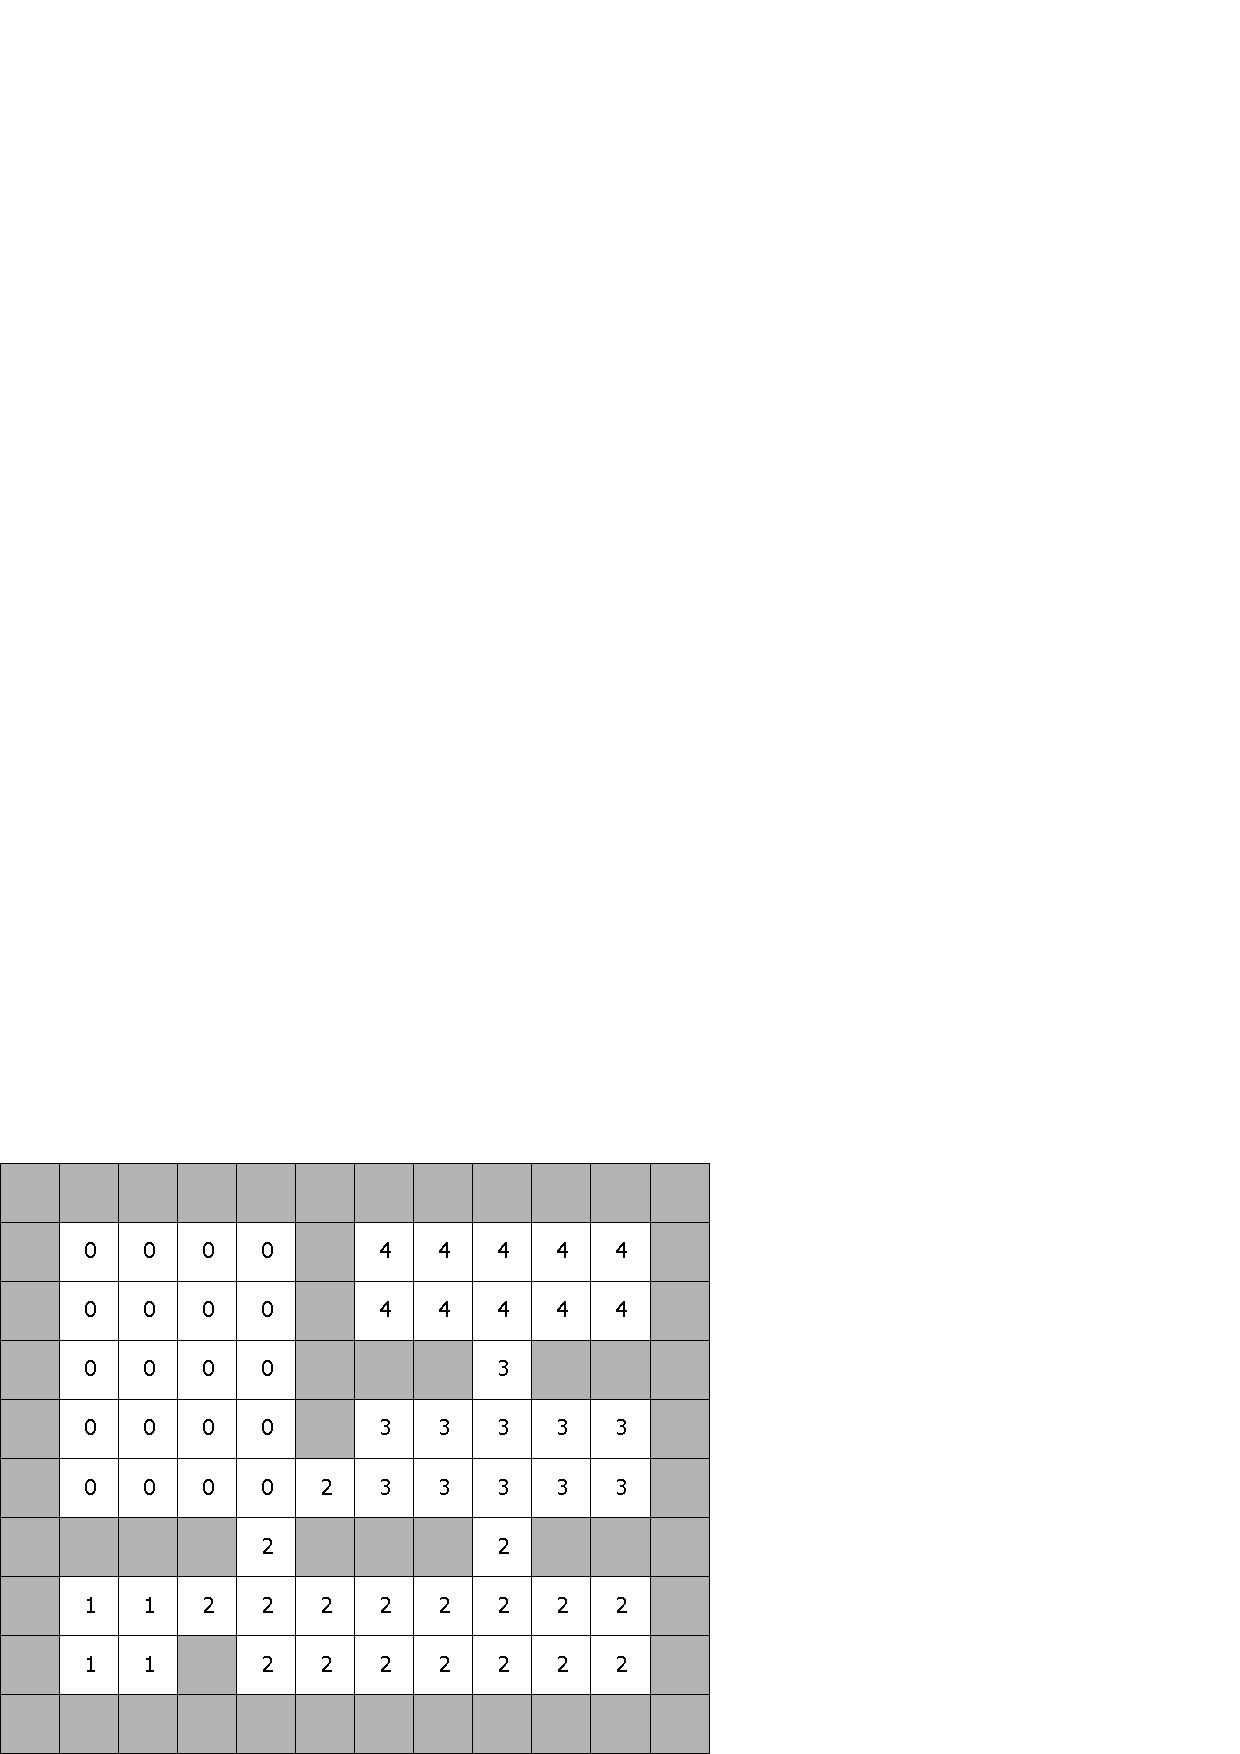
\includegraphics[width=.73\textwidth]{imgs/drawings/sound_area/area.pdf}
 \caption{A map generated by TED5 before and after preprocessing for audio propagation. After processing each block must belong to an area.}
\end{figure}
\par



\begin{figure}[H]
 \centering
 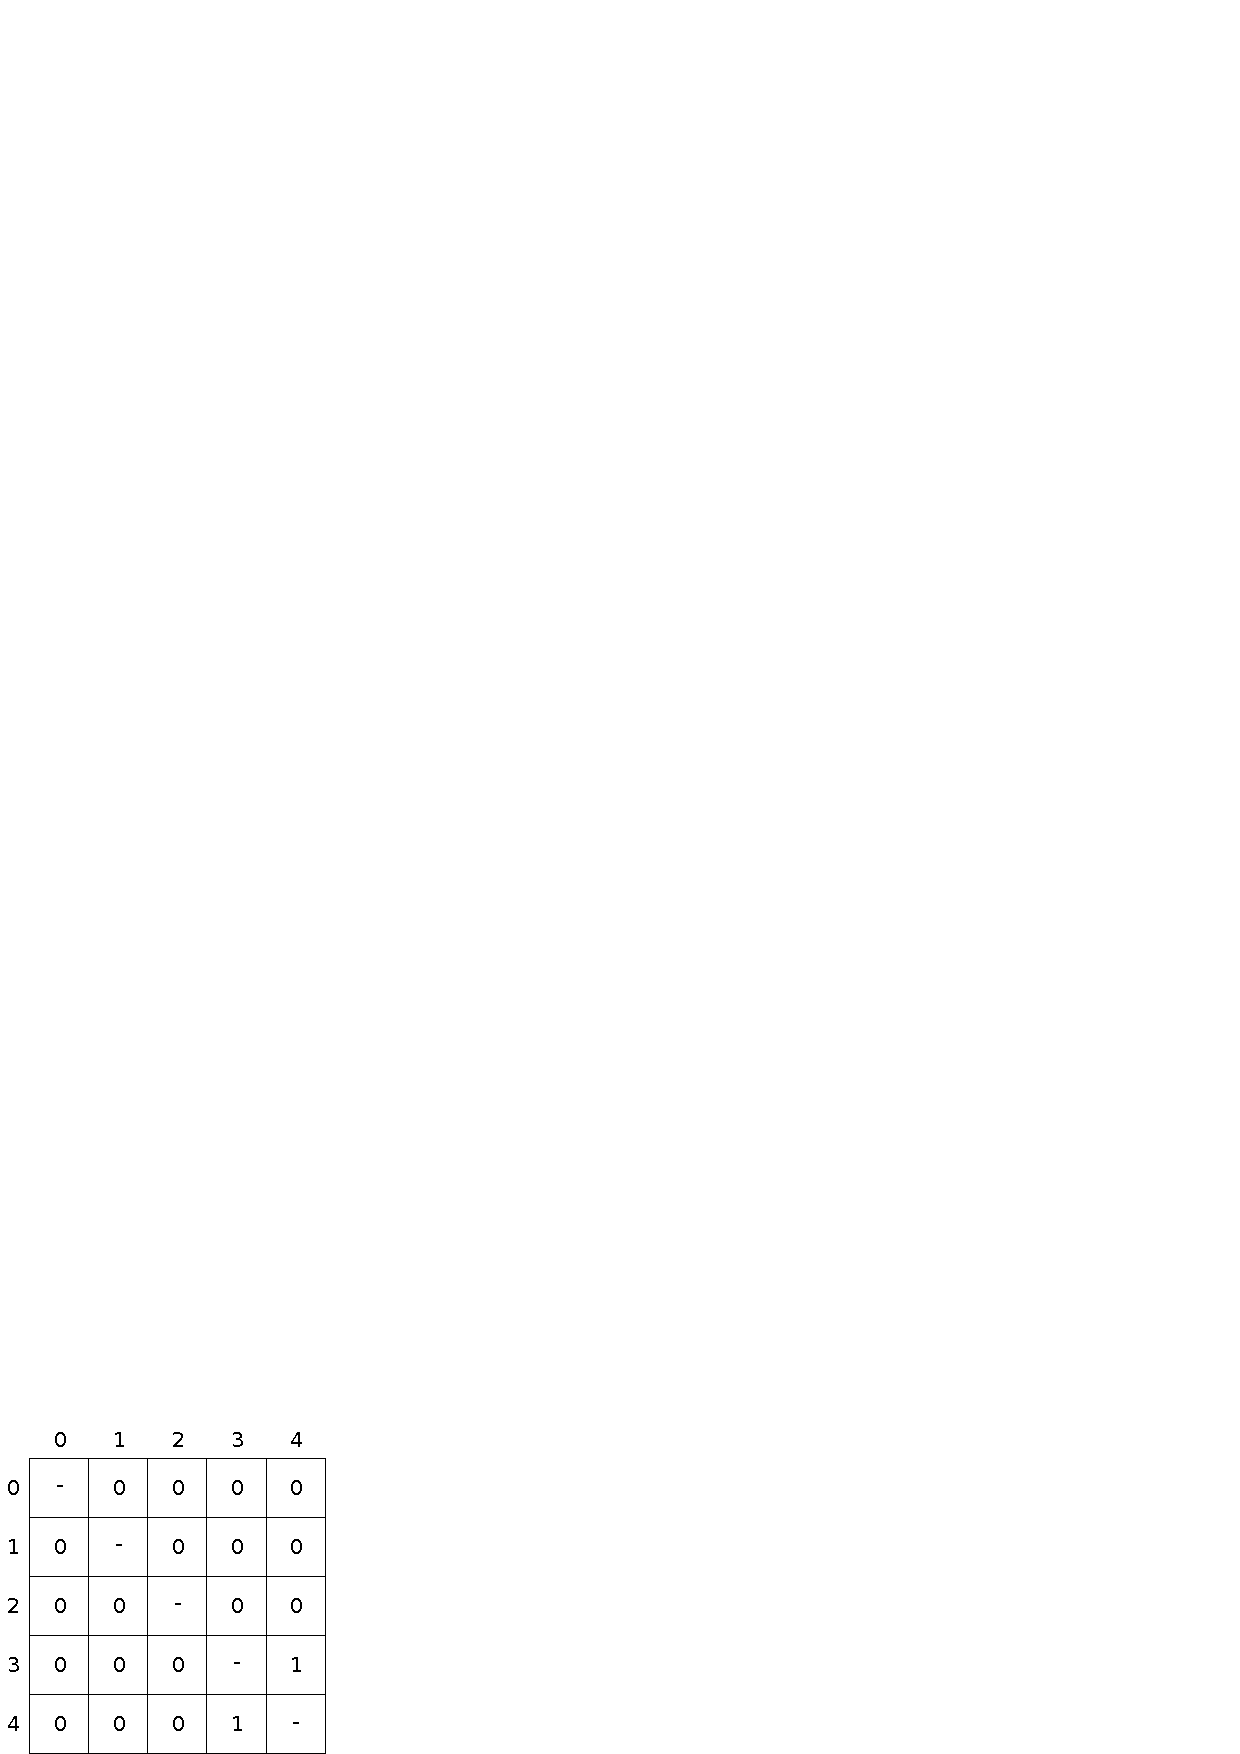
\includegraphics[width=.5\textwidth]{imgs/drawings/soud_propagation/areaconnect.pdf}
\end{figure}
\par
At runtime the engine maintains a matrix of portals. Each time a door is opened or closed, the array \cw{areaconnect[][]} is updated and \cw{areabyplayer[]} array is populated recursively starting with \cw{areabyplayer[player.tile] = 1}. If player is in area 4 and open the door to 3, \cw{areabyplayer[]} will look as follow.
\par
\begin{figure}[H]
 \centering
 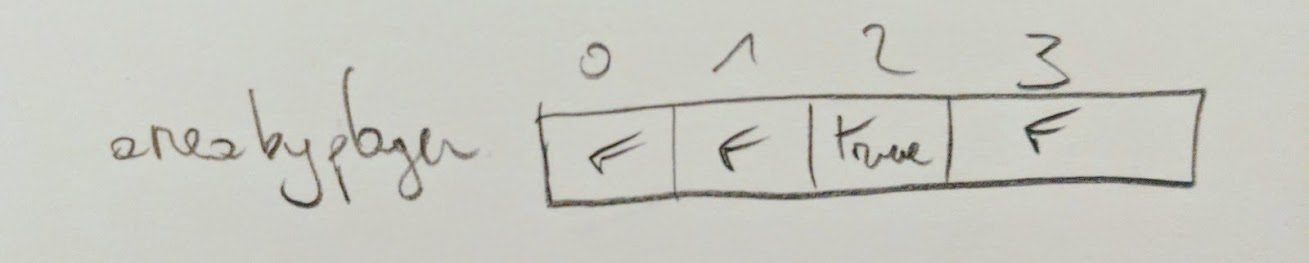
\includegraphics[width=.5\textwidth]{imgs/drawings/soud_propagation/areabyplayer.pdf}
\end{figure}
\par
Determining if an enemy in area X can hear the player is achieved with an inexpensive lookup in \cw{areabyplayer[X]}.\\
\par
\begin{minipage}{\textwidth}
\lstinputlisting[language=C]{code/num_areas.c}
\end{minipage}
\par
%\cw{NUMAREAS = 37} seems like a random value. It was likely obtained empirically with the developers bumping it up every time they designed a map which crashed the engine.\\
\par







\subsubsection{Sound Non-propagation}
Perfect sound propagation is a simplistic model. When a gun is fired, all enemies which can hear it will shout "Achtung!" (Attention!) and converge toward the origin of the sound. This would get old pretty fast, though. To make gameplay spicier, the designers introduced a little hack that goes a long way in making the AI appear smarter than it is.


\par
\begin{minipage}{1\textwidth}
\begin{figure}[H]
 \centering
 \fullimage{ambush/map_unknown.png}
\end{figure}
\par


  \begin{minipage}{0.6\textwidth}
  There is a perfect example early on in the game in map E1M1.\\
  \par At this point, the player has learned that enemies will react to gunfire and move toward its origin. Upon entering this room and dispatching the guard, she naturally assumes this is a safe place -- a bounded area where no other enemies can be encountered (otherwise they would have shown up or at least shouted by now).
  \end{minipage}
  \begin{minipage}{0.4\textwidth}
  \begin{flushright}
  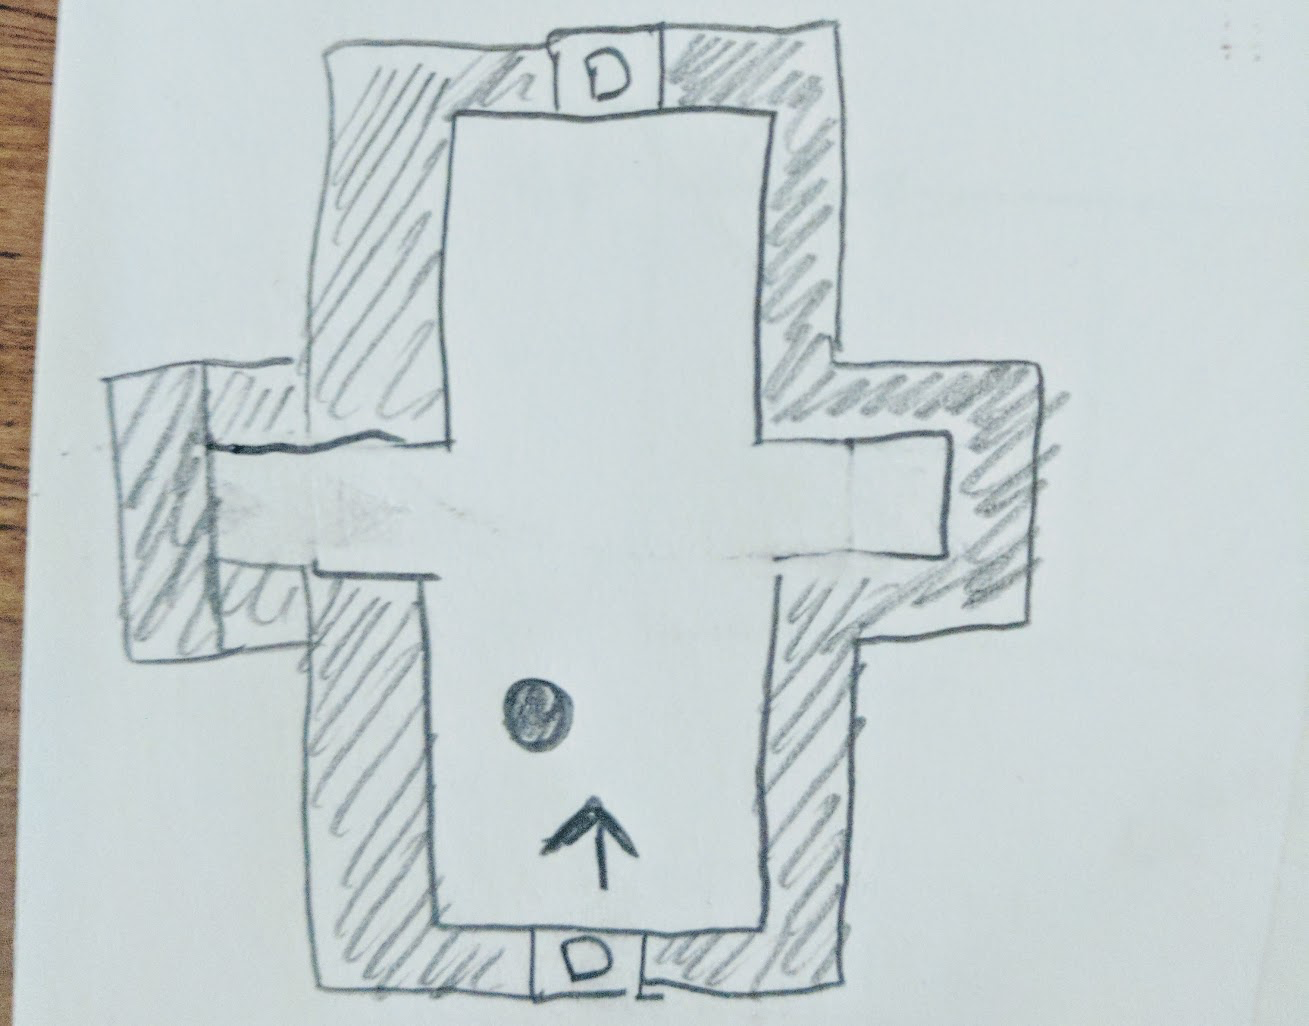
\includegraphics[width=0.9\textwidth]{imgs/drawings/ambush/map_unknown_drawing.pdf}
  \end{flushright}  
  \end{minipage}
\end{minipage}
\noindent
\\


\par
\begin{minipage}{1\textwidth}
  \begin{figure}[H]
   \centering
   \fullimage{ambush/map_ambushed.png}
  \end{figure}
  \par
  \begin{minipage}{0.6\textwidth}
  Feeling safe, she will either run straight to the door or go left (or worse: right) to see what is in these corners. Surprise! An enemy was "hiding". This behavior is possible thanks to special tiles marked "AMBUSH" which make the engine not propagate sound to actors standing on these tiles.\\
  \par
   This is probably one of the cheapest features in the engine, yet it results in what most would agree is the soul of the game - keeping the player on her toes.
  \end{minipage}
  \begin{minipage}{0.4\textwidth}
  \begin{flushright}
  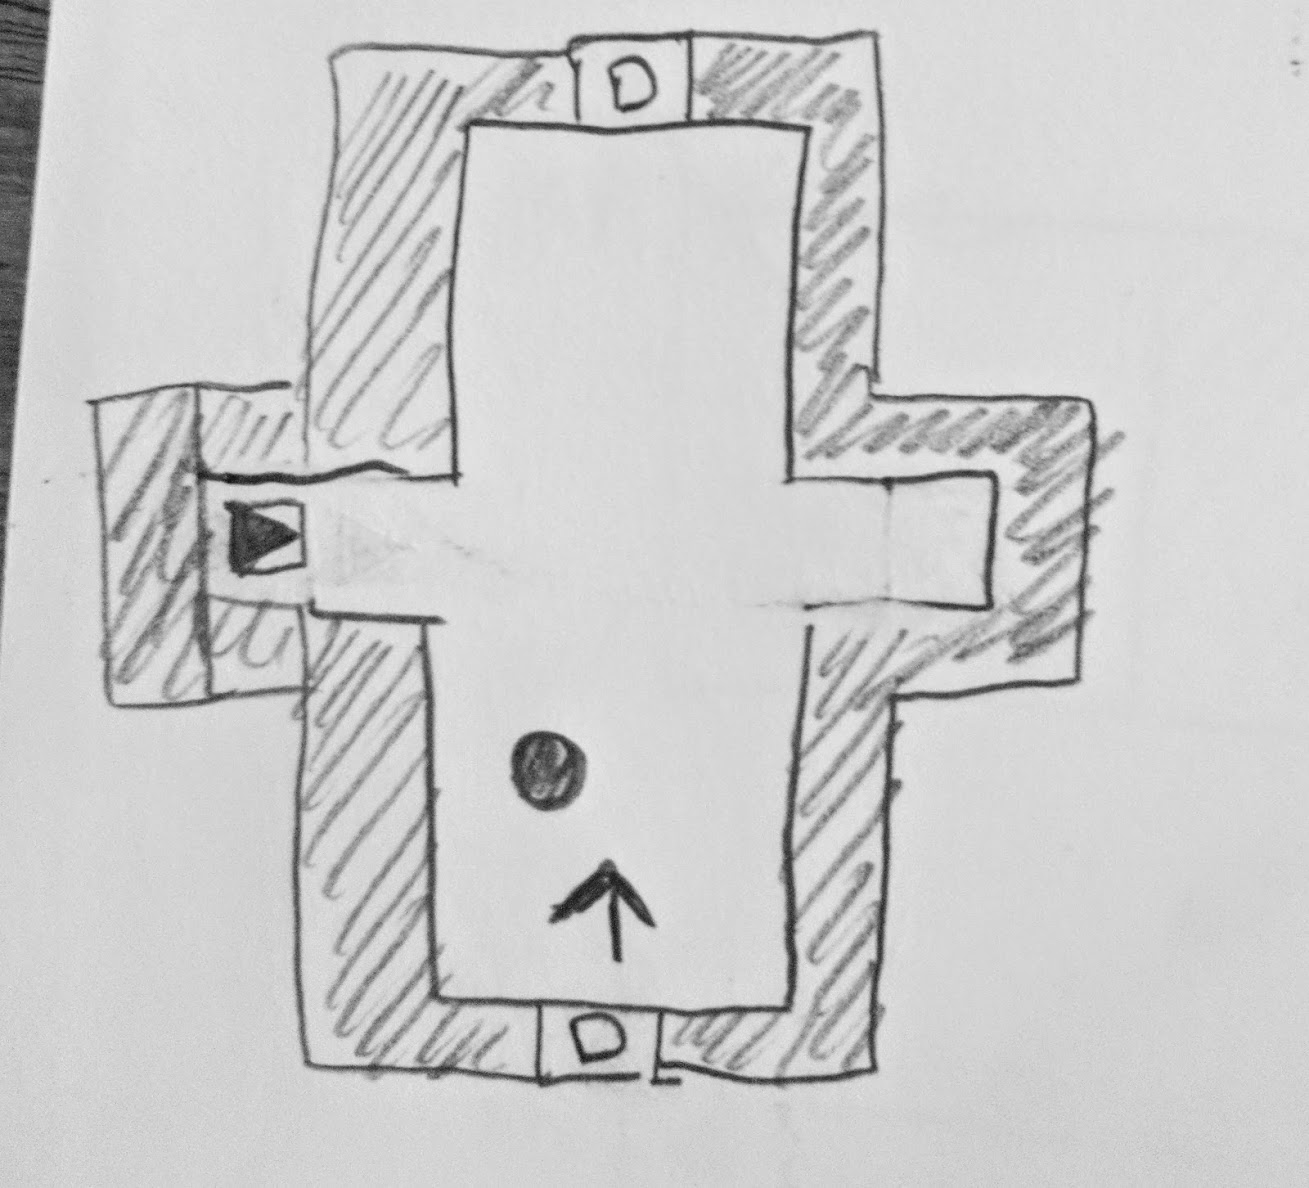
\includegraphics[width=0.9\textwidth]{imgs/drawings/ambush/map_ambushed_drawing.pdf}
  \end{flushright}
  \end{minipage}
\end{minipage}


\par

\bu{Trivia :} The ambush behavior is explained in the Hint Book as follows:\\
\par
\begin{fancyquotes}
Each enemy is given specific orders which dictate his actions once he knows of your presence. Some are ordered to immediately attack, while others are trained to act only upon visual contact.\\
\par
\textbf{Kevin Cloud. The Official Hint Manual for Wolfenstein 3D}
 \end{fancyquotes}
\par
\bu{Trivia :} Be it bug or dedication, a guard on an \cw{AMBUSH} tile will react ONLY to seeing the player. Seeing another actor/dog die right in front of him will not activate him.\\


\subsubsection{Patrolling}
In "path" mode, an agent simulates patrolling. There is no path finding; this is all done via waypoints which change the direction of the agent. After stepping on a "change direction" tile, the agent keeps on walking straight until it hits a wall. All waypoints are manually placed by the map designer with TED5.\\ 
\par
The waypoint system was used in other creative ways, like in E1M1 to simulate the agitation of German shepherds (marked a "D"). A detailed view of the right wings of the map from page \pageref{mape1m1} shows no less than eight waypoints making the dogs run in circles and zigzag.\\
\par
\begin{figure}[H]
 \centering
 \scaledimage{0.8}{path.png}
\end{figure}
\par




